
\documentclass[bibliography=totoc,listof=totoc,BCOR=5mm,DIV=12]{scrbook}
\usepackage[utf8]{inputenc}
\usepackage{graphicx}
\usepackage[hyphens]{url}
\usepackage{hyperref}
\usepackage[nohyperlinks,printonlyused,withpage]{acronym}
\usepackage{enumitem}
\usepackage{multirow}
\usepackage{tabularx}
\usepackage[table,dvipsnames]{xcolor}
\usepackage{amssymb}
\usepackage{ulem}
\usepackage{amsmath}
\usepackage{subcaption}
\usepackage{listings}
\usepackage{tikz}
\usepackage{pifont}
\usepackage{scrhack}
\usepackage{bookmark}
\newcommand{\xmark}{\textcolor{Mahogany}{\ding{55}}}%
\newcommand{\cmark}{\textcolor{OliveGreen}{\ding{52}}}%
\usetikzlibrary{matrix}
\graphicspath{{./Bilder/}}
%\renewcommand{\UrlFont}{\tiny\texttt}

\input{hyphenation}

\newcommand{\footurl}[1]{\footnote{{\url{#1}}}}
\newcommand{\bigo}{\mathcal{O}}
\begin{document}

% ---------------------------------------------------------------
\frontmatter
    %%%%%%%%%%%%%%%%%%%%%%%%%%%%%%%
% erste Seite

\thispagestyle{empty}

\begin{center}

\vspace*{-2cm}

{\Huge INSTITUT FÜR INFORMATIK\\[1mm]}
DER LUDWIG--MAXIMILIANS--UNIVERSITÄT MÜNCHEN\\

\vspace*{1cm}

\includegraphics[width=0.3\textwidth]{lmu_siegel}

\vspace*{2cm}

{\Large \textbf{Masterarbeit}}\\ % oder Fortgeschrittenenpraktikum, Master's Thesis, Bachelorarbeit etc.

\vspace{2.0cm}
{\Huge \textbf{Towards Quantum-Resistant MACSec using EAP-TLS}}\\

{\LARGE Robin Lösch} % Name des Autors

\vspace{3cm}
%Draft vom \today % erleichtert den Betreuern die Zuordnung - für finale Version entfernen

\end{center}

\newpage

%%%%%%%%%%%%%%%%%%%%%%%%%%%%%%%
% zweite Seite

\thispagestyle{empty}
\cleardoublepage

%%%%%%%%%%%%%%%%%%%%%%%%%%%%%%%
% dritte Seite (Kopie der ersten)

\thispagestyle{empty}

\begin{center}

\vspace*{-2cm}

{\Huge INSTITUT FÜR INFORMATIK\\[1mm]}
DER LUDWIG--MAXIMILIANS--UNIVERSITÄT MÜNCHEN\\

\vspace*{1cm}

\includegraphics[width=0.3\textwidth]{lmu_siegel}

\vspace*{2cm}

{\Large \textbf{Masterarbeit}}\\ % oder Fortgeschrittenenpraktikum, SEP etc.

\vspace{2.0cm}
%{\Huge \textbf{Post-Quantum Key Exchange and Authentication for IEEE 802.1AE}}\\
%{\Huge \textbf{Towards Quantum-Resistant Cryptography for IEEE 802.1AE}}\\
{\Huge \textbf{Towards Quantum-Resistant MACSec using EAP-TLS}}\\

\vspace{1.5cm}

{\LARGE Robin Lösch} % Name des Autors
\vspace{2cm}

\parbox{1cm}{
\begin{large}
\begin{tabbing}
Aufgabensteller: \hspace{.5cm} \=Prof. Dr. Dieter Kranzlmüller\\[2mm]
Betreuer:
\>Sophia Grundner-Culemann\\
\>Dr. Tobias Guggemos\\
\>Dr. Joo Cho, ADVA Optical Networking\\[5mm]
Abgabetermin: \> 19. Januar 2021\\
\end{tabbing}
\end{large}}\\
\vspace{5mm}

\end{center}

    \thispagestyle{empty}
    \cleardoublepage
    \include{./Titel/erklaerung-lmu}
    \thispagestyle{empty}
    \cleardoublepage
    \vspace*{2cm}

\begin{center}
    \textbf{Abstract}
\end{center}

\vspace*{1cm}

\noindent In the last 40 years, quantum computing developed from an exclusively theoretical description of a quantum Turing machine to real-world implementations with various technologies and capabilities. Linking this development to digital computer's rapid development in the 20th century, a quantum computer with practical implications on industry and everyone's daily life seems within reachable bounds. There are many reasons to seek such a practical implementation. From algorithmic improvements to completely new technical possibilities like quantum teleportation, a quantum computer promises to solve certain tasks faster than possible with a classical digital computer.

\par Besides the benefits such a computer could provide, it would also have a significant impact on cryptography. Modern cryptography protocols in general and especially the field of public-key cryptography relies on mathematical problems that are believed to be intractable. Famous examples of such algorithms are the RSA and the Diffie-Hellman (DH) key exchange protocol and its variant, Elliptic Curve Diffie-Hellman (ECDH). Today, nearly all encrypted messages in the modern Web are bootstrapped by either one of these protocols. A serious flaw in these cryptosystems would have a massive impact on the confidentiality of user data. This is where quantum computing comes into play. In 1999 Peter Shor published his famous algorithm, which uses a quantum computer to break both the RSA and the DH problem. Since Shor was able to show that both algorithms run in polynomial time, the foundation of modern cryptography is questioned.

Luckily, even more than 20 years later, there is no implementation of a quantum computer available that could be used to break cryptographic keys of reasonable size. While this may not be true in the more distant future, an ever-growing effort was introduced to find alternative, quantum-safe cryptosystems for which no such attack exists.

This work focuses on the adaptation and evaluation of such algorithms for IEEE 802.1X and IEEE 802.1AE. IEEE 802.1X focuses on the mutual authentication of clients in IEEE 802.1 Ethernet networks. For this purpose, asynchronous digital signature schemes are used that are directly affected by Shor's algorithm. Furthermore, 802.1X uses public-key cryptography and key exchanges to agree on a symmetric key between the clients and the connected network equipment. This work provides a design for a quantum-safe implementation of EAP-TLS, which can be used in IEEE 802.1X to mitigate attacks that involve a quantum computer. An extensive evaluation of the performance of different signature and key exchange algorithms is provided, and as a proof-of-concept, a real-world implementation is benchmarked with selected post-quantum and classical algorithms.
    \thispagestyle{empty}
    \tableofcontents

% ---------------------------------------------------------------
\mainmatter

    \chapter{Introduction}

Quantum Computing is a promising field of research for computer scientists. In this context, the term ``quantum'' refers to the mathematical description of the physical phenomena of quantum mechanics as described in the 20th century by researchers like Werner Heisenberg, Erwin Schrödinger, Paul Dirac and John von Neumann. Quantum mechanics provide a mathematical framework that tries to cope with problems in the so-called classical physics theory, which turns out to have problems explaining phenomena on atomical scales. One of the first researchers who recognized the implications of the quantum mechanical approach on computer science was physicist Paul Benioff. In his paper, he described a ``microscopic quantum mechanical model of computers as represented by Turing machines''\cite{benioff1980computer}. Since the first description of such a computer, multiple approaches for quantum-aware computing machines were proposed. Two major contributions to this field are the so-called Adiabatic Quantum Computing and the \ac{QGM}. This thesis focuses on the implications of Shor's and Grover's algorithm on modern cryptography. Both algorithms are derived from the \ac{QGM} and weaken or even break important guarantees of commonly used cryptographic protocols. In the remainder of this thesis, these implications for the MACSec protocol suite are highlighted, and alternatives for a quantum-resistant variant are discussed and evaluated.

\section{Motivation}
The \ac{QGM} provides a mathematical description of a theoretical approach to build a quantum computer. This model uses qubits and logical ``quantum gates'' in analogy to bits and logical gates as used in classical computing theory. A single qubit is a two-dimensional vector that represents the state of this qubit. It is possible to transform a qubit's state by applying logical gates, represented by unitary matrices. Applying a logical gate is equivalent to ordinary matrix-vector multiplication of the qubit vector with the corresponding gate matrices. An algorithm in the \ac{QGM} consists of several qubits and a set of unitary matrices applied in a particular order. One of the first algorithms with a so-called quantum advantage over a classical algorithm was described by David Deutsch and Richard Josza and hence is often called the Deutsch-Josza algorithm. This algorithm computes whether a function \(f : \{0,1\}^n \rightarrow \{0, 1 \} \) is balanced or constant in a single iteration on a theoretical quantum computer\cite{deutsch1992rapid}. While this algorithm has mostly theoretical relevance to the field, different algorithms with a more practical approach were proposed in the last years. The Deutsch-Josza algorithm shows an essential property of practical quantum computers: Problems that are regarded as computationally too hard to solve on a classical computer may be solved efficiently by a quantum computer. One example of such a problem is the factorization of the product of two large prime numbers, which belongs to the complexity class NP and for which no polynomial-time solving algorithm is known. This specific problem was used to construct the RSA cryptosystem, developed by Rivest, Shamir and Adleman in 1978\cite{rivest1978method}. RSA is one of the most important and widely used cryptographic primitives in modern cryptographic protocols, and its secureness critically relies on the complexity of this problem. In 1999, Peter Shor proposed an algorithm for a quantum computer, built on the foundations of the quantum gate model, that factorizes large numbers in polynomial time on a quantum computer, using an implementation of the fast Fourier transformation. Shor even speculated that the quantum Fourier transformation could be used to speed up multiplication itself, resulting in lower asymptotical bounds for the time needed to break RSA on a quantum computer than performing the encryption on a classical computer.

Furthermore, Shor shows in his work how to apply the proposed quantum Fourier transformation to calculate the discrete logarithm \(x\) of a number \(m = g^x \bmod p\) in polynomial time. This variant can be used to break the security of the widely used discrete \ac{DH} public-key exchange and its variant \ac{ECDH}\cite{shor1999polynomial}. \ac{DH}-based protocols have gained significant importance in the last years and even superseded RSA-based key exchanges in many cases. An example is the widely used TLS protocol, which in its recent 1.3 version completely dropped support for RSA-based key exchanges in favor of \ac{DH} and \ac{ECDH}-based approaches.

\begin{figure}[ht]
    \centering\includegraphics[width=1.0\linewidth]{plot_line_shor_rsa.pdf}
    \caption{Estimates of the number of qubits needed to break an RSA/ECC problem of a certain size. The y-axis is logarithmic to a base of two. The estimated number for breaking an RSA key of \(2^n\) is \(2n+2\), according to \cite{haner2017factoring}. For an ECC \ac{DLP} of size \(2^n\) the number is \(9n+2\ln(n)\), according to \cite{roetteler2017quantum}. The dotted, red line shows the amount of currently available physical qubits supported by Google's Bristlecone architecture (\(72\)).}\label{fig:shor_vs_rsa_dlog}
\end{figure}


Lov Grover proposed another important algorithm in 1996\cite{grover1996fast}. Grover described a quantum mechanical algorithm for searching a key in an unsorted database with \(n \) elements. The proposed algorithm has a runtime of \(\bigo(\sqrt{n})\) as opposed to a classical algorithm that needs to take \(\bigo(n)\) steps, given the number of elements. This algorithm is also of particular interest to the cryptographic community since the best-known approach for many symmetrical cryptosystems is a brute force attack, which can be reduced on a random search in the keyspace of the symmetrical cipher. For symmetrical keys with size \(2^n \), the search space is therefore effectively halved by Grover's algorithm.

Both algorithms were already implemented in real-world experimental setups. In 2001 Vandersypen et al. factored the number 15 by implementing Shor’s algorithm on a quantum computer\cite{vandersypen2001experimental}. Due to limitations in the practical realization of sufficient large quantum computers, as of today, there is no realistic scenario where Shor's algorithm can be used to break state-of-the-art encryption in the next decade. Figure~\ref{fig:shor_vs_rsa_dlog} shows an overview of how many qubits are needed to break a cryptosystem of a specific size alongside the number of available qubits on Google's Bristlecone Architecture, one of the largest quantum computer implementations available today. The number of needed and available qubits are specified as ``physical'' qubits, meaning that the number of available qubits on a single quantum computer may be smaller, while the number of needed ``logical'' qubits to break a particular key may be magnitudes of order higher. The main reason is the need for error correction. Even in the optimistic scenario with no need for error correction, as of today, no available quantum computer is close to breaking any encryption scheme with a reasonable key size. However, in the last years, an ever-growing effort was put into building a more capable quantum computer. While it is difficult to compare such systems directly, a standard measure is the number of coherent qubits realized. In cooperation with Oak Ridge National Laboratory and Google, the \ac{NASA} was recently able to show so-called ``quantum supremacy'' or ``quantum advantage'' on a quantum computer design that uses 54 qubits\cite{arute2019quantum}. While this number and other properties like coherence time on these machines may be magnitudes of orders too small for a practical application, an exponential development of these parameters, similar to Moore's law, must be assumed. The issue gets even more pressing when considering that governmental agencies may already be storing large amounts of encrypted data in specially tailored data centers for later decryption.\footurl{https://www.wired.com/2012/03/ff-nsadatacenter/} This renders currently used cryptographic systems unusable for future applications and raises the need for two important tasks: Finding new algorithms that rely on different problems and provide better resistance against attackers with access to a sufficiently large quantum computer and second, identify currently used protocols and system which rely on cryptographic protocols that are known to be vulnerable against such attackers and securing them against quantum-adversary.

One class of protocols heavily used to encrypt and authenticate data streams are so-called \ac{VPN} protocols. \acp{VPN} are commonly used to span a virtual, encrypted network link between two, often geographically separated networks. These connections are virtual in the sense that for the computing equipment in such networks, it looks like they reside in the same \ac{LAN} while the network traffic is transmitted over different public network links. Encryption schemes are used in such protocols to keep the transmitted data confidential, even during transmission over untrusted lines. Solutions like IPSEC\cite{rfc4301}, OpenVPN\footurl{https://openvpn.net/} and Wireguard\footurl{https://www.wireguard.com/} are commonly used to connect IP-Layer network links, while protocols like MACSec as defined by IEEE 802.1AE\cite{IEEE8021AE} are used to connect two nodes in the same \ac{LAN} directly. MACSec is often used in places like carrier-grade interconnects where control over the physical link itself may not be possible. Due to the amount of data usually transmitted over such links and the broad number of subscribers, a single carrier can be the bottleneck for data and, as such, can be of particular interest to an attacker. This may be even further relevant in the context of \ac{PQ} security when taking into account that the first sufficient large quantum computers are probably going to be owned by large organizations, which are likely also have the resources to access such network interconnects directly.

\section{Problem Statement}
This thesis is part of the QuaSiModO project\footurl{https://www.pq-vpn.de/index.html} and focuses on the 802.1X and 802.1AE protocol suites provided by the \ac{IEEE}. Cryptographic schemes are an essential part of this wieldy employed protocol suite, used for authentication and encryption in wired, as well as in wireless networks. This thesis aims to identify used cryptographic protocols and an evaluation of their vulnerability to attackers with a (theoretical) sufficient large quantum computer. Currently, a broad range of post-quantum algorithms is available. It is crucial to not only select an arbitrary alternative but to evaluate their performance regarding the protocol's design goals and select a candidate, which allows for a future proof design that can be used as a drop-in replacement. Optimally, a replacement should ensure security against quantum adversaries and additionally keep into account that computing resources may be constrained.

\section{Methodology}
In Chapter~2, an overview of the details of the used technologies and protocols is provided. It covers the \ac{IEEE} 802.1X and 802.1AE protocol suites and provides an overview of quantum computing with a particular focus on \ac{PQC}. Furthermore, an overview of work related to this field is provided. Chapter 3 defines requirements for a PQ implementation of the 802.1X protocol suite, depending on used cryptographic algorithms in 802.1X and limitations from the used Ethernet layer. The fourth chapter focuses on a design proposal of a quantum-resistant implementation of the 802.1X protocol. Available alternatives to the used cryptographic schemes shall be evaluated, and a proposal to harden the protocol suite shall be provided. This thesis does explicitly not aim to employ new quantum-resistant cryptographic schemes but rather evaluates existing schemes and selects them to fit the requirements that arise from the characteristics of the concerned protocols. The selection of the cryptographic protocols is tightly coupled to an ongoing project, hosted by the \ac{NIST}, that aims to ``solicit, evaluate, and standardize one or more quantum-resistant public-key cryptographic algorithms''\footurl{https://csrc.nist.gov/projects/post-quantum-cryptography}. Vulnerable components of the protocol are outlined, and appropriate countermeasures are provided. The fifth chapter focuses on an experimental evaluation of the proposed design.

\endinput
    \chapter{Background}

This chapter provides an overview of the used technologies. The first section describes the IEEE 802.1X protocol suite in version 802.1X-2010 and the IEEE 802.1AE protocol suite in the version 802.1AE-2018. The second section focuses on the field of \ac{PQC}. It provides an overview of the ongoing \ac{NIST} standardization project, emphasizing the mathematical background of the used key exchange and signature algorithms. Further, common limitations and trade-offs specific to these algorithms are discussed. In the last part of this chapter, an overview of related research concerning applications for post-quantum cryptosystems in general and 802.1X and 802.1AE, in particular, is provided.

\section{IEEE 802.1X}
The primary purpose of the 802.1X protocol suite is the mutual authentication of clients and network equipment in wired and wireless \ac{LAN} networks, as well as the establishment of so-called \ac{SA} used by the IEEE 802.1AE MAC Security standard\cite{IEEE8021X}. Mutual authentication in 802.1X is used to access-protect a network from untrusted clients and to ensure that trusted clients do not send confidential data over untrusted environments.

\subsection{Notations}
IEEE 802.1X provides different roles and definitions, referred to in the remainder of this thesis. Therefore, a brief description of important keywords is given as defined by the standard\cite{IEEE8021X}.

\begin{itemize}
    \item \textbf{Authenticator} ``An entity that facilitates authentication of other entities attached to the same LAN.''\\
    Usually, this describes certain network equipment that provides MAC layer services such as switches and routers. The Authenticator functions as a proxy for mutual authentication of a peer entity and a central Authentication Server.
    \item \textbf{Supplicant} ``An entity at one end of a point-to-point LAN segment that seeks to be authenticated by an Authenticator attached to the far side of that link.''\\
    The Supplicant is often also referred to as ``Peer'' or ``Client'' and usually is an electronic computer that needs to be granted MAC layer access to a LAN segment.
    \item \textbf{Authentication Server} ``An entity that provides an authentication service to an Authenticator. This service determines, from the credentials provided by the Supplicant, whether the Supplicant is authorized to access the services provided by the system in which the Authenticator resides.''\\
    In practice, authentication is often handled by an authentication protocol such as RADIUS, where this role is fulfilled by a RADIUS server or any other \acs{AAA} service. This role can also be fulfilled by the Authenticator directly.
    \item \textbf{\ac{PAE}} ``The protocol entity associated with a Port. It can support the protocol functionality associated with the Authenticator, the Supplicant, or both.''
    The \ac{PAE} describes the state machine used for the authentication process on the Authenticator or the Supplicant side. %TODO: Remove?
    %\item \textbf{\ac{PAC}} ``A \ac{PAC} [is] a protocol shim that may be used to enforce access when the SecY or media-specific method for cryptographically securing communication is not used''\cite{IEEE8021X}
    %This shim is used when encryption for transmitted data is not required but mutual authentication needs to take place for a Supplicant to use a controlled network port.
    %\item \textbf{\ac{SecY}} A SecY comprises a common port, a controlled port and an uncontrolled port. The common port is used to multiplex transmit request from the controlled or uncontrolled port to the LAN segment and to multiplex received frames from the LAN segment vice versa. The uncontrolled port is used to transmit or receive unsecured data segments to the LAN and the controlled port is used to transmit and received secured data segments to the LAN. The controlled port is associated with a \ac{CA} and therefore a cipher suite for de- and encrypting and for integrity verification of the \acp{PDU}.
    \item \textbf{\ac{CA}} ``A security relationship, established and maintained by key agreement protocols, that comprises a fully connected subset of the service access points in stations attached to a single LAN that are to be supported by MACSec.'' \\
    A \ac{CA} contains two or more \acp{PAE} connected through a LAN segment. All entities in a \ac{CA} share a cipher suite and a \ac{SAK} for transferring cryptographically-secured MACSec \acp{PDU} between each participant.
\end{itemize}

\subsection{Authentication}

\begin{figure}[ht]
    \centering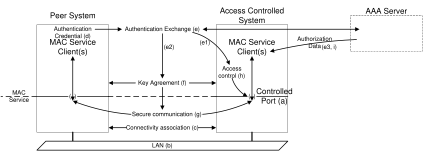
\includegraphics[width=1.0\linewidth]{8021x_fig_6_1_overview.pdf}
    \caption{Schematic overview of an 802.1X controlled Port with MACSec and an external AAA Server\cite{IEEE8021X}.}\label{fig:8021x_fig_6_1_overview}
\end{figure}

Figure \ref{fig:8021x_fig_6_1_overview} shows a high-level overview of an 802.1X enabled port with an external Authentication Server. The exchange of authentication credentials is done between the Peer and an Authenticator using the \ac{EAPOL} protocol and forwarded to an \ac{AAA} server. In the corresponding figure, RADIUS is chosen as the AAA protocol for practical reasons. The \ac{EAPOL} protocol is a Layer 2 protocol for the encapsulation of the \ac{EAP} authentication protocol. According to 802.1X, \ac{EAP} is not mandatory for mutual authentication, and \acp{PSK} may be used instead. Both methods result in a \ac{CAK} used as a root key for the MACSec key agreement protocol. In practice, \ac{EAP} is quite relevant in larger network installations since the flexibility of the protocol allows for a more scalable approach like X509 certificate-based authentication and authentication mechanism that use some kind of centralized directory.

\subsection{EAP and EAPOL}
The \acl{EAP}, as defined in RFC~3748\cite{rfc3748}, is a framework for network-based authentication protocols. As a framework, \ac{EAP} merely defines specific methods for authentication other than an MD5 challenge-response-based, an \ac{OTP}-based and a \ac{GTC}-based method. It is meant to be highly extensible regarding the authentication method, and a large number of methods were proposed since its initial release. While the \ac{EAP} standard itself defines no transport protocol, the 802.1X standard defines the \ac{EAPOL} transport protocol, which encapsulates \ac{EAP} messages in Ethernet frames with the corresponding Ethertype \texttt{0x888E}. \ac{EAPOL} defines four important \ac{EAPOL} \acp{PDU}:

\begin{enumerate}[itemsep=0pt]
    \item \textbf{\ac{EAPOL}-Start}\\
    An \ac{EAPOL}-Start message is sent either by the Supplicant or the Authenticator when the network link becomes available and can be periodically retransmitted until an answer from the other \ac{PAE} is received. This PDU is used to initiate the mutual authentication between the two \acp{PAE}.
    \item \textbf{\ac{EAPOL}-EAP}\\
    The \ac{EAPOL}-EAP \ac{PDU} is used to encapsulate \ac{EAP} messages as defined by RFC~3748. 
    \item \textbf{\ac{EAPOL}-Logoff}\\
    The \ac{EAPOL}-Logoff message is used when a \ac{PAE} wants to terminate the session. When MKA takes place, this type is ignored by the \acp{PAE} to mitigate DOS type attacks.
    \item \textbf{\ac{EAPOL}-MKA}\\
    The \ac{EAPOL}-MKA \ac{PDU} is used to transfer MK\acp{PDU} as defined by IEEE 802.1X. MK\acp{PDU} are used by the \ac{MKA} protocol to select a Key Server and derive cryptographic keys used by MACSec.
\end{enumerate}

EAP, and therefore EAPOL, works in a strict request-response fashion, where each EAP message needs to be acknowledged by the peer system before the next message is sent. This is done by two types of EAP messages: First, the Authenticator sends an \texttt{EAP-Request} messages of type \texttt{Identity} to the Peer. The Peer responses with a message of type \texttt{EAP-Response} that includes an identification string. The Authenticator sends the next message. It includes the requested \ac{EAP} method, which is either acknowledged by the Peer or responded to with a failure indicator if the requested method is not supported. After the Peer sends a successful response, a sequence of method-specific EAP messages is sent back and forth until the method results in a successful authentication or an unrecoverable error. As the last message, the Authenticator sends a status message with the Peer's authentication result.

\section{IEEE 802.1AE}
\begin{figure}[ht]
    \centering
    \includegraphics{8021ae_fig_8_1_macsec.pdf}
    \caption{The MACSec MPDU format\cite{IEEE8021X}}\label{fig:8021ae_fig_8_1_macsec.pdf}
\end{figure} 
The IEEE 802.1AE protocol suite focuses on ``connectionless user data confidentiality, frame data integrity, and data origin authenticity between security associations established by IEEE 802.1X''\cite{IEEE8021AE}. It describes the MACSec \ac{PDU} format and its encryption and integrity protection using the keys established by the MACSec key agreement protocol as described by IEEE 802.1X. MACSec defines a \ac{PDU} format, similar to Ethernet, to transmit frames in a local network that are integrity-protected and protected against eavesdropping through the use of symmetric cryptosystems. IEEE 802.1AE does not have any mandatory dependencies on IEEE 802.1X but is often used in conjunction. In such systems, IEEE 802.1X is used for mutual authentication and the initial key exchange of a single \ac{MSK}. The \ac{MSK} is shared between the Authenticator and the Peer entity. By using the MKA, both entities are now able to perform the \ac{MKA} protocol as an additional symmetric key-exchange protocol to exchange a \ac{LAN}-wide CAK, which is then used by MACSec to send encrypted and integrity-protect \acp{MPDU}. Figure~\ref{fig:8021ae_fig_8_1_macsec.pdf} provides a high-level overview of the \ac{MPDU} format. The MAC addresses are not a part of the \ac{MPDU} itself, but visualize how the format integrates into Ethernet frame-based networks. Instead of the usual Ethernet Ethertype, the Ethertype \texttt{0x885E} is transmitted as a part of the SecTAG format and signals that the following frame  is an \ac{MPDU}. The SecTAG further includes different protocol meta parameters, such as a MACSec internal version number, and whether confidentiality is used or only the integrity feature is used. The SECTag also includes an identifier of the \ac{CA} provided by 802.1X. The secure data field includes user data, which may be protected by symmetric encryption when confidentiality is used. The ICV field includes a cryptographically secured checksum to validate the integrity of the frame. It includes all fields of the \ac{MPDU} as well as the source and destination MAC addresses to protect against spoofing attempts. 


\subsection{MACSec Key Hierarchy}
\begin{figure}[ht]
    \centering
    \includegraphics{8021x_fig_6_3_key_hierachy.pdf}
    \caption{Schematic overview of the MACSec Key Hierarchy\cite{IEEE8021X}}\label{fig:8021x_fig_6_3_overview}
\end{figure}

A shared symmetric key is needed on the Peer systems to provide confidentiality and integrity protection. This key is either a pre-shared secret or results from the authentication. Usually, MACSec requires an EAP method that supports the secure exchange of a 32-byte \ac{MSK} to the client. Figure~\ref{fig:8021x_fig_6_3_overview} shows an overview of the MACSec key hierarchy. The \ac{CAK} serves as a root key, which is not directly used for cryptographic purposes and is either derived from the EAP negotiated \ac{MSK} or from a static pre-shared key. Two further keys, the \ac{ICK} and the \ac{KEK}, are both derived from the \ac{CAK} using a \ac{KDF}. The \ac{ICK} is used to prove possession of the \ac{CAK} and for integrity protection of \acp{PDU}.

The \ac{SAK} is transferred to all members in a \ac{CA} and used for the actual encryption of \acp{PDU} by MACSec. The \ac{SAK} is generated and assigned to members of a \ac{CA} by a Key Server, which is elected by the members of the \ac{CA} using \ac{MKA}. In the case of a pairwise \ac{CAK} directly derived through \ac{EAP}, the role of the Key Server is always fulfilled by the Authenticator. For keys derive through any other method, the Key Server is selected by sending a ``Key Server Priority'' in each MK\ac{PDU}. Participants select the Key Server with the highest priority value. In case of a tie, the Key Server with the highest SCI value is chosen. The SCI value is a combination of the Key Servers MAC address and a numeric port identifier. Multiple Key Servers can generate a group \ac{CAK} to secure the system against the breach of a single \ac{CAK}. To generate the \ac{SAK}, either a strong random number generator on the Key Server or a \ac{KDF} can be used. In the case of distributed \acp{CAK}, each Key Server needs to generate the distributed \ac{CAK} by using a strong random number generator. To preserve the confidentiality of previously transmitted MKA frames, each distributed \ac{CAK} should be independent of any previous generated \ac{CAK} when a new participant joins the \ac{CA}\cite{IEEE8021X}.

\section{Classical Cryptography}


In the following chapters a bi-directional communication between two participants Alice \((A)\) and Bob \((B)\) is assumed. Participants use a cryptographic function \(f_e\) to transfer a cleartext message \(m\) to a ciphertext message \(c\) using a key \(k_e\) and another cryptographic function \(f_d\) to transfer the ciphertext \(c\) back into the cleartext \(m\) using a decryption key \(k_d\). Therefore, \(f_d(f_e(m,k_e),k_d) = m\). In the case of a symmetric cryptosystems, \(k_d = k_e\) holds.

\subsection{Asymmetric Cryptography}

In asymmetric cryptography, the cryptographic key of a participant consists of a private and a public part. The private part of the key is kept secret while the public part is published. To encrypt a message, Alice can use Bob's public key \(B_{k_{pub}}\) to generate a ciphertext. Decrypting the ciphertext is only possible in possession of Bob's private key \(B_{k_{priv}}\). Some digital signature schemes also use asymmetric primitives to provide authentication and integrity protection of the data. To provide a signature of the data, usually, a scheme involving cryptographic hash functions is used. For these schemes, Bob uses his private key to encrypt a hash value of the data. Alice can now use Bob's public key to decrypt the hash sent by Bob and compare it with a hash of the received data. If both hashes are equal, Alice knows with high probability that the hash was generated by the owner of the corresponding private key (e.~g., Bob) and the data were not tempered.

\begin{table}[t]
    \centering
    \caption{Overview of asymmetric key exchange and encryption schemes}

        \begin{tabular}{ l l c }
         \hline
         \textbf{Scheme} & \textbf{Related Problem} \\ 
         \hline
         \ac{RSA} &  Integer Factorization\\  
         Rabin &  Integer Factorization\\  
         \ac{DH} & Discrete Logarithm\\
         Elgamal & Discrete Logarithm \\
         \ac{ECDH} & Discrete Logarithm \\
         \ac{ECDSA} & Discrete Logarithm\\
         \ac{DSA} & Discrete Logarithm \\
    
        \end{tabular}
        \label{table:asymmetric_crypto_schemes}
\end{table}
    
Modern asymmetric (or public-key) crypto schemes rely on the computational complexity to invert certain mathematical functions. Inverting a function is referred to as the computational problem of the underlying cryptosystem, and strong crypto schemes are based on problems that are believed to be intractable. In this context, intractable means that no algorithm exists which can perform this inversion in at least polynomial time. Table~\ref{table:asymmetric_crypto_schemes} shows an overview of modern asymmetric cryptosystems and their underlying problem. It is easy to see that all listed cryptosystems relying on two important primitives. First, the problem of integer factorization, which depends on the complexity of calculating the integer prime factors of a large product \(N\). In RSA, \(N\) and an encryption exponent \(e\) are parts of the public key and therefore available to an attacker. By calculating \(c = m^e \mod N\), Alice can now transform any message into ciphertext. The ciphertext can be converted back into the message with the decryption exponent \(d\), by calculating \(m = c^d \mod N\). To calculate the private key \(d\), an attacker needs to know at least one of the two prime numbers. The second prime can easily be computed by \(x = N/p\). Since the only way to obtain the primes is to factorize the public available parameter \(N\), the cryptosystem's strength depends on the hardness of performing the algorithmic calculation of the (prime-)factorization in a cyclic field.

Another rather important primitive is called the discrete logarithm problem. This problem consists of finding the discrete logarithm \(x\) in a cyclic group \(p\) for \(b^x = a \bmod p \) where \(a\),  \(b\) and \(p\) denote large constants and \(p\) is prime. Instead of a encryption scheme, \ac{DLP}-based schemes like \ac{DH}-based variants, provide the notion of a key exchange protocol, rather than a encryption protocol. Instead of using a static public key for encryption, Alice and Bob are able to calculate a shared secret on-the-fly, using the public available generator \(g\) and a large prime \(p\). For this purpose Alice and Bob can locally compute \(g^a = A\) and \(g^b = B\) for large random numbers \(a\) and \(b\). Now both can exchange \(A\) and \(B\) and calculate \(A^b = C\) and  \(B^a = C\). This holds, because \(A^b = (g^a)^b = (g^b)^a = B^a\). The prime number \(p\) is used to perform all calculation in the cyclic group \(mod p\). An adversary only knows the prime \(p\), the generator \(g\) and both \(A\) and \(B\). To calculate the shared secret \(C\), an adversary need to know either \(a\) or \(b\), which can be found by calculating the discrete logarithm of either \(A\) or \(B\)


Alternatively to the definition of the discrete logarithm problem in finite fields like cyclic groups, a variant defined over elliptic curves is commonly used. An elliptic curve is defined over every point in a finite (Galois) field \(\mathbb{F}_q\) by the function \(E: y^2 = x^3 + ax +b\) with \(a,b \in k \) and \(4a^3 +27b^2 \neq 0\) together with the point of infinity \(\mathcal{O} = (0,1,0)\). The addition of two points and scalar multiplication on that curve is defined, which means that the results of the operations are also located on that curve, with \(\mathcal{O}\) as the neutral element. It is known that the exact definition of these operations, together with the elliptic curve, forms an abelian group. It is now possible to build a key exchange protocol on top of this structure analogous to the original \ac{DH} key exchange protocol by replacing the operations of modular exponentiation in a cyclic group with scalar multiplications and additions on the curve. A benefit of using elliptic curves over classical Diffie-Hellman is that the computational complexity of calculating the discrete logarithm problem on an elliptic curve grows linear instead of logarithmic growth in the classical variant. This allows the same security guarantees by using much smaller key sizes. Further, this allows the implementation of ephemeral \ac{DH} protocols that use a short-lived key, valid only for a single session, and therefore provides the cryptographically desirable notion of forward-secrecy.

As for today, all known algorithms that can solve these problems need at least subexponential time for a valid solution and breaking these schemes, therefore, is impractical, given sufficiently large problem space.

\subsubsection{\texorpdfstring{\acs{KEM}}{KEM} and \texorpdfstring{\acs{KEX}}{KEX}}
Two important terms that need further definition are \ac{KEX} and \ac{KEM}. Both are sometimes ambiguously used in literature. A \ac{KEX} is a protocol that allows Alice and Bob to agree on a shared cryptographic key by exchanging public, non-encrypted messages. An attacker is not able to retrieve the shared secret by intercepting these messages, while Alice and Bob can compute a shared key depending on some secret information in combination with the exchanged messages. An example of a \ac{KEX} is the \ac{DH} key exchange. A \ac{KEM} is a cryptographic protocol that uses an asymmetric scheme to confidentiality transfer a randomly generated secret from Alice to Bob or vice-versa. The public key of one party is used to encrypt the key, which then can be sent over a public channel to be decrypted by the party that possesses the corresponding private key. Both notions are tightly coupled and result in the mutual agreement on a single shared key, which can be used for further symmetric encryption.

\subsubsection{\texorpdfstring{\acf{PFS}}{PFS}}

In classical key exchanges like \ac{RSA}, a single long-term key pair is used for a large number of sessions. This results in a security risk. When the long-term key is compromised, it allows an attacker to decrypt already recorded key-exchanges subsequently. To avoid this problem, the notion of forward-secrecy or perfect forward-secrecy is employed. In a cryptosystem that supports forward-secrecy, an ephemeral key is used, which is only generated for a single session and not stored on any of the participants. A long-term key may still be required to sign the ephemeral key and avoid man-in-the-middle attacks, but this key needs to be independent of the exchanged keying material. Historically, ephemeral keys were no option since cryptosystems like \ac{RSA} requires too much overhead on key generation to use a distinct \ac{RSA} key pair for each session. With the development of more lightweight key exchange protocols like \ac{DH} and Elgamal, ephemeral key exchanges became more practical and are the de-facto standard and many modern cryptosystems like TLS.

\subsection{Symmetric Cryptography}

Unlike in asymmetric schemes, symmetric cryptosystems require Alice and Bob to use the same key for de- and encrypting a message. Applying the key to any plaintext yields the corresponding ciphertext. Applying the same key on the ciphertext again transfers the message back into the original plaintext. Two common distinctions for symmetric crypto schemes are whether the scheme is a so-called block or stream cipher. Stream ciphers are applied on a constant stream of bits, where block ciphers only encrypt blocks of a certain length and therefore may rely on some sort of padding of the small messages to match the block size. A common benefit of symmetric schemes is the performance that can be magnitudes of orders faster as with asymmetric schemes. Therefore cryptosystems like TLS often rely on asymmetric schemes solely to bootstrap a symmetric key between the participants, which is then used to encrypt the actual messages. A typical example of a secure and straightforward implementation of a symmetric cipher is \acl{OTP}. A simple \ac{OTP} implementation uses the XOR function and a pseudo-random number generator, seeded by the symmetric key, to provide a constant stream of keying material. The best-known attacks on such schemes are brute force type of attacks, where the attacker tries to guess the correct key. The security of such schemes, therefore, directly depends on the size of the keyspace.

\section{Post Quantum Cryptography}

With the rise of new quantum computing algorithms like Shor's and Grover's algorithm and the constant improvements of practical quantum computers, the field of \ac{PQC} gained a lot more relevance in recent years. This section will give an introduction to both algorithms and their application. Further, the ongoing \ac{NIST} standardization project for a suitable \ac{PQ} algorithm is discussed.


\subsection{Shor's Algorithm}

Instead of providing an algorithm that can be used to factorize arbitrary integers directly, Shor provides an algorithm that constructs an \ac{FFT} on a quantum computer in polynomial time. Shor uses this \ac{FFT} to calculate the order \(r\) of an element \(x\) in a multiplicative group \(G\) with the generator \(n\). This can be used by choosing a random element of this group and calculate the corresponding order. Afterwards, the greatest common divisor \(\gcd(x^{r/2},n)\) can be calculated which happens to be non trivial divisor of \(n\) if \(r\) is even and \(x^{r/2} \not\equiv -1 \pmod{n} \) holds. Due to the randomization, this yields a factor of \(n\) with a probability of \(\frac{1}{2}\) assuming two distinct prime factors for \(n\). Calculating the other prime factor is now a trivial division. For calculating the greatest common divisor, the Euclidean algorithm can be used, which can be implemented in polynomial time. The algorithm that builds the \ac{FFT} quantum gate also uses only polynomial time, resulting in an overall polynomial runtime for the factorization\cite{shor1999polynomial}.

Shor further shows in his work that the same algorithm for the quantum \ac{FFT} can be applied to solve the discrete logarithm problem as used in Diffie-Hellman based protocols. Since instances of \ac{ECDH} can be reduced to ordinary instances of the discrete logarithm problem in cyclic groups, this efficiently results in a polynomial-time algorithm for both the discrete logarithm problem for cyclic groups and elliptic curves.

\subsection{Grover's Algorithm}

In 1996 Grover published his work on a quantum algorithm that solves the problem of searching an element in an unsorted database with \(n\) elements in \(\bigo(\sqrt{n})\) steps. For any known classical algorithm, the time to find such an element would require \(\bigo(n)\) steps. It is commonly believed that no classical algorithm exists to solve this problem in less time. Bennett et al. proved in their work that the lower bound on any quantum computer is \(\bigo(2^{n/2})\)\cite{bennett1997strengths}, which makes Grover's algorithm within a constant time factor of an optimal solution. Grover uses a unitary matrix that implements a quantum oracle function \(f: \{0,1\}^* \to \{0,1\}\) on a superposition over all possible inputs. This oracle function is used to map the set of possible inputs to 1 if the input value would result in the required output. An example of such an oracle function would be a function that implements a hash function like SHA1 and would output 1 if the hash function's input is equal to the searched value. Grover proves in his work that the algorithm yields the desired element with a probability of \(\bigo(1)\)\cite{grover1996fast}. This has some implications for symmetric cryptosystems as described above since a brute force attack on the key can be interpreted as such a search, where the database is the complete keyspace of size \(2^n\) and the searched element is the symmetric key. Grover's algorithm, therefore, effectively weakens the security of the used cryptosystem by a quadratic factor.

\section{Post-Quantum Cryptography Standardization}
With respect to Shor's algorithm and the possibility of practical applications in the foreseeable future, the \ac{NIST} started a standardization project in December 2016 to decide on ``one or more additional public-key cryptographic algorithms to augment \ac{FIPS} 186-4, Digital Signature Standard (DSS), as well as special publications SP 800-56A Revision 2''\footurl{https://csrc.nist.gov/news/2016/public-key-post-quantum-cryptographic-algorithms}\footurl{https://csrc.nist.gov/publications/detail/fips/186/4/final}. The goal of this project is to provide a quantum-resistant, asymmetric crypto and signature scheme that can be used additionally or as an alternative to the currently specified algorithms that are affected by the work of Shor and the ongoing improvements of practical quantum computers. The initial call for submissions ended on November 30, 2017. The evaluation process is grouped into multiple rounds, where comments from the public and an ongoing discussion on the proposed algorithms are used to refine the selection of several acceptable cryptosystems for standardization. As for today, the project is currently in the third, and therefore final round of evaluation.


\begin{table}[ht]
    \centering
    \caption{Overview of the defined security level}
        \begin{tabular}{cll}
        \hline
         \textbf{Level} & \textbf{Primitive} & \textbf{Reference} \\
         \hline
         1 &  128-bit Block Cipher Key Search & AES128 \\
         2 &  256-bit Hash Function Collision & SHA256, SHA3-256 \\
         3 &  192-bit Block Cipher Key Search & AES92 \\
         4 &  384-bit Hash Function Collision & SHA384, SHA3-384 \\
         5 &  256-bit Block Cipher Key Search & AES256 \\
        \end{tabular}
        \label{table:nist_security_level}
    \end{table}


The call for submissions defines multiple so-called security levels. Each level is defined by a reference primitive and each submission is compared to one or more of these security levels. Submissions often define different parameter selection to match different security levels. The reference algorithms, as shown in Table~\ref{table:nist_security_level}, are well-studied crypto algorithms that can be used for ease of comparison with the submitted algorithms. Further, the following properties are defined as desirable:

\begin{enumerate}
    \setlength{\itemsep}{0pt}
    \item Perfect forward-secrecy
    \item Resistance to side-channel attacks
    \item Resistance to multi-key attacks
    \item Resistance to misuse
\end{enumerate}

All algorithms provide IND-CCA guarantees, while some algorithms also provide an IND-CPA compliant instance. The IND notation stands for ciphertext indistinguishability and is defined as an experiment where an attacker sends two chosen-plaintext messages of equal length to a challenger party with access to an encryption function \(E\) and a decryption function \(D\) seeded by an encryption key \(K_e\) and a decryption key \(K_d\). The challenger party decides to encrypt one of the two messages randomly, and the attacker tries to guess which of the chosen plaintext messages resulted in the returned ciphertext. The experiment further includes an encryption and decryption oracle, available to the attacker to encrypt and decrypt arbitrary messages under certain conditions.

\begin{itemize}
    \item \textbf{\ac{IND-CPA}} \\
    In this setting, the attacker is allowed a single iteration, i.~e., send two plaintext messages to the challenger and then have to decide which message results in the returned ciphertext. The attacker is further allowed to issue additional computations in polynomial time, including calls to the encryption oracle, before sending the plaintext and after receiving the ciphertext. These guarantees are needed to limit the attacker to computations in polynomial time.
    \item \textbf{\ac{IND-CCA}}
    In this setting, the attacker is further allowed to make arbitrary calls to a decryption oracle before sending the message to the challenger while keeping the restriction on a polynomial number of steps. This allows the attacker multiple iterations of calls to the encryption oracle and implies that multiple iterations do not weaken the cryptographic protocol.
    \item \textbf{\ac{IND-CCA2}}
    In this setting, the attacker is now additionally allowed to call the decryption oracle after he received to ciphertext from the challenger, with the only exception that the attacker is not allowed to send the received ciphertext itself to the oracle. This setting implies that an attacker has no additional advantage by using the decryption oracle after knowing the ciphertext that corresponds to one of the messages.  
\end{itemize}

Round 3 of the \ac{NIST} PQ project evaluates submissions under the guarantees provided by \ac{IND-CCA} with up to \(2^{64}\) queries to the oracle. This is useful for algorithms that depend on key re-usage and therefore require long-term security of the used keys. It is further allowed to submit additional cipher specifications that only provide \ac{IND-CPA} guarantees, with restrictions on the re-usage of a single key. This may be beneficial for schemes that have significant performance advantages under \ac{IND-CPA}.



\subsection{Public-key Encryption and Key-establishment Algorithms}

\begin{table}[ht]
    \centering
    \caption{\ac{NIST} Round 3 Candidates for asymmetric \ac{KEM} and \ac{KEX} algorithms. Candidates are either finalists or alternate candidates. Finalists are the preferred candidates by the \ac{NIST} and only minor changes are expected, while alternate candidates may be subject to more significant changes.}
    \begin{tabular}{llc}
            \hline
            \textbf{Background} & \textbf{Scheme} & \textbf{Finalist} \\
            \hline
            \multirow{3}{*}{Code-Based} 
            & BIKE & --- \\
            & Classic McEliece & \cmark \\
            & HQC & ---\\
            \hline
            \multirow{5}{*}{Lattice-Based} 
            & SABER & \cmark\\
            & CRYSTALS-KYBER & \cmark \\
            & NTRU & \cmark \\
            & NTRU Prime  & ---\\
            & FrodoKEM & --- \\
            \hline
            Isogeny-Based & SIKE & ---\\
            \hline
        \end{tabular}
    \label{table:nist_round_2_kem}
\end{table}

One part of the \ac{NIST} project is selecting one or more public key encryption or key encapsulation methods. Table~\ref{table:nist_round_2_kem} shows the currently discussed candidates, grouped by their mathematical foundation. In the remainder of this section, an introduction to the mathematical problems and their application for asymmetric cryptography is given.

\subsubsection{Lattice-based Key Exchange}

\begin{figure}[ht]
    \centering\includegraphics[width=1.0\linewidth]{plot_scatter_lattice_based_latency_pubkeysize.pdf}
    \caption{Overview of the current lattice-based Round 3 candidates of the \acs{NIST} \acs{PQ} standardization project. Only parameter selections with ING-CCA guarantees are shown. The x-axis shows the average latency for key generation, encapsulation and decapsulation of a shared secret in \acs{CPU} cycles on a logarithmic scale. The y-axis shows the public key size in bytes on a logarithmic scale. Benchmark results are part of eBACS\cite{eBACS}}\label{fig:lattice_level3_scatter}
\end{figure}

Lattice-based cryptosystems are based on the mathematical foundation of so-called lattices. A lattice is an n-dimensional geometric space with a periodical structure, described by a set of \(n\) linearly independent basis vectors \(b_1, \dots, b_n \in \mathbb{R}^n\), known as the basis \(B\) of a Lattice \(\mathcal{L}\). The lattice consists of points that are described by any linear combination of these vectors. The security of lattice-based systems depends on the hardness of multiple problems in these lattices\cite{micciancio2009lattice}.

\begin{enumerate}
    \setlength{\itemsep}{0pt}
    \item \ac{SVP} Find the shortest non-zero vector for a given basis \(B\)
    \item \ac{CVP} For a given basis \(B\) and a vector \(t\), find the lattice point closest to \(t\)
    \item \ac{SIVP} For a given basis \(B\) find a set set \(S\) of linearly independent vectors in \(\mathcal{L}(B)\) that minimize the quantity \(\Vert S \Vert = \max_i(\Vert s_i \Vert)\)
\end{enumerate}

Most lattice-based cryptosystems are not based on an exact solution to these problems but instead, use a variant where the solution needs to be within an approximation factor \(\gamma\). The best-known algorithms to solve these problems are running within polynomial time and give an approximation within an exponential factor. For an exact solution or a solution with an approximation factor within a polynomial factor, the best-known algorithms require exponential running time and space, making them impractical for a certain size for \(n\)\cite{micciancio2009lattice}. It is believed that there may be no algorithms that solve the \ac{SVP} in polynomial running time within a polynomial approximation factor. This hardness can be used to build cryptographic systems on top of these problems. Ajtai was the first that recognized the implication of lattice for cryptographic purposes by designing a one-way, collision-resistant hash function that can be reduced to the worst-case hardness of the \ac{SVP}\cite{ajtai1996generating}. In this context, worst-case hardness means that breaking these cryptosystems is at least as hard as breaking any \ac{SVP} instance within polynomial bounds, in polynomial time. Later, other cryptosystems were proposed on the foundation of Ajtai's work, including multiple public-key cryptosystems. As for now, lattice-based public-key cryptosystems seems to be a trade-off between practicability and proven security. Multiple proposed systems provide a desirable property of provable security by the cost of rather large key sizes. For example, a cryptosystem proposed by Ajtai and Dwork~\cite{ajtai1997public} with a worst-case hardness guarantee implies key sizes of serval gigabytes for lattices with a dimensional size up to ``serval hundreds''\cite{micciancio2009lattice}. Again, in this case, worst-case hardness means that breaking the system implies an efficient algorithm for any instance of the underlying lattice problem.

One instance of lattice-based public-key cryptosystems for which no such proof exists but which can be implemented efficiently and with practical key sizes is called NTRU. NTRU is a probabilistic cryptosystem, which means that it introduces some randomness into the encryption process and therefore results in many possible ciphertexts for a given plaintext\cite{hoffstein1998ntru}. The original description of NTRU is based on classical ring-based polynomial algebra but can also be given in the context of lattices. Another interesting class of lattice-based cryptosystems is based on the \ac{LWE} problem. The learning with error problem is a search problem which consists of finding a secret n-dimensional vector \(s \in Z_q^n\), given a polynomial number of vectors \(x_i \in Z_q^n\), where each vector is generated by sampling a random vector \(a_i \in Z_q^n \) and calculating the inner product \(b_i = \langle a_i, s \rangle \) and finally adding some noise by calculating \(x_i = b_i + r_i\) where \(r_i \in Z_q\) is sampled from a probability distribution. There is also an equivalent decision problem with the task to distinguish whether the set of noisy vectors is either completely randomly sampled from a uniform distribution or the result of the inner product combination, as shown above. It is shown that the search LWE problem can be reduced to a lattice-based approximate-\ac{SVP} and approximate-\ac{SIVP} by using a reduction algorithm that involves a quantum computer. That implies that an algorithm that solves these kinds of problems in polynomial time would provide a polynomial-time quantum algorithm that solves the approximate-\ac{SVP}.

On the other hand, this proof does not imply that the same hardness guarantees also holds for all classical algorithms. While cryptosystems based on the LWE problem provide better hardness guarantees that classical lattice-based cryptosystems like NTRU, the needed space to store the public key is still rather big compared to classical cryptosystems but still considered practical\cite{micciancio2009lattice}. A parameter selection of all Round 3 candidates with their latency and public key sizes is shown in Figure~\ref{fig:lattice_level3_scatter}. Except for \texttt{FrodoKEM}, all shown algorithms use public key sizes of a few KB. The main difference in Figure~\ref{fig:lattice_level3_scatter} are the \acs{CPU} cycles needed to generate a key pair and to encapsulate and decapsulate a shared secret. Depending on the algorithm, the differences are between a few orders of magnitude.

\subsubsection{Code-based Key Exchange}
\begin{figure}[ht]
    \centering\includegraphics[width=1.0\linewidth]{plot_scatter_code_based_latency_pubkeysize.pdf}
    \caption{Overview of the current code-based Round 3 candidates of the \acs{NIST} \acs{PQ} standardization project. Only parameter selections with ING-CCA guarantees and \acs{NIST} security level 3 are shown. The axes are displayed on a logarithmic scale. The x-axis shows the average latency for key generation, encapsulation and decapsulation of a shared secret in \acs{CPU} cycles on a logarithmic scale. The y-axis shows the public key size in bytes on a logarithmic scale. Benchmark results are part of eBACS\cite{eBACS}}\label{fig:code_level3_scatter}
\end{figure}

Code-based cryptography is another promising candidate for \ac{PQC}. Cryptosystems in this category utilize the hardness of certain problems that arise from coding theory, which focuses on the design and algorithmic implementation of error detection and correction codes. The first proposal for a coding theory based public-key cryptosystem was designed by MCEliece in 1976. MCEliece uses a class of \ac{ECC} called general binary Goppa codes. The design relies on the fact that binary Goppa codes can be decoded efficiently, while no algorithm for general linear codes exists. McEliece uses this property to hide a Goppa code in a general linear code by randomly generating two matrices to transfer the matrix for the Goppa code into a matrix for a general linear code with the same distance and error rate as the original Goppa code. This matrix can be used as the public key, while the randomly generated matrices are used as the private key. A message can be encrypted by encoding the message into a code word in the general linear code and applying random errors to the resulting code word. To decrypt the message, an attacker needs to decode the general linear code and correct the random error, which is known to be NP-complete and for which no polynomial-time algorithm is believed to exists\cite{berlekamp1978inherent}. Alternatively, an attacker could restore the structure of the original generator matrix and decode the code word efficiently. While there are \ac{ECC} for which such an attack is possible, there is no such attack currently known for Goppa codes. With the knowledge of the two permutation matrices, it is computationally easy to transfer the message back into a binary Goppa code. By applying Peterson's algorithm, it is now possible to correct the random error and decode the code word back into the original message in polynomial time\cite{mceliece1978public}. Besides being released over 40 years ago, the original description by McEliece remains nearly unbroken in terms of that it provides nearly the same security level of \(2^{64}\) binary operations to break an instance of the cryptosystems with the parameters from the original paper. An attack first described by Canteaut and Sendrier\cite{canteaut1998cryptanalysis} and later refined by Bernstein et al.\cite{bernstein2008attacking} was able to reduce this value only to \(2^{60.55}\) while still using the parameters originally proposed by MCEliece. On the downside, the McEliece cryptosystem needs rather large public keys, ranging from multiple KB to a few MB. Multiple variants of Code-based cryptosystems were proposed in the past, using different types of codes or depending on different primitives to provide improvements in terms of the public key sizes. A parameter selection of all Round 3 candidates with their latency and public key sizes is shown in Figure~\ref{fig:code_level3_scatter}. Bike and the HQC scheme, which both rely on quasi-cyclic \acp{ECC}, are both able to provide better performance and key sizes than classic MCEliece.


\subsubsection{Isogeny-based Key Exchange}

\begin{figure}[ht]
    \centering\includegraphics[width=1.0\linewidth]{plot_scatter_isogeny_based_latency_pubkeysize.pdf}
    \caption{Overview of the current implementations of the SIKE Round 3 candidates of the \acs{NIST} \acs{PQ} standardization project. All parameter selections that correspond to different security levels are shown. The x-axis shows the average latency for key generation, encapsulation and decapsulation of a shared secret in \acs{CPU} cycles. The y-axis shows the public key size in bytes. Benchmark results are part of eBACS\cite{eBACS}}\label{fig:sike_scatter}
\end{figure}

Instead of residing in completely new mathematical foundations for asymmetric cryptography, isogeny-based cryptographic protocols are located in the well-established field of \ac{ECC}. As for all problems which depend on the computational hardness of the discrete logarithm problem both, the cyclic group based \ac{DH} and \ac{EC}-based protocols are affected by Shor's algorithm and therefore are broken by a universal quantum computer. Isogeny-based \ac{EC} cryptography aims to solve this problem while still relying on elliptic curves, providing small public key sizes and allowing for ephemeral key exchanges. An isogeny \(\phi\) is a surjective mapping between two elliptic curves, such that that \(\phi\) is a group homomorphism. Another class of mappings between elliptic curves that is also a group homomorphism is called an isomorphism. An isomorphism is a bijective map between two elliptic curves. Two elliptic curves are isomorphic if and only if they have the same j-invariant. The j-invariant of an elliptic curve \(E \) is defined as \(j(E) = 1728 \frac{4a^3}{4a^3 +27b^2}\). Two j-invariant are isogenous if there exists an isogeny between the corresponding elliptic curves. It is now possible to view these isogenies as a graph. The vertices are a set of elliptic curves, described by their j-invariant and the edges represent the isogenies that map these j-invariants. These graphs are undirected since for every isogeny that maps \(E \to E'\); there is a corresponding isogeny that maps \(E' \to E\). Assuming an elliptic curve \(E\) defined over a finite field \(k\) with characteristics \(p\). For any prime \(l \neq p\) there exists \(l+1\) distinct isogenies of degree \(l\). This results in \(l+1\) edges for every vertex in the graph. These graphs are so-called expander graphs. Random walks on such expander graphs of a length close to the graph's diameter results in any vertex of the graph with a probability close to uniform. This random property can be used to build a cryptosystem on top of such graphs. In such a cryptosystem, both Alice and Bob generate two distinct isogeny graphs of degree \(l\), called \(l_A\) and \(l_B\) for a public curve \(E\). Now, both parties take a random walk in their respective graph of a certain length, depending on some large exponent \(e\). This results in two cyclic subgroups \(A, B \subset E\) with bases \(\langle P_A, Q_A \rangle\) and \(\langle P_B, Q_B \rangle\). Afterwards, both party publish \(A/ \langle E \rangle \) and \(B/ \langle E \rangle \), generated by their secret isogenies \(\alpha: E \to E/\langle A \rangle \) and \(\beta: E \to E/ \langle B \rangle\). For an attacker, it is a hard problem to calculate \(\alpha\) and \(\beta\) given \(E/ \langle A \rangle\) and \(E/ \langle B \rangle\), while there are efficient algorithms available to calculate the isogeny, given both curves. Additionally, Bob publish the values \(\beta(P_A)\) and \(\beta(Q_A)\). This allows Alice to generate \(\beta(A) E \to (E/\langle A \rangle)/ \langle B \rangle\) and vice-versa allows Bob to calculate \(\alpha(B) E \to (E/ \langle B \rangle )/A\). Since, \((E/ \langle B\rangle )/ \langle A \rangle\) and \((E/\langle A \rangle)/ \langle B \rangle\) are isomorphic, they share the same invariant which therefore can be used as a shared secret\cite{DBLP:journals/corr/abs-1711-04062}. Figure~\ref{fig:dh_dlog_isogeny} shows a simplified overview of the link between the key agreement in classical DH based protocols and the isogeny based variants. Both systems use an elliptic curve as a common base and communicate some public parameters. A combination of the private information, combined with the public parameters, results in a shared secret \(g^{ab}\) and \( E / \langle A, B \rangle\), respectively.

\begin{figure}[!ht]
    \centering
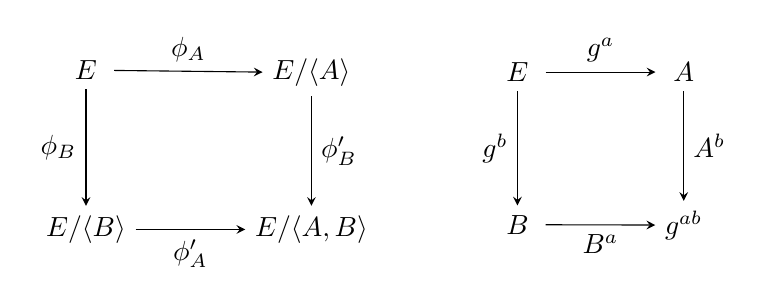
\begin{tikzpicture}[auto,node distance=1.3cm]
    \begin{scope}
        \matrix (m) [matrix of math nodes,
        row sep=4em,
        column sep=4em,
        minimum width=2em] {
        E                     & E / \langle A \rangle    \\
        E / \langle B \rangle & E / \langle A, B \rangle \\
        };
        \path[-stealth]
        (m-1-1) edge node [above] {$\phi_A$}  (m-1-2)
        (m-1-1) edge node [left]  {$\phi_B$}  (m-2-1)
        (m-2-1) edge node [below] {$\phi_A'$} (m-2-2)
        (m-1-2) edge node [right] {$\phi_B'$} (m-2-2);
    \end{scope}

    \begin{scope}[xshift=5cm]
        \matrix (m) [matrix of math nodes,
        row sep=4em,
        column sep=4em,
        minimum width=2em] {
        E                     & A    \\
        B &  g^{ab}\\
        };
        \path[-stealth]
        (m-1-1) edge node [above] {$g^a$}  (m-1-2)
        (m-1-1) edge node [left]  {$g^b$}  (m-2-1)
        (m-2-1) edge node [below] {$B^a$} (m-2-2)
        (m-1-2) edge node [right] {$A^b$} (m-2-2);
    \end{scope}
\end{tikzpicture}
\caption{High level overview of classical \ac{DH} on the right and isogeny based \ac{DH} on the left\cite{TikZ:for:Cryptographers}.}\label{fig:dh_dlog_isogeny}
\end{figure}

Due to their analogous behavior to related \ac{DH} type protocols, this class of algorithms is called \ac{SIDH}. The only instance of such key exchanges currently enlisted in the \ac{NIST} \ac{PQ} project is called SIKE. Figure~\ref{fig:sike_scatter} shows the currently proposed ciphers with different parameter selections to match certain security levels.

\subsection{Digital Signature Algorithms}

\begin{table}[ht]
    \centering
    \caption{\ac{NIST} Round 3 Candidates for \ac{DSS} algorithms}
    \begin{tabular}{llc}
            \hline
            \textbf{Background} & \textbf{Scheme} & \textbf{Finalist} \\
            \hline
            \multirow{2}{*}{Lattice-Based} 
            & CRYSTALS-DILITHIUM & \cmark\\
            & FALCON & \cmark \\
            \hline
            \multirow{2}{*}{Multivariate} 
                & GeMSS & \xmark\\
                & Rainbow & \cmark \\
            \hline
            Zero-Knowledge Proof & Picnic & \xmark \\
            \hline
            Hash-Based & SPHINCS+ & \xmark \\
            \hline
        \end{tabular}
    \label{table:nist_round_2_dss}
\end{table}

In addition to the mentioned public-key encryption and key-establishment algorithms, the \ac{NIST} \ac{PQ} project also focuses on a replacement for the currently used digital signature schemes. In practice, most of these schemes also rely on cryptographic protocols like \ac{RSA}, \ac{DH} or \ac{ECDH} and therefore are weakened by Shor's algorithm. Table~\ref{table:nist_round_2_dss} shows an overview of the currently discussed Round 3 candidates, grouped by their underlying mathematical primitives.

\subsubsection{Lattice-based Signatures}

\begin{figure}[!ht]
    \centering\includegraphics[width=1.0\linewidth]{plot_scatter_lattice_signlatency_signsize.pdf}
    \caption{Overview of the current implementations of lattice-based signature schemes in Round 3 of the \acs{NIST} \acs{PQ} standardization project. The y-axis shows the latency to sign a 59 Byte message in \acs{CPU} cycles. The x-axis shows the size of a signature for a 23 Byte message. The size of the markers reflects the relative size of the public keys. The color encodes the stated security level. Benchmark results are part of eBACS\cite{eBACS}}\label{fig:lattice_sign_scatter}
\end{figure}

Lattice-based schemes work on the foundation of lattice-based cryptography, as described in the last section. For \texttt{Dilithium}, a Fiat-Shamir construction is used to generate a non-interactive signature scheme from an interactive zero-knowledge proof. In general, such schemes work in a request-response fashion, where a challenger request proof from another party whether this party is the owner of a secret key, given the corresponding public key, without leaking information about the secret key. In an interactive setup, communication between both parties is required. However, there is a technique called Fiat–Shamir heuristics that allows implementing a non-interactive digital signature scheme by replacing the interactive request from the challenger with a cryptographic hash function over the message that needs to be signed. Initially, these schemes were designed for the \ac{RSA} cryptosystem\cite{fiat1986prove}. \texttt{Dilithium} is founded on a variation of this technique called Fiat-Shamir with aborts, which works for lattice-based systems. Since naive Fiat-Shamir-based implementations would leak information about the private key, assuming the signature is in a certain numerical range, this scheme allows the challenged party to abort a verification process if the resulting computation results in such a leak. The challenging party must restart the verification process until a valid signature is generated. The number of iterations depends on the probability of receiving a malicious random challenge that would result in a leak. In the original work by Lyubashevsky, the probability for a failure is a small constant of about \(2/3\). Therefore, only a small number of iterations is required until a successful signature is created. For one-time signatures, the same transformation can be applied. The signing party only needs to create valid signatures until a signature in the desired range is generated and then can continue to publish this signature, without the need of publishing the failed attempts\cite{10.1007/978-3-642-10366-7_35}.

In the case of \texttt{FALCON}, the signature scheme is based on one-way trapdoor permutation in lattices as described by Gentry, Peikert and Vaikuntanathan\cite{cryptoeprint:2007:432}. This construction uses a hash and sign scheme, where a message is hashed and encrypted by a lattice-based encryption function using the private key. The encryption function results in a vector in the lattice close to the hash value of the message. The distance between the pre-image of the message and the resulting vector can be used as a signature. To verify this signature, a challenger only needs to prove that the signature value is short (i.~e., close to the pre-image) and that the decrypted value is equal to the hashed value of the message.

The benefits of lattice-based schemes are the fast signature latencies and acceptable signature sizes. However, both come with the cost of rather large public keys. Figure~\ref{fig:lattice_sign_scatter} shows an overview of the different algorithms. \texttt{FALCON} places special focus on the combined sizes of the signatures and the public keys since both are usually needed to be transmitted in a certificate-based authentication setting. The plot shows that it achieves both goals compared to \texttt{Dilithium} and even outperforms all \texttt{Dilithium} designs in terms of signature size, even at the highest available security level.


\subsubsection{Multivariate-based Signatures}
\begin{figure}[ht]
    \centering\includegraphics[width=1.0\linewidth]{plot_scatter_mv_signlatency_signsize.pdf}
    \caption{Overview of the current implementation of multivariate signature schemes in Round 3 of the \acs{NIST} \acs{PQ} standardization project. The y-axis shows the latency to sign a 59 Byte message in \acs{CPU} cycles on a logarithmic axis. The x-axis shows the size of a signature for a 23 Byte message. The size of the markers reflects the relative size of the public keys in KB. The color encodes the stated security level. Benchmark results are part of eBACS\cite{eBACS}}\label{fig:multivariate_sign_scatter}
\end{figure}

Multivariate signature schemes are based on the notion of multivariate cryptography. Multivariate crypto schemes are candidates for a \ac{PQ} key-exchange mechanism, and a few examples of such cryptosystems were part of the first round of the \ac{NIST} \ac{PQ} project. Since the \ac{NIST} had concerns regarding the full security of such systems, no multivariate key exchange advanced to the second round. However, they are still used as parts of multiple signature schemes. In general, multivariate cryptosystems are asymmetric cryptosystems that depend on the hardness of solving multivariate polynomials over a finite field, which is proven to be NP-complete. In a simplified design, based on a system called \ac{HFE}, the cryptosystem uses a finite field \(F_q\) of cardinality \(q\) and prime characteristics \(p\). Usually  \(p = 2\) is used. A polynomial \(f(x) = \sum_{i,j} \beta_{ij}x^{q^{\theta{ij}} + q^{\varphi{ij}}} + \sum_{k} a_{k} x^{q^{\epsilon_{k}}} + \mu \in F_{q^n}[x]\) for some random integers \(\varphi{ij}, \theta{ij}, \epsilon_{k} \geq 0 \), together with two affine transformation \(s, t: (F_q)^n \to (F_q)^n\) is chosen as the private key. A message \(x\) can be transformed to ciphertext by applying \(t(f(s(x))) = p_1(x_1, \dots, x_n) , \dots, p_n(x_1,\dots,x_n) \), where \(p_i\) are quadratic polynomials. Given \(f, t, s\) the polynomials \(p_i\) can be computed efficiently. The polynomials act as the public key and computing \(f, t, s\) given the public key corresponds to a hard problem\cite{patarin1996hidden}. Alternatives to this scheme are the  ``balanced oil and vinegar'' and the ``unbalanced oil and vinegar'' schemes. In balanced oil and vinegar systems, the secret key consists of a set of \(n\) equations that satisfy a certain structure. Each equation consists of secret coefficients, a number of \(n\) oil variables and a number of \(v\) vinegar variables. It is important that the equation does not compute a product of oil and vinegar variables, i.~e., the variables are not ``mixed''. For computing a valid signature, the vinegar variables are chosen randomly, and the oil variables are computed by a gaussian reduction. Both can be done efficiently in practice. The resulting signature can be verified using the public key, a matrix consisting of \(n\) equations that are generated by an affine transformation of the private key. In \ac{HFE} and oil and vinegar schemes, the signatures are valid if all equations in the public key are satisfied by the signature. For balanced systems \(n = v\) holds. However, there is a known attack when the number of oil variables is equal or within a small difference to the number of vinegar variables that allow an attacker to forge arbitrary signatures. \cite{kipnis1998cryptanalysis}\cite{kipnis1999unbalanced} This type of attack can be mitigated by unbalanced systems where \(v >> n\). The authors of \cite{kipnis1999unbalanced} showed that the attack is not applicable for \(v > 2n\) and propose a system with \(v \simeq \frac{n^2}{2} \). Furthermore, they described an algorithm that can efficiently break unbalanced schemes with \(v \geq n^2 \). Rainbow is a signature scheme that uses an unbalanced oil and vinegar construction. A benefit of using such schemes is that they can be implemented very efficiently in practice and provide small signature sizes. Figure~\ref{fig:multivariate_sign_scatter} shows a comparison of different signature schemes build on top of multivariate cryptosystems with respect to signature sizes and latencies. In a system based on the QUARTZ signature scheme, called GeMSS, a combination of the \ac{HFE} cryptosystem and so-called minus and vinegar modifiers are used to build a digital signature scheme. The minus modifier reduces the number of polynomials from the \ac{HFE} system that are published, and the vinegar modifier adds additional vinegar variables to the \ac{HFE} function \(f\). Both steps aim to add additional security to the classical \ac{HFE} notion\cite{patarin2001quartz}.

\subsubsection{Hash-based Signatures}


\begin{figure}[!ht]
    \centering\includegraphics[width=1.0\linewidth]{plot_scatter_hash_based_signlatency_signsize.pdf}
    \caption{Overview of the current implementation of hash-based signature schemes in Round 3 of the \acs{NIST} \acs{PQ} standardization project. All security level 3 implementations are shown. The y-axis shows the latency to sign a 59 Byte message in \acs{CPU} cycles on a logarithmic axis. The x-axis shows the size of a signature for a 23 Byte message. Benchmark results are part of eBACS\cite{eBACS}}\label{fig:hash_sign_scatter}
\end{figure}

Instead of relying on a combination of asymmetric cryptography and cryptographic hash functions, hash-based signatures rely on the security of cryptographic hash functions only. The first construction that uses a hash-based approach was introduced by Lamport in 1979\cite{lamport1979constructing}. In his work, Lamport uses a one-way hash function \(F: \{0,1\}^* \to \{0,1\}^n\), for a fixed value \(n = 2^m\). The security of the system depends on the size of n and is typically in the range of \([128,512]\). First, Alice needs to compute \(n\) key pairs, where each element is a \(n\) bit long randomly generated number. The resulting set of numbers 
\(sk = (\{0,1\}^n)_{0,0}, (\{0,0\}^n)_{0,1}, (\{0,1\}^n)_{1,0}, (\{0,0\}^n)_{1,1}, \dots, (\{0,1\}^n)_{n,0}, (\{0,0\}^n)_{n,1}\) is used as the secret key. The public key consists of the \(n\) bit long hash value for each element \(pk = \{F(sk_i) \vert \forall i \le n \}\). To sign a single message \(m = \{0,1\}^n\), Alice signs each bit \(m_i\) individually by publishing the corresponding pair of the secret key \(x_{i,m_i}\). Bob can now verify the signature by calculating the hash value of each signature bit and compare it to the corresponding hash in Alice's public key. Since this method leaks parts of the secret key, it is obvious that using a single key pair for multiple signatures would allow an attacker to forge arbitrary signatures. Therefore Lamport's original scheme is a one-time signature scheme, meaning that every key pair can only be used to sign a single message. A further downside of this scheme is the rather large key sizes of \(2n^2\). As an alternative to this one-time scheme, multiple many-time schemes were proposed, allowing a single public key for more than a single application up to a fixed number of iterations. These schemes often use binary Merkle hash-trees as a compact data structure with a trade-off in terms of computational complexity. A Merkle tree is built in a bottom-up approach with a fixed number of leaves \(N=2^n\). In a Lamport like signature scheme, each leaf corresponds to a public-private-key pair \((sk_i, pk_i) \) as described above. The root of the hash tree is the newly published public key \(pk\). To sign a single message Alice now needs to publish a valid signature as a result of one \((sk_i,pk_i)\) key pair together with the corresponding one-time public key \(pk_i\) and the values for all \(n\) adjacent nodes that are included in the path from the root to the leaf. Bob can now validate the signature by reconstructing the path in the Merkle tree, using the underlying hash function and the signature, and comparing the result to the public key (i.~e. the root of the tree). The one-time signature leaves are usually used in a specific order from the leftmost to the rightmost leaf, which results in a total of \(N\) possible signatures. The size of the public key is decreased to a single hash value, while the size of the signatures is increased by a constant factor. A downside of this method is the fact that the whole tree needs to be computed upon key generation due to the bottom-up approach. this makes key generation and signature time exponential with respect to the height of the tree (and, therefore, the number of messages that can be signed). Further, this scheme reintroduces some kind of state into the signature process by requiring the signer to use an incrementing key-pair every time a message was signed. A stateless alternative to the data structure was proposed by Goldreich. Instead of a bottom-up tree approach, a top-down certificate tree is used. In this construction, the nodes of the binary tree use hash-based one-time signatures to sign both child nodes. The leaves of the tree correspond to one-time hash-based signatures to sign the actual messages. The secret key acts as a seed to a pseudo-random function to generate the tree ad-hoc. To ensure a single key pair is used only a single time, Goldreich proposed two methods. First, a \(n\) bit hash of the message is used as the index for a tree with height \(n\). This method ensures that a key pair is only used once as long as there is no collision in the used hash function. A downside of this scheme is the need for rather large signatures since the size of a single signature is cubic with respect to the size of the tree. An alternative approach is to select the index of the used leaf randomly. This allowed smaller tree sizes with a certain, negligible probability for key re-usage\cite{bernstein2015sphincs}. Currently, only a single instance of hash-based signature is a candidate for Round 3 of the \ac{NIST} \ac{PQ} project. SPHINCS+ is based on SPHINCS and uses a Goldreich construction with a so-called, few-times signature scheme and a hypertree construction to reduce the sizes of the signatures drastically by increasing the time to sign a single message. Contrary to one-time hash-based signatures, few-time hash-based signatures allow reusing a single public-private key-pair a limited amount of time. In the original design of SPHINCS, the usage of few-time signatures allowed to decrease the height of the tree from \(256\) to \(60\) while maintaining the same post-quantum security guarantees\cite{bernstein2015sphincs}. The usage of a hypertree model for the Goldreich tree allowed a further reduction of the signatures sized by increasing signature time exponentially with respect to the number of layers used in the hypertree. Figure~\ref{fig:hash_sign_scatter} shows an overview of the different SPHINCS+ implementations. All algorithms are implemented as an s-variant (size) and an f-variant (fast), optimized either for signature sizes or signature time.

\subsubsection{Zero-Knowledge-Proofs on Arbitrary Circuits}

\begin{figure}[!ht]
    \centering\includegraphics[width=1.0\linewidth]{plot_scatter_zk_signlatency_signsize.pdf}
    \caption{Overview of the current implementation of ZK-based signature schemes in Round 3 of the \acs{NIST} \acs{PQ} standardization project. All security level 3 implementations are shown. The y-axis shows the latency to sign a 59 Byte message in \acs{CPU} cycles on a logarithmic axis. The x-axis shows the size of a signature for a 23 Byte message. Benchmark results are part of eBACS\cite{eBACS}}\label{fig:zk_sign_scatter}
\end{figure}

As in hash-based signature schemes, ZK-proofs on arbitrary circuits based schemes use symmetric, polynomial-time computable primitives such as the SHA or AES function families to prove to a challenging party \(V\) that the proving party \(P\) knows some secret \(x\) without revealing information about the secret itself. In a system called ZKBoo, this works by interpreting the symmetric primitive as a binary relation \(R \subset \{0,1\}^* \times \{0,1\}^*\), where the result of the computation is a relation of the inputs to the output of the symmetric primitive e.~g. \( R = \{(x,y) \vert y = SHA(x)\}\). The language L is the set of \(x\) variables for a given \(y\) that results in a ``yes'' answer (e.~g. \(R(x,y) = 1\))\cite{giacomelli2016zkboo}. When looking at SHA1 as an example, the language L is the set of all tuples \((x,y)\) that result in some hash value \(y\) for all possible inputs \(x\). In this protocol, the proofer \(P\) wants to convince a verifier \(V\) that he knows an instance \(l \in L\), without revealing the associated \(x\). In other words, the proofer wants to convince the verifier that he knows an input to the symmetric primitive that results in the publicly available result of the computation. ZKBoo uses a so-called \ac{MPC} protocol. In this protocol, a set of \(n\) participants know the used symmetric primitive and have access to a secret value \(x_i\). The goal of each player is to compute \(f(x) = y\) with \(x = (x_1,\dots,x_n)\) without revealing \(x_i\). Players can communicate over secure point-to-point channels. Each player computes a view that consists of the secret value concatenated with random data and its history of past communication. After multiple rounds, the output \(y\) can be computed from any view without gaining any information about the private value from some other player. The protocol is said to be robust if it is possible to produce the correct value \(y\) for any view, even if another player tries to intentionally manipulate the calculation. The ZKBoo protocol uses a virtualized version of the \ac{MPC} protocol where each player is simulated by the prover. After the view of each player is computed, a so-called \(\Sigma\) protocol is used as a three-way interactive prove. In this \(\Sigma\) protocol, two out of the three views and all results of the \ac{MPC} protocol are sent to the verifying party, depending on an index randomly chosen by the verifier. The verifying party can now check if the computed outputs match the public value \(y\) and if the revealed views are consistent. In this context, consistency of the views means that the verifier can detect whether the proofer tries to prove a false statement. By only revealing a subset of the views, \(P\) can ensure that \(V\) is not able to calculate the secret value from the available data. This effectively creates a zero-knowledge prove of \(x\), based on a composition of a symmetric primitive \(f(x) = y \) used in the \ac{MPC} protocol. The used function divides the computation of the primitive into three branches. Each branch uses a share of its own input and the share of the neighboring input, effectively limiting the \ac{MPC} protocol to three parties\cite{giacomelli2016zkboo}. A primitive used in the \ac{NIST} \ac{PQ} project called Picnic extends the ZKBoo protocol to a protocol called ZKB++. Different optimizations used in the ZKB++ protocol allows for less than half of the size for a proof by keeping the computational costs the same\cite{cryptoeprint:2017:279}. Since the ZKB++ protocol is still interactive, the Picnic authors provide two ways to construct a non-interactive scheme based on the interactive variant. The first scheme, called Fish, uses a Fiat-Shamir transform, as explained in the last sections. The actual variant used for Picnic is based on an Unruh transformation. In \cite{unruh2012quantum}, Unruh provides a transformation for \(\Sigma\) zero-knowledge proof protocols in a quantum random oracle model and proves that it is secure in the presence of a quantum adversary, assuming the property of ``strict and special soundness''.


\section{Related Work}

Quantum-resistant cryptosystems have been researched since it became known that the security of currently used cryptosystems is degraded by quantum computers. The \ac{NIST} standardization project explicitly does not aim to select a single \ac{PQ} key exchange suitable for all applications but rather tries to select a few interesting primitives with different trade-offs between the key size or the performance of the algorithms. Therefore, additional work needs to be done to evaluate one or more suitable algorithms for certain use-cases. As a part of the QuaSiModO research project, such effort was already put into the design of a quantum resistance key exchange for the IKEv2 key exchange protocol\cite{exchangetowards}. Another notable project, called Open Quantum Safe focuses on ``prototyping quantum-resistant cryptography, which includes liboqs, a C library of quantum-resistant algorithms, and [the] integrations of liboqs into popular open-source applications and protocols, including the widely used OpenSSL library.''\cite{stebila2016post} A case-study that uses liboqs to implement post-quantum aware key exchange and authentication protocols in TLS and SSH is available\cite{crockett2019prototyping}.

Multiple \ac{IETF} Internet-Drafts propose a so-called hybrid key exchange method. In such hybrid key exchanges, classical algorithms are combined with quantum-resistant algorithms to provide the quantum resistance property of these newer algorithms while maintaining the guarantees of well researched classical algorithms. 

An Internet-Draft for TLS 1.2\cite{whyte-qsh-tls12-02} focuses on a hybrid mode handshake using NTRU for a quantum-safe cipher. The draft defines a new cipher suite called TLS\_QSH. Further, two extensions to the TLS protocol are defined to allow a custom state machine suited for the needs of a hybrid key exchange. Both extensions allow an additional quantum-safe key exchange in the TLS handshake before a classical key exchange takes place. A combination of both keys is used to generate a session key that is safe against classical attacks as well as a quantum adversary. The authentication and authenticity of the data in this scheme are only derived from a classical cipher suite, which allows a quantum adversary to break these guarantees. Internet-Draft \cite{schanck-tls-additional-keyshare-00} is a proposal that makes use of a TLS 1.3 feature, called ``\texttt{key\_share}'', which allows combining a session key from multiple shared secrets. By its original design, this feature is used to combine a key derived from a pre-shared secret with an ephemeral \ac{DH} key to achieve forward-secrecy for PSK based key exchanges or to allow a handshake to include multiple DH parameters. The document defines extensions to a set of TLS handshake messages that allows to include an additional non-\ac{DH} based key exchange in the \texttt{key\_share} extension. This additional secret may be generated by any quantum-safe key exchange mechanism and can be used as an input for a key derivation function to generate a quantum-safe session secret. IETF draft \cite{kiefer-tls-ecdhe-sidh-00} also makes use of the \texttt{key\_share} extension to additionally include an isogeny-based key exchange in the TLS handshake. Instead of defining a new extension, the draft makes use of the existing extension to transfer the additional \ac{SIDH} based key as an additional \texttt{key\_share} entry. \cite{whyte-qsh-tls13-06} works by defining new hybrid modes as possible TLS ciphers instead of interpreting the hybrid key exchange as two distinct ciphers. This way, the current TLS implementation can be used without major modification to the protocol. When a hybrid cipher is selected (e.\ g., \texttt{secp256r1}+\texttt{sikep503}), the \texttt{key\_share} entry variable-length field consists of a custom data structure that includes both key exchange parameters. If only a classical cipher is used (e.\ g., \texttt{secp256r1}), the \texttt{key\_share} entry is used as already defined by the TLS standard. This way, existing TLS implementation could be used in a backward-compatible manner. Since the new cipher type is unknown to non-quantum aware implementations, the cipher would not be selected in the negotiation process. The same approach is used in another internet-draft\cite{ietf-tls-hybrid-design-02}, which opposed to the other mentioned drafts, is still being actively maintained. The TLS implementation used in the liboqs OpenSSL integration is based on an earlier version of \cite{ietf-tls-hybrid-design-02}.

The security division of Google LLC also worked with hybrid modes in two experiments. In 2016, an implementation of the NewHope algorithm was used in addition to a regular elliptic curve key exchange for a small fraction of TLS 1.2 connections between a nightly build of the Chrome web browser and some Google domains\cite{cecpq1}. A second experiment, which uses the NTRU algorithm on top of an elliptic curve key exchange for TLS 1.3 connections, was launched in 2018\cite{cecpq2}.

A blog post by Cisco Systems, Inc., proposes using pre-shared keys in combination with symmetric cryptography to achieve quantum-resistant encryption for the MACSec protocol but does not further look into using \ac{EAP} for mutual authentication and defers the problem until TLS implements a \ac{PQ} key exchange method\cite{ciscopqmacsec}. A technical report by the \ac{ETSI} on quantum-safe \acp{VPN} partially focuses on a quantum-resistant MACSec implementation. In this report, the \ac{ETSI} also advises on using pre-shared keys and the use of symmetric cryptography. For quantum-resistant TLS-based authentication, the document refers to hybrid modes but does not make any further recommendations regarding cryptographic protocols or MACSec-specific parameters. 

\endinput
    \chapter{Requirements}
In this chapter, the requirements for a quantum-resistant variant of the MACSec protocol are discussed. For this reason, a scenario is described to define limitations that are derived from a real-world use-case. Both IEEE 802.1X and 802.1AE are designed for IEEE 802.3 Ethernet networks, which are available in various shapes. A limitation to common instances of such networks allows for a practically oriented design. For the same reason, a threat model that incorporates a realistic, albeit a futuristic example of a quantum computer that breaks common modern crypto schemes is required. To not weaken the design goals provided by the current design of MACSec, insight into the protocol suite is given to select currently used cryptographic guarantees and transfer them to the new design. Furthermore, it is important to identify currently used cryptographic primitives that are vulnerable to the definition of a general-purpose quantum computer and define requirements to solve these issues.

\section{Scenario}
IEEE 802.3 networks are usually deployed in the shape of either \acfp{LAN} or \acp{MAN}. \acp{LAN} usually include a full building or office space, with a few hundred to thousands of subscribers. Theoretically, the amount of devices in a single \ac{LAN} segment is not limited besides the possible address space of the used MAC addresses. However, in practice, a good approximation for a practical upper bound would be the size of a large office building with \(1,000\) to \(10,000\) devices. \acp{MAN} can be viewed as a special case of large \ac{LAN} installations, commonly used by large providers to provide internet access for small to medium-sized cities or districts in larger cities. While the number of subscribers can theoretically be even higher than in large office \ac{LAN} segments, the number of subscribers is expected to be in between a few orders of magnitudes. One example of a large \ac{MAN} installation is the \ac{MWN}, a large-scale network installation that connects research institutes, universities and student housing in Munich's metropolitan area. The \ac{MWN} uses about \(2,000\) switches to provide network connectivity to over \(100,000\) endpoints (Wireless and Wired)\cite{MWN}. For practical reasons, networks of this size are used as an upper bound in this work.

On the contrary, IEEE Ethernet networks can be relatively small. One example of networks with few subscribers and small amounts of computational capacities is \ac{IoT} networks, with nodes that are very limited in terms of memory and \acs{CPU} frequency when compared to a modern desktop computer. For example, the FIT IoT-LAB is a large-scale \ac{IoT} testbed used to run scientific experiments on real-world \ac{IoT} hardware. The hardware used in this testbed consists mostly of ARM Cortex M0-M4 \acp{MCU}, with processing frequencies ranging from multiple kilohertz to few megahertz and limited networking capabilities like IEEE 802.15.4	and LoRa\cite{adjih:hal-01213938}. The selection of requirements on a \ac{PQ} MACSec design should take both extremes into account and support networks with very few and limited nodes, as well as big networks with rather strong clients.


\section{Threat Model}
In the threat model used in this thesis, an attacker can perform attacks according to IND-CCA2. Furthermore, it is assumed that an attacker has access to a quantum computer that can break currently used state of the art asynchronous key exchanges, such as integer factorization-based methods, and methods based on the discrete logarithm problem in polynomial time. The used quantum computer should be able to perform Grover's algorithm to attack synchronous crypto schemes of arbitrary key sizes. It is further assumed that the attacker has access to a ``sufficiently large'' classical computer to perform brute force attacks on the used crypto scheme as well. In this context, it is safe to assume that ``sufficiently large'' means that an attacker has access to computing resources that match the size of so-called exascale systems, which can perform \(10^{18}\) \ac{FLOPS}.

\section{PQC Requirements}

In 802.1X and 802.1AE, both synchronous and asynchronous cryptographic schemes are used. For the initial key exchange, either a symmetric pre-shared key or an asymmetric key exchange is used. In both cases, symmetric schemes are used to derive further keys and ensure confidentiality. For both types of cryptosystems, requirements need to be defined to secure them against an attacker in possession of a quantum computer as described in the threat model. 

\subsection{Asynchronous Key Exchange}
To mitigate attacks that involve a quantum computer running Shor's algorithm, a quantum-resistant asynchronous crypto scheme needs to rely on alternative methods for asynchronous key exchanges than currently used. It is assumed that the ongoing \ac{NIST} standardization project candidates as described in Chapter~2 are secure against attacks that involve a quantum computer until proven otherwise. A design concerning the defined threat model also needs to consider that the discussed schemes may be vulnerable to not yet discovered attacks on classical computers. While the same argument holds for classical key exchange methods, the maturity of those systems provides confidence in the security of those cryptosystems.

For this reason, a quantum-resistant KEX mechanism should include a so-called hybrid scheme, which uses both a classical and a quantum-resistant scheme to provide resistance against an attack involving a quantum computer while providing a notion of forward-secrecy, even if the used post-quantum algorithm turns out to be weakened by an attack using either a classical or a quantum computer. While not supported directly in any \ac{NIST} standard, the \ac{NIST} provides recommendations on implementing such hybrid modes without losing compliance to \ac{FIPS} 140, a \ac{NIST} standard that defines security requirements on cryptographic systems. \ac{NIST} special publication 800-56C defines two methods for a key derivation function that can be used for this purpose\cite{barker2018recommendation}:

\begin{enumerate}
    \item \textbf{One-Step Key Derivation}\\
    For one-step \acp{KDF}, a hash, HMAC or KMAC one-way function is used to derive keying material. As an additional input to the one-way function, SP 800-56C allows for a \textit{FixedInfo} field as defined in SP 800-56A. The \textit{FixedInfo} field includes a \textit{SuppPrivInfo} parameter with additional arbitrary and mutually known private information that can be included in the key derivation. Alternatively, the key exchanged via a \ac{PQ} method can be included in the salt field.
    \item \textbf{Two-Step Key Derivation}\\ In the two-step method, the \ac{PQ} key can be included in the \ac{KDF} as a salt value for the HMAC or AES-CMAC expansion.
\end{enumerate}

For future versions of SP 800-56C, the \ac{NIST} plans to include the possibility for hybrid constructions in the standard directly. This can be done by allowing the input for both \acp{KDF} to be a concatenated value from two or more key exchange methods.\footurl{https://csrc.nist.gov/Projects/Post-Quantum-Cryptography/faqs}

\subsection{Comparison of NIST PQ-KEX Algorithms}
The algorithms in the current Round 3 of the \ac{NIST} \ac{PQ} project rely upon different mathematical foundations and depend on different cryptographic primitives. Therefore, all algorithms perform differently in terms of performance and provided security guarantees. Since a replacement for currently used cryptographic primitives in IEEE 802.1X and IEEE 802.1AE needs to take these differences into account, a short overview of the requirements is provided in this section. Further, a brief comparison of all Round 3 algorithms is shown. Common restrictions on asynchronous cryptographic key exchange protocols are the amount of additional traffic due to key and ciphertext sizes and the computational overhead to de- and encrypt a single key. When taking forward-secrecy into account, the key generation time is an additional important factor. For cryptographic protocols that do not provide a built-in forward-secrecy notion, this can only be achieved by generating a new key pair for each connection. The only protocol in the \ac{NIST} project that claims to provide the notion of forward-secrecy by design is SIKE.

\subsubsection{\acf{PFS}}

\begin{figure}[ht]
    \centering\includegraphics[width=0.9\linewidth]{plot_bar_ephemeral.pdf}
    \caption{CPU cycles for a single ephemeral key exchange on a logarithmic axis. In the case of \texttt{SIKE} and EC(DH)-based schemes, the time for the computation of a shared secret is shown. The remainder of the ciphers shows the combined time for the generation of a fresh key pair in addition to the time to compute a shared secret. Benchmark results are part of eBACS\cite{eBACS}. Only implementations concerning security level 3 are shown.}\label{fig:ephemeral}
\end{figure}

When \ac{EAP} is used for MACSec key agreement, a session key is generated via the appropriate \ac{EAP} method. A session key is used as seeding material for a pairwise \ac{CAK} between the Authenticator and the Supplicant. A group \ac{CAK} seeded by the pairwise \acp{CAK} can be further generated by the Authenticator for distribution to the clients. The group \ac{CAK} is used to agree on a shared key in a MACSec \ac{CA} and is distributed cryptographically secured by the pairwise \acp{CAK}. For this reason, the secret of the distributed \ac{CAK} relies on the secret of all pairwise \acp{CAK}. Using a cryptographic method for key exchange that allows for forward-secrecy would ensure that a subsequent group \ac{CAK} could not be derived from recorded key exchanges if the long-term key of the Authenticator is breached in any way and thus would be preferable for the key exchange method. For \ac{PQ} key exchange methods, SIKE is a natural candidate for a protocol that supports forward-secrecy. Alternatively, any \ac{KEX} method with a fresh key pair for each session can be used to achieve forward-secrecy. When taking into account that a key exchange in SIKE is relatively costly compared to alternative \ac{PQ} key exchange methods, it may be even faster to use this construction to achieve \ac{PFS} as opposed to using SIKE. Figure~\ref{fig:ephemeral} shows the cost of an ephemeral key exchange for all \ac{NIST} \ac{PQ} ciphers with a security level of 3. In the case of SIKE, only the time for encapsulation and decapsulation of a single key is shown. To get a comparable notion of forward-secrecy, the other candidates additionally show the time to generate a fresh key pair. As a baseline, the times for \texttt{RSA} using a 2048 bit key, for \ac{DH} with 2048 bit and two \ac{ECDH} schemes, using \texttt{curve25519} and \texttt{nistp256} are shown. The plot shows that using any other algorithm except \texttt{mceliece460896} with a fresh key pair for each session is more efficient in terms of computational costs than using SIKE with a single key while providing the same guarantees regarding forward-secrecy.

\subsubsection{Computational Overhead}

\begin{figure}[ht]
    \centering\includegraphics[width=1\linewidth]{plot_bar_enc_dec.pdf}
    \caption{The time needed to exchange a single shared secret in \(10^9\) \ac{CPU} cycles. Benchmark results are part of eBACS\cite{eBACS}. Only implementations concerning security level 3 are shown.}\label{fig:pq_computing}
\end{figure}

Another important metric for a key exchange protocol is the amount of computational overhead for a single key exchange. The amount of computing time spent on a single key exchange is the sum of the time for key encapsulation on one side and the time for key decapsulation on the other side. Additionally, the key generation time needs to be taken into account. The computational overhead is especially significant in scenarios like IEEE 802.1X, where the Authenticator can be some sort of special-purpose network equipment with rather slow general-purpose computing units, or in scenarios involving \ac{IoT} endpoints. For \ac{PQ} key exchange methods, the computational overhead strongly depends on the used type of algorithms. Figure~\ref{fig:pq_computing} shows an overview of time spent on a single encapsulation and decapsulation in \(10^9\) CPU cycles. It shows that code-based schemes perform well, with some lattice-based schemes as close competitors. SIKE performs worst due to a large amount of finite field arithmetic performed in each key exchange. More optimized implementations are available for some algorithms to reduce the cycle count by a large factor. For example, using an optimized assembly implementation for SIKEp751 reduces the cycle count for a single key exchange operation by a factor \(10\). Even better results can be achieved by using an FPGA-based implementation tailored to a certain algorithm implementation. The plot shows the fastest available implementation in eBACS. When no such implementation is available, the fastest available implementation provided by the authors is shown.

\subsubsection{Communication Overhead}

\begin{figure}[ht]
    \centering\includegraphics[width=1\linewidth]{plot_bar_traffic.pdf}
    \caption{Network communication in Bytes for a single key exchange. Benchmark results are part of eBACS\cite{eBACS}. Only implementations concerning security level 3 are shown.}\label{fig:pq_traffic}
\end{figure}

Another concern regarding the used \ac{PQ} key exchange method is the amount of generated traffic for a single key exchange. Assuming the public key is not cached or pre-transferred to the client, the traffic pattern of a full key exchange usually includes the public key and a shared secret of a certain size. The size of the public key may be decreased by a compression algorithm. The size of the ciphertext often is increased by some factor depending on the used cryptosystem. Code-based schemes, for example, need to transfer the cleartext into a codeword of a certain size by adding some redundant information. The exact blow-up factor is depending on the used primitives and the security level of the cipher. Reducing traffic is important for multiple reasons. First, a smaller communication footprint saves time when the throughput of the connection is a limiting factor.

Further, in cases where many key exchanges occur simultaneously, a smaller traffic pattern may decrease costs in the backbone since network links to Authentication Servers can be provisioned more conservatively. Another reason to decrease the communication size is the need to fit the key exchange in a few or even a single package for configurations where the size of a single packet is limited. For example, a single Ethernet frame is usually limited to a size of 1500 Bytes. For public keys or ciphertext messages that exceed this size, some sort of fragmentation is needed to ensure the frames can be fully transmitted. In the case of IEEE 802.1X, network traffic is not that much of a concern. Usually, the authentication takes place in \acp{LAN}, where either Ethernet or IEEE 802.11 wireless networks are used, which support bandwidths ranging from 100 MB/s to a few GB/s. Figure~\ref{fig:pq_traffic} shows the required communication cost in Bytes to transmit a single public key without compression and for a ciphertext that contains a shared secret of 32 Bytes. While the variance in the required size for a single key exchange is rather high, most of the displayed algorithms require less than a single KB of data. Even in the extreme case, the data size is below a single MB.

Additionally, 802.1X-secured channels are relatively long-lived. A client only needs to authenticate once it plans to join the network. While re-authentication is part of 802.1X, the proposed default value for the re-authentication time is set to once every 3200 seconds[Section~8.6]\cite{IEEE8021X}. Even if rather large networks with \(10.000\) subscribers are assumed, only a few megabyte traffic would be generated, assuming a rather large data size of 1 MB per authentication attempt. The traffic pattern can be further optimized by using multiple Authentication Servers and, therefore, keep the traffic in a local environment. Additionally, the authentication can be directly performed on the Authenticator without the need for an external Authentication Server. Regarding packet fragmentation, IEEE802.1X states that the used \ac{EAP} method should have built-in fragmentation support if it is needed by the method[Section~8.11.1]\cite{IEEE8021X}.

\subsubsection{Summary}

For the design of the cryptosystem, it is important to add additional security and not lose already available guarantees. Therefore, \ac{PFS} support should be available by the used key exchange method as the main concern. This can be either achieved by using an implementation that already supports this notion, like SIKE. Or using a fresh key pair for each session with any other key exchange algorithm. For the use case of constrained environments like network equipment or mobile and \ac{IoT} endpoints, the computational overhead of the implementation is the next important factor to consider. While the actual work can be performed by an external Authentication Server in the case of 802.1X, this is not necessarily true for all implementation and saving resources on these constrained devices may benefit the overall performance of the network. The last factor to consider is the amount of traffic a cryptosystem adds to the network. While the amount of additional traffic for the NIST Round 3 candidates may look significant when compared to light-weight DH-based protocols, it is often negligible in modern \ac{LAN} infrastructures. This is due to a large amount of bandwidth usually available and the low frequency of authentication operations in IEEE 802.1X when compared to high-frequency applications like web or email servers. Therefore the requirements on the used algorithm should be considered in the following order:

\begin{enumerate}[itemsep=0pt]
    \item \acl{PFS}
    \item Cycles for a single key exchange (Computation Overhead)
    \item Traffic for a single key exchange (Communication Overhead)
\end{enumerate}

\subsection{Asynchronous Signature Schemes}
Analogous to asynchronous key exchange methods, currently used signature schemes used for authentication are vulnerable to attacks under the given threat model. To solve this problem, a notion similar to hybrid modes called dual-signatures is commonly used. In such scenarios, a message is signed multiple times, either by a composition of two signatures or by sending two distinct signatures. Unlike for hybrid key exchange methods, the \ac{NIST} does not make any recommendations on how to accommodate dual signatures into existing standards and leaves this task up to the implementation. The \ac{NIST} states that the \ac{FIPS} compliance of the signature validation is given as long as one of the signature schemes is a properly implemented \ac{NIST} scheme according to \ac{FIPS} 140.

\subsection{Comparison of NIST PQ Signature Algorithms}

Unlike for \ac{PQ} key exchange mechanisms, leaking the long term key used for signature creation and validation has no retrospective security implication since the authenticity of a message is only relevant once a message is received. For this reason, the notion of \ac{PFS} does not apply. The two main considerations regarding \ac{PQ} signature schemes are the amount of additional traffic generated for a signature and the amount of computational overhead created on both sides for the creation and validation of the signature. 

\subsubsection{Computation Overhead}
\begin{figure}[ht]
    \centering\includegraphics[width=1\linewidth]{plot_bar_comp_signature.pdf}
    \caption{Computational effort for the creation and validation of a single signature in \(10^9\) \acs{CPU} cycles. Benchmark results are part of eBACS\cite{eBACS}. Only implementations concerning security level 3 are shown.}\label{fig:pq_sig_comp}
\end{figure}

An authentication procedure involving digital signatures consists of the creation and validation of the signature. For most participants in the \ac{NIST} \ac{PQ} project, as shown in Figure~\ref{fig:pq_sig_comp}, the overhead for the signature creation is rather big compared to the overhead for validation and sometimes even dominates the workload entirely. In the case of IEEE 802.1X, both the Authenticator and the Peer need to create a valid signature for mutual authentication in every session. For this reason, the imbalance of the two tasks is not as important as the sum of the overall overhead for validation and creation of a single signature. Speaking in total numbers, lattice-based signatures perform rather fast in comparison to classical digital signature schemes, with \texttt{Picnic} as a close competitor. Multivariate signature schemes, with the exception of \texttt{redgemss}, also provide a reasonable value in comparison with other schemes. When using \texttt{SPHINCS+} as a hash-based signature, the computational overhead strongly depends on whether an ``\texttt{f}'' or an ``\texttt{s}'' implementation is used, with a significant performance advantage for the ``\texttt{f}''-variants.

\subsubsection{Communication Overhead}
\begin{figure}[ht]
    \centering\includegraphics[width=1\linewidth]{plot_bar_traffic_signatures.pdf}
    \caption{Network communication in Bytes for one signature. Benchmark results are part of eBACS\cite{eBACS}. Only implementations concerning security level 3 are shown.}\label{fig:pq_sig_traffic}
\end{figure}

In terms of communication overhead, there is a large gap between \ac{PQ} algorithms and classical algorithms, which can be as large as a factor of \(10^4\) for multivariate signature schemes. Figure~\ref{fig:pq_sig_traffic} shows the amount of data in bytes that need to be transferred to perform a single signature, ranging from a few KB to a few MB. When only taking algorithms with security level 3 into account, the smallest available \ac{PQ} cipher already needs to transfer twenty to fifty times as much data as RSA- or \ac{DH}-based signature schemes. When considering the mutual authentication setting in 802.1X, the gap between classical approaches and \ac{PQ} algorithms gets even more relevant since public keys and signatures need to be transferred by each peer. Compared to classical signature schemes, lattice-based \ac{PQ} signatures show the smallest traffic overhead, with values ranging within a few KB of each other. In this case, the size of the signature and the size of the public keys contribute about the same amount to the overall traffic. Other interesting alternatives with a rather little traffic pattern are hash-based signatures, with signature sizes of \(15\) to \(40\) KB. Contrary to lattice-based signatures, the ratios of signature to public-key sizes in hash-based variants are rather extreme since the sizes of the public keys usually only are the size of a single hash-value with a few bytes. In the case of Picnic, the results are similar to hash-based variants. The overall traffic needed for a single authentication is almost entirely dominated by the signature sizes and needs about 30 KB for \texttt{picnic} with security level 3. The multivariate signatures shown in the plot are rather extreme when com+pared to the rest of the algorithms. While the signatures themselves only require a few bytes of traffic, the public keys have a size of around 1 MB. It is important to notice that public keys of certificate-chains can be cached by both participants while the signatures need to be created and transferred in every session. This emphasizes the value of using small signatures over using an algorithm with small public keys. It is important to keep in mind that at least the client-certificates need to be transferred for every authentication, and therefore a compromise needs to be found between signature and public key sizes.


\subsubsection{Summary}

\begin{figure}[ht]
    \centering\includegraphics[width=1\linewidth]{plot_bar_cycles_bytes_signature.pdf}
    \caption{\acs{CPU} cycles and bytes traffic for one single signature creation and validation. Both axes are displayed on a logarithmic scale. Benchmark results are part of eBACS\cite{eBACS}.}\label{fig:pq_sig_c_b}
\end{figure}

When taking into account that some \ac{PQ} signature algorithms can compete with classical algorithms in terms of computational overhead but may introduce a large amount of data transfer on every authentication, the amount of transferred data becomes more of a concern than in the case for key exchange algorithms. Figure~\ref{fig:pq_sig_c_b} shows the values for both the number of \acs{CPU} cycles and the amount of data traffic for a single signature creation in comparison to other algorithms. While all \ac{PQ} algorithms introduce significant overhead in both variables, some ciphers can compete with their classical counterparts. Especially, Dilithium and Falcon (two lattice-based variants) show values close within one to two orders of magnitude with respect to the traffic size. When looking at the computational overhead, both algorithms even perform as good as or even better than some classical schemes.

\subsection{Synchronous Schemes}

\begin{table}[t]
    \centering
    \caption{Average time to find a key of size \(2^n\) using brute force attacks on a classical computer, with \(10^{18}\) guesses per second. The time for an attack with a quantum computer is approximated by a quadratic factor.}
        \begin{tabular}{ rr r }
        \hline
         \textbf{Key Size} & \textbf{AVG TTC Classical} & \textbf{AVG TTC Quantum} \\ 
         \hline
         \(2^{64}\)  & \(9.223 s\) & \(2.147 \times 10^{-9} s\) \\  
         \hline
         \(2^{128}\) & \(1.701 \times 10^{20} s \)& \(9.223 s\) \\  
         \hline
         \(2^{256}\) & \(5.79 \times 10^{58} s \) &  \(1.701 \times 10^{20} s \) \\  
         \hline
         \(2^{512}\) & \(6.704 \times 10^{135} s \) & \(5.79 \times 10^{58} s \) \\
        \end{tabular}
        \label{table:brute_force_sync}
\end{table}
    
Synchronous schemes are not as drastically weakened by quantum computers as their asynchronous counterparts. Grover's algorithm provides a quadratic advantage over brute force searches on symmetric keys. This effectively halves the keyspace, resulting in an effective key space of \(2^{n/2}\) for a key of size \(2^n\). Therefore, a quantum-resistant synchronous scheme needs to double the used key size to mitigate an attack. Table~\ref{table:brute_force_sync} shows the time a classical computer running a brute force attack and a quantum computer running Grover's algorithm would need on average to break a key of a certain size. A number of \(10^{18}\) guesses per second was assumed for the brute force search. It is easy to see that keys with a size of at least \(2^{256}\) (a key size commonly used in many cryptographic protocols) provide sufficient security against both types of attacks. For this reason, the only requirement for a symmetric scheme is an appropriate key size and parts of the cryptographic protocol that allow for key sizes lower than 256-bit need to be updated. 802.1X follows RFC~3748, which requires a minimum size for the \ac{MSK}, transferred at the end of the EAP authentication process to be 512 bit in size\cite{rfc3748}. This allows to bootstrap all further keys with a size of 512 bit as well. However, 802.1X only uses the first 128 or 256 bit of the \ac{MSK} for further key derivation. In a \ac{PQ} setting, this could be considered insecure, and key sizes should be updated accordingly. In a few cases, it may be more relevant to use smaller key sizes to preserve computing power than achieving long term \ac{PQ} confidentiality against quantum adversaries. For this reason, a design for a post-quantum implementation may still want to allow for 128-bit keys, even if long term security may be sacrificed.

\section{IEEE 802.1X Requirements}
When no static keys are used, IEEE 802.1X uses \ac{EAP} as a flexible protocol for mutual authentication and for the exchange of the \ac{MSK}. IEEE-802.1X defines multiple requirements on the used \ac{EAP} method[Section~8.11]\cite{IEEE8021X}:

\begin{itemize}
\setlength{\itemsep}{0pt}
    \item Support key derivation with at least 128 bits of strength
    \item Generation of an \ac{MSK} with at least 512 bits of strength\footurl{https://tools.ietf.org/html/rfc3748\#section-7.10}
    \item Generation of a Session-Id as defined by RFC~5247\footurl{https://tools.ietf.org/html/rfc5247\#section-1.4}
\end{itemize}

Further, MKA recommends using a variant that supports at least the following characteristics:
\begin{itemize}
    \setlength{\itemsep}{0pt}
    \item \textbf{Integrity Protection} \\
    This property secures the message against modifications by an attacker, usually by making modifications on the transmitted messages detectable by the receiving participant.
    \item \textbf{Replay Protection} \\
    This secures the system against attack types where attackers store or delay messages to resend the stored messages at a later stage, usually to impersonate the original participant. Replay protection is often mitigated by including some kind of timestamp or a sequence number in the exchange to make a replay of the messages detectable.
    \item \textbf{Dictionary Attack Protection} \\
    This requirement is mostly relevant for methods that use synchronous, password-based authentication methods where a user can provide a weak password that can be guessed by an attacker. Dictionary attacks are a variant of brute force attacks, where the attacker tries to brute force the user's password by trying different combinations of commonly used words.
    \item \textbf{Cryptographic Binding} \\
    In the context of \ac{EAP}, this is defined as ``The demonstration of the \ac{EAP} Peer to the \ac{EAP} server that a single
    entity has acted as the \ac{EAP} Peer for all methods executed within a tunnel method.''\cite{rfc3748}
    \item \textbf{Session Independence} \\
    An \ac{EAP} method that supports session independence guarantees that a successful attack on a single session has no impact on session keys negotiated in prior or subsequent sessions.  
    \item \textbf{Fragmentation} \\
    Fragmentation support is required for \ac{EAP} methods that need to transfer messages that exceed the minimum MTU of 1020 octets\cite{rfc3748}.
    \item \textbf{Ciphersuite Negotiation} \\
    \ac{EAP} methods should support the negotiation of one cipher suite between both participants out of an intersection of supported ciphers by both participants.
\end{itemize}

As optional requirements on the used \ac{EAP} method, 802.1X further defines the following characteristics:

\begin{itemize}
    \setlength{\itemsep}{0pt}
    \item \textbf{Confidentiality}\\
    ``This refers to encryption of \ac{EAP} messages, including \ac{EAP} Requests
    and Responses, and success and failure results. A method that makes this claim MUST support identity protection.''\cite{rfc3748}
    \item \textbf{Fast Reconnect}\\
    ``The ability, in the case where a security association has been previously established, to create a new or refreshed security association more efficiently or in a smaller number of round-trips.''\cite{rfc3748}
    \item \textbf{Channel Binding}\\
    An \ac{EAP} method that supports this claim may support the exchange of identity information in a protected environment and thus, allowing an \ac{EAP} Peer to detect discrepancies in the exchanged \ac{EAP} messages to the exchanged RADIUS messages. This allows the Peer to detect a malicious pass-through Authenticator that tries to impersonate another Authenticator.
\end{itemize}



\section{Summary}

\begin{table}[ht]
    \centering
    \caption{Overview of the defined requirements}
    \begin{tabular}{llll}
        \hline
        \textbf{Scheme} & \textbf{Component} & \textbf{Requirement} & \textbf{Level} \\
        \hline
        \multirow{1}{*}{Symmetric} 
            & MKA & \(512\) bit \ac{KDF} & MUST \\
            \hline
        \multirow{14}{*}{Asymmetric} 
            & \ac{EAP} & Integrity Protection & MUST\\
            & \ac{EAP} & Replay Protection & MUST \\
            & \ac{EAP} & Dictionary Attack Protection & MUST \\
            & \ac{EAP} & Cryptographic Binding & MUST \\
            & \ac{EAP} & Session Independence & MUST\\
            & \ac{EAP} & Fragmentation Support & SHOULD \\
            & \ac{EAP} & Ciphersuite Negotiation & MUST \\
            & \ac{EAP} & Confidentiality & MAY \\
            & \ac{EAP} & Fast Reconnect & MAY\\
            & \ac{EAP} & Channel Binding & MAY \\
            & \ac{EAP} & Key Derivation & MUST \\
            & \ac{EAP} & Generation of a \ac{MSK} & MUST \\
            & \ac{EAP} & Generation of a Session-Id & MUST \\
            & EAP/KEX & Hybrid \ac{PQ}/Classical Key Exchange & SHOULD \\
            & EAP/KEX & \ac{PFS} & SHOULD \\
            & EAP/KEX & Computation Overhead & --- \\
            & EAP/KEX & Communication Overhead & --- \\
            & DSA & Computation Overhead & --- \\
            & DSA & Communication Overhead & --- \\
        \hline
    \end{tabular}
    \label{table:requirements}
\end{table}

Table~\ref{table:requirements} shows an overview of the defined requirements. They are separated by requirements on symmetric schemes and on asymmetric schemes. The only requirement that arises on symmetric schemes is support for \acp{KDF} that can use the full 64 bytes from the  \ac{MSK} to mitigate the applicability of Grover's algorithm. For asymmetric schemes, the requirements differ from requirements that are defined by IEEE 802.1X and RFC~3748 on the used \ac{EAP} method. A \ac{PQ} design of the protocol suite should add additional security but not weaken the security the system already provides. For this reason, a quantum secure protocol design needs to support a hybrid key exchange with an appropriate method. The \ac{PQ} method should focus on providing a notion of \ac{PFS} while keeping a special focus on the computational overhead of the method. As the last parameter, the amount of additional network communication for a single key exchange should be taken into account. For the used signature algorithm, the only relevant metrics are the introduced computational and traffic overhead. Both variables reach extreme values for some algorithms, and a balance must be found to preserve resources. The level column describes the relevance of the requirement by using terminology as defined in RFC~2119\cite{rfc2119}. Requirements level as ``MUST'' are mandatory requirements, while the level ``MAY'' refers to requirements that a highly recommended but may be omitted if there are circumstances that render the requirement pointless. Requirements labeled as ``MAY'' are regarded as optional features that add value to the protocol but are not mandatory for a fully functional implementation. These types of requirements can be sacrificed if their implementation does not gain any value by implementing them.

\endinput
    \chapter{Design}

To address the requirements defined in Chapter~3, a secure MACSec design proposal in a \ac{PQ} setting needs to focus on two major parts. First, the selected \ac{EAP} method should reflect the requirements defined by IEEE 802.1X and allows flexible support for \ac{PQ} algorithms. Also, one or more \ac{PQ} algorithms need to be selected to tackle different use-cases, based on the real-world scenarios defined in the requirements. Since different requirements are relevant for key-exchange and \ac{DSA} algorithms, they need to be considered separately.

\section{Regarding the \texorpdfstring{\ac{EAP}}{EAP} Method}

Since \ac{EAP} is a framework for arbitrary authentication protocols, the number of available \ac{EAP} methods is not bounded. As a more or less complete list of available implementations, the \ac{EAP} registry provided by the \ac{IANA} can be used. The \ac{IANA} is a non-profit organization for the assignment of numbers and names in the context of internet protocols, such as DNS names and IP addresses. While this list does not include any available \ac{EAP} method, it provides at least a complete list of \ac{EAP} methods with a certain maturity and practical relevance, such as \ac{EAP} methods defined in an \ac{RFC}. Table~\ref{table:eap_methods} shows an overview of all relevant \ac{EAP} methods defined by the \ac{EAP} registry and the security claims made by their official documentation. Since the requirements on the \ac{EAP} method are tightly coupled to the security claims defined by EAP, Table~\ref{table:eap_methods} gives an overview of possible candidates for a \ac{PQ} implementation.

\begin{table}[!ht]
  \small
  \centering
  \caption{List of \ac{EAP} methods and relevant security claims. Only methods that are non-proprietary and with available documentation are displayed. A dash (---) indicates that no information regarding this claim could be found or that the claim is irrelevant for the specific \ac{EAP} method. They are ordered by their number of supported security claims.}
  \begin{tabularx}{\textwidth}{r|lcccccccccccc}
      \hline
      \textbf{ID} & \textbf{Name}  & \textbf{MA} & \textbf{IP} & \textbf{RP} & \textbf{DAP} & \textbf{CrB} & \textbf{SI} & \textbf{FS} & \textbf{CN} & \textbf{C} & \textbf{FR} & \textbf{ChB} & \textbf{KD}  \\
      \hline
      55 & TEAP      & \cmark & \cmark & \cmark & \cmark & \cmark & \cmark & \cmark & \cmark & \cmark & \cmark & \cmark & \cmark \\   
      25 & \ac{PEAP} & \cmark & \cmark & \cmark & \cmark & \cmark & \cmark & \cmark & \cmark & \cmark & \cmark & ---    & \cmark \\
      13 & EAP-TLS   & \cmark & \cmark & \cmark & \cmark & ---    & \cmark & \cmark & \cmark & \cmark & \cmark & \xmark & \cmark \\
      21 & EAP-TTLS  & \cmark & \cmark & \cmark & \cmark & \cmark & \cmark & \cmark & \cmark & \cmark & \cmark & \xmark & \cmark \\   
      43 & EAP-FAST  & \cmark & \cmark & \cmark & \cmark & \cmark & \cmark & \cmark & \cmark & \cmark & \cmark & \xmark & \cmark \\
      49 & EAP-IKEv2 & \cmark & \cmark & \cmark & \cmark & \xmark & \cmark & \cmark & \cmark & \cmark & \cmark & \xmark & \cmark \\
      18 & EAP-SIM   & \cmark & \cmark & \cmark & ---    & ---    & \cmark & \xmark & \xmark & \cmark & \cmark & \xmark & \cmark \\
      23 & EAP-AKA   & \cmark & \cmark & \cmark & ---    & ---    & \cmark & \xmark & \xmark & \cmark & \cmark & \xmark & \cmark \\
      48 & EAP-SAKE  & \cmark & \cmark & \cmark & \cmark & \cmark & \xmark & \xmark & \cmark & \cmark & \xmark & \xmark & \cmark \\
      50 & EAP-AKA'  & \cmark & \cmark & \cmark & ---    & ---    & \cmark & \xmark & \xmark & \cmark & \cmark & \xmark & \cmark \\
      47 & EAP-PSK   & \cmark & \cmark & \cmark & \cmark & \xmark & \cmark & \xmark & \xmark & \xmark & \xmark & \xmark & \cmark \\
      51 & EAP-GPSK  & \cmark & \cmark & \cmark & \xmark & ---    & \cmark & \xmark & \cmark & \xmark & \xmark & \xmark & \cmark \\
      53 & EAP-EKE   & \cmark & -      & \cmark & \cmark & \xmark & \cmark & \xmark & -      & \xmark & \xmark & \xmark & \cmark \\
      52 & EAP-pwd   & \cmark & \xmark & \cmark & \cmark & \xmark & \cmark & \cmark & \xmark & \xmark & \cmark & \xmark & \cmark \\
      5  & EAP-OTP   & \xmark & \xmark & \cmark & \xmark & ---    & ---    & \xmark & \xmark & \xmark & \xmark & \xmark & \xmark \\
      4  & EAP-MD5   & \xmark & \xmark & \xmark & \xmark & ---    & ---    & \xmark & \xmark & \xmark & \xmark & \xmark & \xmark \\
      6  & EAP-GTC   & \xmark & \xmark & \xmark & \xmark & ---    & ---    & \xmark & \xmark & \xmark & \xmark & \xmark & \xmark \\
      54 & PT-EAP    & \xmark & \xmark & \xmark & ---    & ---    & ---    & \xmark & \xmark & \xmark & \xmark & \xmark & \xmark \\

      %9 & EAP-RSA & - & - & - & - & - & - & - & - & - & - & - & - \\
      %10 & EAP-DSS-Uniliteral & Proprietary/Undocumented \\
      %11 & EAP-KEA & Proprietary/Undocumented \\
      %12 & EAP-KEA-VALIDATE & Proprietary/Undocumented \\
      %14 & EAP-AXENT & Proprietary/Undocumented \\
      %15 & EAP-SecurID & Proprietary/Undocumented \\
      %16 & EAP-Arcot & Proprietary/Undocumented \\
      %17 & EAP-Cisco & Proprietary/Undocumented \\
      %19 & EAP-SHA1 & Proprietary/Undocumented \\
      %22 & Remote Access Service & Proprietary/Undocumented \\
      %24 & EAP-3Com & Proprietary/Undocumented \\
      %26 & MS-EAP-Authentication & Proprietary/Undocumented \\
      %27 & EAP-MAKE & Proprietary/Undocumented \\
      %28 & EAP-CRYPTOCard & Proprietary/Undocumented \\
      %29 & EAP-MSCHAP-V2 & Proprietary/Undocumented \\
      %30 & EAP-DynamID & Proprietary/Undocumented \\
      %31 & EAP-Rob & Proprietary/Undocumented \\
      %32 & EAP-POTP & Proprietary/Undocumented \\
      %33 & MS-Authentication-TLV & Proprietary/Undocumented \\
      %34 & EAP-SentriNET & Proprietary/Undocumented \\
      %35 & EAP-Actiontec & Proprietary/Undocumented \\
      %36 & Cogent Systems Biometrics & Proprietary/Undocumented \\
      %37 & EAP-AirFortress & Proprietary/Undocumented \\
      %38 & EAP-HTTP Digest & Proprietary/Undocumented \\
      %39 & EAP-SecureSuite & Proprietary/Undocumented \\
      %40 & EAP-DeviceConnect & Proprietary/Undocumented \\
      %41 & EAP-SPEKE & Proprietary/Undocumented \\
      %42 & EAP-MOBAC &  Proprietary/Undocumented \\
      %44 & EAP-ZoneLabs & Proprietary/Undocumented \\
      %45 & EAP-Link & Proprietary/Undocumented \\
      %46 & EAP-PAX & Proprietary/Undocumented \\
   
  \end{tabularx}
  \caption*{\scriptsize{Legend: Mutual Authentication (MA), Integrity Protection (IP), Replay Protection (RP), Dictionary Attack Protection(DAP), Cryptographic Binding (CrB), Session Independence (SI), Fragmentation Support(FS), Ciphersuite Negotiation (CN), Confidentiality (C), Fast Reconnect(FR), Channel Binding(ChB), Key Derivation(KD)}}

  \label{table:eap_methods}
\end{table}

\subsubsection{EAP Methods}
An appropriate \ac{EAP} method is any method that suits all requirements on the \ac{EAP} methods from Chapter~3 that are declared as ``MUST''. From the set of possible methods, two families of EAP methods can be used for the implementation. The first are tunneled methods that use a cryptographically secured tunnel between the Peer and the Authentication Server, in which arbitrary EAP methods can be used. Alternatively, direct EAP methods use some sort of cryptographic primitives to perform the authentication directly. Methods that do not fulfill all requirements labeled as ``MUST'' are ignored in the remainder of this work.

\subsubsection{Tunneled \ac{EAP} Methods}

Tunneled \ac{EAP} methods use cryptographic protocols to construct a secure tunnel between two devices. With this tunnel, it is possible to use any (non-secure) EAP method to authenticate the devices while inheriting some of the tunnel's security properties.  

\begin{itemize}
  \item \textbf{\ac{PEAP}} \\
  \ac{PEAP} uses the \ac{TLS} protocol to establish a secure connection between the peer and the server. The \ac{PEAP} protocol is divided into two phases. In the first phase, a TLS handshake takes place to establish a secure tunnel. In the second phase, the secure tunnel is used to carry out one or more additional \ac{EAP} methods. The current version \ac{PEAP}v2 is declared as an informational Internet-Draft. That means that the document is a preliminary draft for a research and design process, which may be eventually published as an official RFC.
  \item \textbf{EAP-FAST} \\
  As for \ac{PEAP}, EAP-FAST uses the \ac{TLS} protocol to set-up a mutual authenticated secure tunnel between a Peer device and an EAP-FAST server. EAP-FAST does not make assumptions on the used TLS version and uses Type-Length-Value fields to carry arbitrary parameters between the peer and the server entity. In addition to \ac{PEAP}, EAP-FAST allows establishing a so-called Protected Access Credential (PAC) between the Authentication Server and the client. This token can be used later as proof of past authentication to resume the TLS session. EAP-FAST is described in the informational RFC~4851\cite{rfc4851}.  
  \item \textbf{EAP-TTLS} \\
  Similar to EAP-FAST and \ac{PEAP}, EAP-TTLS uses a TLS handshake to establish a secure, authenticated tunnel between a Peer and an EAP-TTLS server. After such a tunnel is set-up, it can be used to issue further messages, to exchange Type-Length-Value pairs or to be used for another password-based authentication of the client. As for EAP-FAST, the current state of the document is declared as informational.
  \item \textbf{TEAP} \\
  Since all described tunnel \ac{EAP} methods are either informational or vendor-specific, RFC~7170\cite{rfc7170} tries to bundle the competing standards by establishing a tunneled \ac{EAP} method as an Internet-Standard under the name TEAP. Since EAP-FAST is already adopted in a variety of vendor products, TEAP is mostly based on EAP-FAST with a few minor changes:
  \begin{enumerate}
    \item The required TLS version in TEAP is fixed to 1.2, while EAP-FAST requires at least a version of 1.0 or higher.
    \item TEAP uses the so-called TLS ``keying exporters'' as defined by RFC~5705 to generate additional keying material. In contrast, EAP-FAST uses a pseudo-random function as defined by RFC~4346 to generate keying material.
    \item TEAP allows using the TLS ticket extension as defined by RFC~5077
    \item TEAP implements a wider variety of Type-Length-Value fields in both the TLS tunnel and the inner methods. This allows for implementing a notion of channel binding. Also, basic password authentication is implemented in the TLV fields in addition to arbitrary \ac{EAP} methods. 
  \end{enumerate}
\end{itemize}

\subsubsection{Regular \ac{EAP} Methods}
As opposed to tunneled methods, regular \ac{EAP} methods do not include additional inner \ac{EAP} methods but instead uses a cryptographic protocol directly to authenticate a Peer through EAP.

\begin{itemize}
  \item \textbf{EAP-TLS} \\
  EAP-TLS uses the TLS protocol for certificate-based mutual authentication between the \ac{EAP} Peer and a TLS server. It is recommended by IEEE 802.1X and supports all important requirements except for channel binding.
  \item \textbf{IKEv2}
  EAP-IKEv2 uses the Internet Key Exchange protocol as defined by RFC~4306. IKE is usually used as a key exchange protocol for the IPSEC protocol to set-up cryptographically secured tunnels between two or more nodes. IKEv2 is tightly coupled to the Diffie-Hellman key exchange protocol to cryptographically secure data and usually uses pre-shared keys or X509 certificates to authenticate both sides. 
\end{itemize}

\subsubsection{Hybrid Key Exchange}

One of the most important requirements of the used EAP method is the possibility to use hybrid key exchanges. For all the mentioned methods, such options already exist. For TLS, multiple Internet-Drafts exist that enhance TLS with a hybrid key exchange. One example uses the flexible handshake design of TLS 1.3 to encode two different key exchange methods in a single TLS \texttt{NamedGroup} by using one half of the two-byte identifier to encode the classical and the other half to encode the \ac{PQ} algorithm. The public keys and TLS \texttt{keyshare} entries are concatenated, and a length field is added\cite{ietf-tls-hybrid-design-02}. For IKEv2, design and implementation for a hybrid and post-quantum variant are available as a part of the QuaSiModO project\cite{exchangetowards}.

\subsubsection{Summary}
The selected \ac{EAP} method needs to fit the security requirements of IEEE 802.1X and support hybrid key exchanges. All presented \ac{EAP} methods provide both. For TLS-based methods, only TEAP has the notion of cryptographic binding. Therefore, it has an advantage over the other methods if the decision is solely based on the security claims. Other than that, cryptographic binding is optional, and IEEE 802.1X explicitly names EAP-TLS as the preferred method. In addition, one of the Internet-Drafts that provides a design for hybrid key exchange in TLS is already prototyped as an OpenSSL fork\cite{crockett2019prototyping}. The fork integrates liboqs, a project that implements a broad range of quantum secure key exchange protocols with a unified API. Since this implementation could be used as a drop-in replacement in existing IEEE 802.1X implementations, a TLS based method should be used in the actual implementation. If possible, TEAP should be used as a tunneling protocol. For the sake of simplicity and its wide adoption, EAP-TLS could be used as an alternative by sacrificing the notion of cryptographic binding. 

%            & EAP/KEX & Hybrid \ac{PQ}/Classical Key Exchange \\
%            & EAP/KEX & \ac{PFS} \\
%            & EAP/KEX & Computation Overhead \\
%            & EAP/KEX & Communication Overhead \\
%            & DSA & Computation Overhead \\
%            & DSA & Communication Overhead \\ 


\section{Regarding Key Exchange}

On July the 22nd, 2020, the \ac{NIST} announced the third round of the \ac{PQ} project. In the announcement, the \ac{NIST} divided the candidates for KEM and signature algorithms into finalists and alternate candidates. The finalist candidates are a selection of algorithms that are considered ``most promising'' for standardization and will be further reviewed. The alternate candidates are still considered of special interest, while not likely to be standardized at the end of the third round. The \ac{NIST} plans to add a fourth round, where these algorithms will be further evaluated. As a result of the announcement, the maintainers of liboqs decided to deprecate algorithms which are not present in the third round. All Round 3 candidates are currently supported by liboqs, except for ``Classical McEliece'' due to constraints on the maximum size of a single TLS fragment.

By using liboqs, it is possible to make the implementation rather generic. This means that no selection of a specific algorithm is necessary and all Round 3 candidates can be evaluated. However, a selection of a specific algorithm is performed in this section to make a recommendation regarding the requirements as defined in the previous chapter. An extensive evaluation of all algorithms is provided in Chapter~6 and the selection may be refined after results on the performance in an 802.1X setting are available. 

\subsubsection{Optimized Latency}

Three types of workloads contribute to the overall latency of a key exchange algorithm: The amount of time for a key generation, the amount of time for encapsulation of a single secret and the amount of time for decapsulation. For IEEE 802.1X implementations, rather long-lived keys are used. The IEEE makes no recommendation on key rollover times, but certificates with a lifetime of multiple months to a few years are usually used. Keys are often generated on the initial deployment of a system and only refreshed sparsely. For this reason, the main contributing factors to the workload are the key encapsulation and decapsulation operations. Table~\ref{table:r3_enc_dec} shows an overview of all Round 3 candidates, sorted by the number of \acs{CPU} cycles needed for a single key exchange. As a baseline, some classical algorithms are also shown and marked with a bold font. The table shows the time for encapsulation and decapsulation of one key. In the last column, the sum of both values is shown. Since DH based approaches do not follow the same API, only the total time to compute a shared secret is shown. Multiple algorithms perform well compared to classical crypto schemes, with Saber even performing better than the selected classical algorithms. That makes Saber the obvious choice for the optimized latency algorithm. Alternatively, KYBER can be used and provides almost the same performance as Saber in a PKE setting. However, since Saber also provides the fastest key generation and public-key size compared to KYBER, it is further considered for optimized latency.

\begin{table}[ht]
  \small
  \caption{List of Round 3 algorithms, with the number of computing \acs{CPU} cycles needed to encapsulate and decapsulate one key. Benchmark results are part of eBACS\cite{eBACS}}
  \begin{center}
      \begin{tabularx}{\textwidth}{X|lrrr}
      \hline
      \textbf{Algorithm} & \textbf{Cipher}  & \textbf{Encapsulation}  & \textbf{Decapsulation}  & \textbf{Sum}  \\
      \hline
      Saber & saber2-KEM & 122086 & 120464 & 242550 \\
      \textbf{ECDH} & curve25519 & --- & --- & 297369 \\
      KYBER & Kyber768 & 395253 & 450126 & 845379 \\
      \textbf{ECDH} & nistp256 & --- & --- & 1173600 \\
      Saber & saber2-PKE & 519912 & 732132 & 1252044 \\
      KYBER & Kyber768-90s & 662580 & 714825 & 1377405 \\
      \textbf{DH} & dh2048  & --- & --- & 2193597 \\
      MCEliece & mceliece460896 & 660429 & 2816766 & 3477195 \\
      NTRU Prime & sntrup761 & 1556613 & 3266190 & 4822803 \\
      \textbf{RSA} & rsa2048 & 29169 & 5125509 & 5154678 \\
      NTRU Prime & ntrulpr761 & 3113784 & 4590927 & 7704711 \\
      BIKE & BIKE-2-3 & 710970 & 7114241 & 7825211 \\
      BIKE & BIKE-3-3 & 1460866 & 7732167 & 9193033 \\
      NTRU & ntruhps2048677 & 2404944 & 7072695 & 9477639 \\
      BIKE & BIKE-1-3 & 1850425 & 7666855 & 9517280 \\
      NTRU & ntruhrss701 & 2571210 & 7602183 & 10173393 \\
      BIKE & BIKE-2-3 & 1314762 & 13840081 & 15154843 \\
      BIKE & BIKE-1-3 & 2620332 & 16252967 & 18873299 \\
      BIKE & BIKE-3-3 & 2885347 & 16931150 & 19816497 \\
      HQC & hqc-192-1 & 8308629 & 12729150 & 21037779 \\
      HQC & hqc-192-2 & 8795331 & 13384035 & 22179366 \\
      FRODOKEM & FrodoKEM-976-SHAKE & 34000083 & 34069428 & 68069511 \\
      FRODOKEM & FrodoKEM-976 & 49459923 & 49812678 & 99272601 \\
      FRODOKEM & FrodoKEM-976-AES & 49881942 & 49972536 & 99854478 \\
      SIKE & SIKEp610 & 294628000 & 296577000 & 591205000 \\
      \hline
  \end{tabularx}
  \end{center}
  \label{table:r3_enc_dec}
\end{table}




\subsubsection{Optimized Communication}

As stated in the last chapter, the cost for communication is dominated by the size of the public keys that need to be transferred for a single key exchange. The size of the ciphertext that encapsulates the shared secret also contributes to the overall traffic. Table~\ref{table:r3_data} shows a list of all Round 3 candidates and the amount of data needed for a single key exchange. Most algorithms are within a range of few kB data, with NTRU, NTRU Prime, Kyber and Saber performing best, with only about two kB of data usage each. As for the latency, Saber seems to be an interesting pick. Since NTRU and SIKE provide a better performance, but within a negligible margin of Saber, both should also be considered as a candidate for the final design. Due to the rather small amount of traffic needed for most of the algorithms present in Round 3, a further evaluation is needed to observe the effects of key sizes on the overall protocol and to get a better understanding of the fraction of additional traffic on the overall amount of traffic. 

\begin{table}[ht]
  \small
  \caption{List of round 3 algorithms, with the amount of communication needed to exchange a single key in Byte. Benchmark results are part of eBACS\cite{eBACS}}
  \begin{center}
      \begin{tabularx}{\textwidth}{X|lrrr}
      \hline
      \textbf{Algorithm} & \textbf{Cipher}  & \textbf{Public Key Size}  & \textbf{Ciphertext Size}  & \textbf{Sum}  \\
      \hline
      SIKE & SIKEp610 & 462 & 486 & 948 \\
      NTRU & ntruhps2048677 & 930 & 930 & 1860 \\
      Saber & saber2-PKE & 992 & 1088 & 2080 \\
      Saber & saber2-KEM & 992 & 1088 & 2080 \\
      NTRU Prime & sntrup761 & 1158 & 1039 & 2197 \\
      NTRU Prime & ntrulpr761 & 1039 & 1167 & 2206 \\
      KYBER & Kyber768 & 1184 & 1088 & 2272 \\
      KYBER & Kyber768-90s & 1184 & 1088 & 2272 \\
      NTRU & ntruhrss701 & 1138 & 1138 & 2276 \\
      BIKE & BIKE-2-3 & 2481 & 2481 & 4962 \\
      BIKE & BIKE-2-3 & 3102 & 3102 & 6204 \\
      BIKE & BIKE-1-3 & 4963 & 4963 & 9926 \\
      BIKE & BIKE-3-3 & 5420 & 5420 & 10840 \\
      BIKE & BIKE-1-3 & 6205 & 6205 & 12410 \\
      BIKE & BIKE-3-3 & 6760 & 6760 & 13520 \\
      HQC & hqc-192-1 & 5499 & 10981 & 16480 \\
      HQC & hqc-192-2 & 5884 & 11749 & 17633 \\
      FRODOKEM & FrodoKEM-976-SHAKE & 15632 & 15744 & 31376 \\
      FRODOKEM & FrodoKEM-976-AES & 15632 & 15744 & 31376 \\
      FRODOKEM & FrodoKEM-976 & 15632 & 15768 & 31400 \\
      MCEliece & mceliece460896 & 524160 & 188 & 524348 \\
      \hline
  \end{tabularx}
  \end{center}
  \label{table:r3_data}
\end{table}

\section{Regarding Signatures}

As for the key-exchange algorithms, the third-round candidates for \ac{DSA} algorithms are separated into finalist candidates and alternate candidates. All Round 3 candidates are currently supported by liboqs, except for GeMMS, which is currently blocked due to a missing license file. Further, Rainbow and Kyber are awaiting an update to their Round 3 parameter sets. The evaluation will focus on the latest available implementations and may be re-evaluated as soon as updates are available. In the remainder of this section, an overview of benchmarking results regarding all Round 3 candidates is provided to select one or more suitable candidates for the final evaluation. However, as for the \ac{KEX} algorithms, the final evaluation should cover all available algorithms.

\subsubsection{Optimized Latency}

In the case of \acp{DSA}, the workload to create a single signature consists of the time needed to create a valid signature and the time needed to verify the said signature. Since keys are usually created once and reused for many signatures, the time to create a single key pair can be ignored almost entirely. Table~\ref{table:r3_dsa_latency} shows the number of CPU cycles needed for each Round 3 algorithm with security Level 3 to create and verify a signature for 59 Byte of data. Dilithium and Falcon in both available variants show a clear advantage in terms of computational cost when compared to other algorithms. While rainbow3c is a close competitor, the rest of the algorithms performs a few orders of magnitude worse. It could be argued that the latency foremost needs to be optimized on the signers' side since, for 802.1X, a client-server setting is used in which a single Authentication Server needs to create a large number of signatures, while the clients usually only need to create and verify one signature at a time. It turns out that for all variants, the total amount of time is dominated by the time it takes to create the signature and therefore, picking the algorithm with an optimized sign latency would also result in the fastest overall algorithm. For this reason, the Dilithium and Falcon families are the pick for the optimized latency algorithm. 

\begin{table}[ht]
  \small
  \caption{List of Round 3/Level 3 algorithms, with the number of CPU cycles needed to generate and verify a signature for 59 Byte data. Benchmark results are part of eBACS\cite{eBACS}}
  \begin{center}
      \begin{tabularx}{\textwidth}{X|lrrr}
      \hline
      \textbf{Algorithm} & \textbf{Cipher}  & \textbf{sign 59B}  & \textbf{verify 59B}  & \textbf{Sum}  \\
      \hline
      Falcon & falcon1024tree & 2307555 & 293022 & 2600577 \\
      Dilithium & Dilithium-1536x1280 & 2363346 & 857214 & 3220560 \\
      Falcon & falcon1024dyn & 3829833 & 385227 & 4215060 \\
      Dilithium & Dilithium-1536x1280-AES & 3597966 & 1747368 & 5345334 \\
      Rainbow & rainbow3c & 10042803 & 8647956 & 18690759 \\
      Picnic & picnic3l3 & 118965141 & 99127917 & 218093058 \\
      GeMSS & redgemss192v2 & 295837992 & 1556703 & 297394695 \\
      SPHINCS+ & sphincsf192sha256simple & 324775692 & 16618203 & 341393895 \\
      SPHINCS+ & sphincsf192shake256simple & 495589581 & 25404138 & 520993719 \\
      SPHINCS+ & sphincsf192harakasimple & 539677080 & 28178523 & 567855603 \\
      SPHINCS+ & sphincsf192sha256robust & 625334202 & 34017615 & 659351817 \\
      SPHINCS+ & sphincsf192shake256robust & 928225692 & 49545441 & 977771133 \\
      SPHINCS+ & sphincsf192harakarobust & 973516635 & 53502192 & 1027018827 \\
      SPHINCS+ & sphincss192sha256simple & 8997183459 & 6655761 & 9003839220 \\
      GeMSS & bluegemss192v2 & 9674124921 & 1451079 & 9675576000 \\
      SPHINCS+ & sphincss192shake256simple & 12328554978 & 9727785 & 12338282763 \\
      SPHINCS+ & sphincss192sha256robust & 16068052314 & 13010256 & 16081062570 \\
      SPHINCS+ & sphincss192harakasimple & 16662156084 & 11676312 & 16673832396 \\
      SPHINCS+ & sphincss192shake256robust & 21541143618 & 19001304 & 21560144922 \\
      SPHINCS+ & sphincss192harakarobust & 29696943852 & 22002777 & 29718946629 \\
      \hline
  \end{tabularx}
  \end{center}
  \label{table:r3_dsa_latency}
\end{table}


\subsubsection{Optimized Communication}

As stated in the last chapter, all \ac{PQ} \acp{DSA} need a large amount of traffic to transfer signatures and public keys to the client when compared to classical algorithms and special care must be taken to reduce this amount to a minimum. Table~\ref{table:r3_dsa_data} shows the total amount of data needed to transfer a single public key and a signature for 23 Byte of data. When looking at the overall amount of data for a single signature, again Falcon and Dilithium turn out to be the clear winners, with more than three to six times fewer data needed compared to its successor SPHINCS+. However, usually public keys for digital signatures are rather long lived and can be cached on the client for a long time, while fresh signatures need to be created for each authentication round. For this reason, it makes sense to pick an algorithm with optimized signature sizes. When only looking at the signature sizes, it turns out that the algorithms with the largest public key sizes provide the smallest signatures. The GeMSS family, for example, only needs about 50 Byte for a single signature while using over 1 MB of data for the public keys. It is tempting to pick GeMSS since it would be possible to transfer over 60 GeMMS signature for the cost of a single Dilithium signature, but it needs to be considered that 802.1X usually provides mutual authentication and therefore usually at least a single public key needs to be transmitted by the client since it is impractical to cache all client keys on the Authentication Server. For this reason, Table~\ref{table:r3_dsa_data} further shows the amount of traffic needed for a scenario where server certificates are cached on the client-side. 

\begin{table}[t]
  \small
  \caption{List of Round 3/Level 3 algorithms, with the amount of traffic in Byte needed to generate and verify a single signature for 23 Byte data. Benchmark results are part of eBACS\cite{eBACS}}
  \begin{center}
      \begin{tabularx}{\textwidth}{X|rrrr}
      \hline
      \textbf{Cipher}  & \textbf{PK Bytes}  & \textbf{Signature}  & \textbf{Sum} & \textbf{Sum (Cached PK)}  \\
      \hline
      falcon1024tree & 1793 & 1274 & 6134 & 4341 \\
      falcon1024dyn & 1793 & 1275 & 6136 & 4343 \\
      Dilithium-1536x1280 & 1760 & 3366 & 10252 & 8492\\
      Dilithium-1536x1280-AES & 1760 & 3366 & 10252 & 8492\\
      sphincss192shake256robust & 48 & 17064 & 34224 & 34176\\
      sphincss192shake256simple & 48 & 17064 & 34224 & 34176\\
      sphincss192harakasimple & 48 & 17064 & 34224 & 34176\\
      sphincss192sha256robust & 48 & 17064 & 34224 & 34176\\
      sphincss192harakarobust & 48 & 17064 & 34224 & 34176\\
      sphincss192sha256simple & 48 & 17064 & 34224 & 34176\\
      picnic3l3 & 49 & 27516 & 55130 & 55081\\
      sphincsf192harakarobust & 48 & 35664 & 71424 & 71376\\
      sphincsf192harakasimple & 48 & 35664 & 71424 & 71376\\
      sphincsf192shake256simple & 48 & 35664 & 71424 & 71376\\
      sphincsf192shake256robust & 48 & 35664 & 71424 & 71376\\
      sphincsf192sha256simple & 48 & 35664 & 71424 & 71376\\
      sphincsf192sha256robust & 48 & 35664 & 71424 & 71376\\
      rainbow3c & 720793 & 156 & 1441898 & 721105\\
      bluegemss192v2 & 1264117 & 53 & 2528340 & 1264223\\
      redgemss192v2 & 1290543 & 55 & 2581196 & 1290653\\
  
      \hline
  \end{tabularx}
  \end{center}
  \label{table:r3_dsa_data}
\end{table}
It turns out that in this case, both algorithms provide even better performance when compared to the other algorithms and still need a few orders of magnitude less data for a single signature than GeMMS. This is due to the low amount of signatures needed for a single TLS handshake. Usually, only a single signature over the whole handshake is sufficient for authorization and symmetric alternatives can be used afterward. If both public keys need to be transferred, it would take over \(700\) 23 Byte signatures for bluegemss192v2 to have an advantage over Dilithium in terms of data size.
\endinput
    \chapter{Implementation}


\section{IEEE 802.1X Implementation}

For the implementation, the \texttt{hostapd} project was selected as a free implementation of the IEEE 802.1X protocol. It provides an implementation for a Supplicant, as well as an implementation for a Peer system. \texttt{hostapd} uses the OpenSSL library as a TLS implementation and uses a combination of EAPOL and EAP-TLS as the authentication framework. Further, \texttt{hostapd} allows using EAP-TEAP as an experimental implementation for a tunneled TLS protocol. For the Authenticator, the IEEE 802.1X notion of a pass-through Authenticator is used, and a RADIUS implementation, provided by the FreeRADIUS project, is used to perform the TLS handshake.

\subsection{liboqs}

liboqs\cite{stebila2016post} provides implementations of quantum-safe algorithms, with a focus on candidates of the \ac{NIST} \ac{PQ} project. Since liboqs has no built-in TLS support, a fork of the OpenSSL project provided by the ``Open Quantum Safe'' project is used, which implements the quantum-safe algorithms provided by liboqs into OpenSSL. Two versions of the fork are available. First, a fork of OpenSSL version 1.0.2t, which provides TLS~1.2 support. Secondly, a fork of OpenSSL version 1.1.1g, which provides TLS~1.3 support. Since the TLS~1.2 implementation is already deprecated and the TLS~1.3 branch is the only version that supports quantum-safe authentication, the 1.1.1g version is used for the implementation. In the TLS~1.3 design, \ac{PQ} algorithms use the TLS~1.3 \texttt{supported\_groups} extension. The way cryptographic primitives are negotiated in TLS~1.3 is different from past TLS versions since signature algorithms, symmetric ciphers and key exchanges are not negotiated as part of a fixed cipher suite but instead are negotiated independently. The \texttt{supported\_groups} extension is thereby used to provide a list of so-called \texttt{NamedGroup} values, which reflect different \ac{ECDH} curves or finite fields for classical DH key exchanges. All quantum-safe algorithms provided by liboqs are defined as a new "curve" in the context of a \texttt{NamedGroup}. Additionally, a combination of every quantum-safe algorithms with a classical algorithm is provided as distinct \texttt{NamedGroup} values to support the notion of hybrid key exchanges. This is done by combining every \ac{PQ} key exchange with an \ac{ECDH} algorithm with an equivalent security level. Details on the integration are provided as a whitepaper by Open Quantum Safe\cite{crockett2019prototyping}.

\subsubsection{Integration of liboqs}

The build process on OpenSSL with liboqs is done as described by the Open Quantum Safe project's documentation\footurl{https://github.com/open-quantum-safe/openssl}. For the integration with FreeRADIUS and hostapd, the OpenSSL library is built as a shared library, and rpaths are used to avoid conflicts with the operating systems OpenSSL installation

\begin{lstlisting}
    ./Configure shared linux-x86_64  \
    -lm -Wl,-rpath=/path/to/liboqs-openssl-fork
    make -j
\end{lstlisting}

To support a larger number of possible groups, a patch for OpenSSL was needed since the number of curves was limited to the number of classical algorithms. The source code changes are documented in a GitHub ``pull request''\footurl{https://github.com/open-quantum-safe/openssl/pull/239} and were integrated into the liboqs/OpenSSL codebase. Further, an additional pull-request was needed to avoid undefined behavior in the OpenSSL C code that resulted in an unrecoverable false-positive error when parsing a list of supported algorithms\footurl{https://github.com/open-quantum-safe/openssl/pull/256}.

\subsection{hostapd}

The hostapd project provides a free implementation of IEEE 802 protocols such as WiFi protocols like WPA, WPS, WPA-Enterprise. It also implements an \ac{EAP} Authenticator and Peer state-machine, an EAPOL implementation and a RADIUS client. A test client provided as part of \texttt{wpa\_supplicant}, called \texttt{eapol\_test}, can be used for a simple EAP/RADIUS integration. The implementation combines the \ac{EAP} Authenticator and Peer state-machine to provide an EAP-based authentication against a RADIUS server implementation. For cryptographic purposes, multiple libraries can be used, such as WolfSSL, GnuTLS and OpenSSL. For this implementation, the OpenSSL version is used. To allow hostapd to use the liboqs OpenSSL fork, different patches are necessary:

\begin{enumerate}
    \item \textbf{supported\_groups extension} \\
    Since the TLS~1.3 support in hostapd is in an early stage, no configuration parameter for the \texttt{supported\_groups} extension was available and needed to be added. The necessary changes are documented in a source code patch on GitHub\footurl{https://github.com/crest42/hostapd/commit/e28a358d97d9667c98aef216b91b08966c50bc40}.
    \item \textbf{Number of maximum \ac{EAP} roundtrips} \\
    To avoid DoS type of attacks, hostapd stops an \ac{EAP} authentication if more than 50 request-response roundtrips are performed. \ac{EAP} itself does not restrict the number of maximum roundtrips for a single \ac{EAP} authentication process. Since the large number of data that needs to be transmitted for some key exchanges, this number was increased to 5000 roundtrips.\footurl{https://github.com/crest42/hostapd/commit/ee05c5fd8fa68c3b0b54b4c638a575cfbedd9ff2}
    \item \textbf{Maximum TLS record size} \\
    hostapd limits the message for a single TLS record to \(2^{16}\) bytes. Since some ciphers from liboqs easily exceed this record size, the parameter was increased by a factor of \(10^2\).\footurl{https://github.com/crest42/hostapd/commit/ee05c5fd8fa68c3b0b54b4c638a575cfbedd9ff2}
\end{enumerate}

A fork of the hostapd project with the necessary changes to support PQ TLS~1.3 is available on GitHub\footurl{https://github.com/crest42/hostapd}.

\subsection{FreeRADIUS}

The FreeRADIUS project provides a free and open-source server implementation of the RADIUS protocol. Additionally, \ac{EAP} and EAP-TLS are supported by FreeRADIUS. Implementing the liboqs fork into FreeRADIUS is straightforward. However, for hostapd some changes where necessary:

\begin{enumerate}
    \item \textbf{supported\_groups extension} \\
    For hostapd, a configuration option to support the named-groups parameters in OpenSSL was added.\footurl{https://github.com/crest42/freeradius-server/commit/a8413f27af}
    \item \textbf{Increasing boundary's} \\
    As for hostapd, the number of allowed \ac{EAP} roundtrips was limited to \(50\), and the maximum size for a single TLS record was limited to \(2^{16}\) bytes. Both values were increased to allow rather large handshakes and to match the counterpart parameters for hostapd.\footurl{https://github.com/crest42/hostapd/commit/ee05c5fd8fa68c3b0b54b4c638a575cfbedd9ff2}
\end{enumerate}

A fork of the FreeRADIUS project with the necessary changes to support PQ TLS~1.3 is available on GitHub\footurl{https://github.com/crest42/freeradius-server}.

\section{Forward Secrecy}

liboqs, as implemented by the OpenSSL fork, uses an API consisting of three calls. First, the client calls a key generation function that yields a public/private key-pair, where the public key is sent to the server in the client hello message. Secondly, the server calls a key encapsulation function to encapsulate a shared secret into ciphertext by using the public key of the client. As the last step on the client-side, a key decapsulation method that uses the private key to decapsulate the shared secret is called. This three-way API is called on every TLS connection and therefore generates a unique key for every session, which implicitly already implements the notion of forward-secrecy.

To build a non-ephemeral alternative, an approach for using long-lived keys needs to be implemented in OpenSSL. Usually, this would be done in the form of an X509 certificate chain. For TLS~1.3, certificate-based keys are only used in the context of signature algorithms, and only ephemeral DH-based approaches are used for the key exchange. For the sake of simplicity, the non-ephemeral variants in the evaluation are implemented by using a set of pre-generated keys as static byte arrays in the source code. This is equivalent to storing a base64-encoded key in an X509 certificate and parse it into a byte array at the start of the handshake. While there are a few \acs{CPU} cycles saved by omitting the parsing of a file, the overall latency should be almost identical since the evaluation ignores any boilerplate at the start of the program and starts measurements at the beginning of the TLS handshake.

\section{Measurements}

To perform a meaningful evaluation, the code was instrumented in multiple places to allow exact measurements of different parameters. The following measurements are used in the final evaluation:

\begin{enumerate}
    \item \textbf{Benchmarking the authentication}\\
    For the generic performance measurement, the code was instrumented before the start of the EAP authentication and right after the authentication was finished successfully. The glibc implementation of \texttt{clock\_gettime} was used to get measurements with nanosecond precision. For the evaluation of the CPU time, the built-in clock \texttt{CLOCK\_PROCESS\_CPUTIME\_ID} was used. To evaluate the wall-clock runtime, the built-in clock \texttt{CLOCK\_MONOTONIC} was used.
    \item \textbf{Benchmarking the TLS handshake}\\
    For benchmarking the TLS handshake, an already available OpenSSL callback mechanism was used. OpenSSL allows registering two types of callbacks. First, a message callback is invoked on every handshake message received or sent, with different metadata regarding the message. Wall-clock and CPU time is measured on every invocation of the callback and stored together with the metadata provided by the handshake. Additionally, an info callback is provided, which is invoked for every state change in the TLS handshake. As for the message callback, timing information is gathered and stored with the metadata provided by this callback.
    \item \textbf{Benchmarking the network traffic}\\
    To get precise information about the network traffic, the raw network traffic was captured as seen by the operation system, using the \texttt{dumpcap} program provided by the Wireshark project.   
\end{enumerate}

\endinput
    \chapter{Evaluation}

This chapter focuses on the evaluation of a \ac{PQ} EAP implementation, as discussed in the last chapter. The evaluation is done experimentally, with different key exchange and signature algorithms as the controlled variables. On each iteration, different metrics regarding performance are collected and evaluated in this chapter. 

\section{Framework}
For the experimental evaluation, the \texttt{eapol\_test} client from \texttt{hostapd} is used for the client-side, and a FreeRADIUS installation is used for the server-side. The evaluation is done on the client-side and focuses on two main parts:

\begin{enumerate}
    \item \textbf{Performance Evaluations}\\
    For performance evaluation, different approaches can be selected. As a high-level evaluation, the total runtime of the \ac{EAP} client is used. Additionally, the runtime for the TLS handshake is of further interest since a rather high overhead is expected due to the request-response-based design of EAP. At last, the runtime of the cryptographic primitives is relevant. To generate performance data, code instrumentation in the client implementation and the OpenSSL library is used.
    \item \textbf{Traffic Evaluations}\\
    An \ac{EAP} authentication process involves the invocation of multiple protocols, some of which are used simultaneously. Due to the modularity of \texttt{hostapd}, instrumentation of the code for exact measurements would involve a rather large overhead. For this reason, the raw traffic captures on the client machine are used for traffic analysis.

\end{enumerate}

The experiments run single-threaded on an AMD Ryzen 5 2600X Six-Core Processor and are performed 100 times. The evaluation only concerns algorithms with a stated security level of 3. This is done to keep the visualization of the data manageable due to a large number of parameter sets per security level. Usually, the algorithmic overhead between the different security levels is a linear dependency, and the proportions between the different algorithms stay the same. This further allows a direct comparison with the graphs synthesized from the ROBOCOP benchmark in Chapter~2.

\section{Key encapsulation methods}

This section focuses on the evaluation of different key encapsulation methods. To avoid overhead from the signature algorithm, a classical ECDSA signature algorithm is used with \ac{NIST} curve P-384 and SHA256 as the hash algorithm. The evaluation includes all \ac{PQ} \ac{KEM} currently available in Round 3 of the \ac{NIST} \ac{PQ} project and a hybrid alternative using a combination of the \ac{PQ} algorithms with \ac{NIST} curve P-384. Hybrid algorithms are denoted by the prefix \texttt{p384\_}. 

\subsection{Performance Evaluation}


\begin{figure}[t]
    \centering\includegraphics[width=1.0\linewidth]{plot_box_total_runtime.pdf}
    \caption{Total runtime of a single key exchange in \acs{CPU} cycles. The bar represents the quartiles of the distribution, and the whiskers represent the minimum and maximum. Outliers are detected and marked by a diamond symbol.}\label{fig:plot_box_total_runtime}
\end{figure}


Figure~\ref{fig:plot_box_total_runtime} shows the runtime of the experiment grouped by the runtime for the total execution time of the binary and the total execution time of the \ac{EAP} subroutine. The graph shows a clear dependency between both values since the total runtime of the experiment is dominated by the time it takes for a complete \ac{EAP} authentication. The difference between both values is due to the overhead to set up the configuration of the execution and the cleanup routine at the end of the execution. Both values reassemble the values from the ROBOCOP benchmark presented in Chapter~2. Since the figure only shows the \acs{CPU} time spent by the process, the predicted overhead for the request-response design of \ac{EAP} is not visible and the \acs{CPU} time spent is dominated by the runtime of the \ac{KEM} rather than by the amount of traffic. 

\begin{figure}[t]
    \centering\includegraphics[width=1.0\linewidth]{plot_scatter_handshake_time_vs_traffic_delay.pdf}
    \caption{Total wall-clock runtime of a single key exchange plotted against the total amount of TLS data sent (TX) and received (RX). The delay is an artificial fixed-time delay added to send a message in a single direction.}\label{fig:plot_scatter_handshake_time_vs_traffic_delay.pdf}
\end{figure}

\begin{table}[bh!]
    \caption{Pearson Correlation between the amount of data send and the Wall-Clock Time (WCT), and the \acs{CPU} time spent with different amount of network delay. The last column shows the average wall-clock runtime in seconds.}     
    \begin{center}
        \begin{tabular}{rrrr}
            \hline
            \textbf{Delay} & \textbf{WCT} & \textbf{\acs{CPU} Time} & \textbf{WCT/Seconds} \\
            \hline
            Data & 0.147101 & 0.134977 & 0.132811 \\
            \hline
            \(1ms\) Data & 0.634502 & 0.193965 & 0.162495 \\
            \hline
            \(10ms\) Data & 0.985996 & 0.182698 & 0.341885 \\
            \hline
            \(100ms\) Data & 0.998727 & 0.178201 & 2.026868  \\
            \hline
        \end{tabular}
    \end{center}
    \label{table:peason_delay}
\end{table}


This gets clearer when looking at the wall-clock runtime of a single authentication. Additionally, the experiments run in a local environment with little to no network delay. Figure~\ref{fig:plot_scatter_handshake_time_vs_traffic_delay.pdf} shows the correlation between the wall-clock runtime of the experiments and the amount of data transmitted in both directions. For this experiment, an artificial network delay was added. A delay of \(x\) ms means that \(x\) milliseconds of network delay were added for the transmission in a single direction. This results in \(2*x\) milliseconds total delay for a single round trip. The graph clearly shows a strong correlation between the total runtime of the experiment and the amount of data sent.




Table~\ref{table:peason_delay} makes this dependency even more clear by showing the calculated Pearson correlation between the amount of data transferred, and the wall-clock runtime and the \acs{CPU} cycles spent by the experiments. The first row shows the coefficient when no artificial delay is added. In this case, no correlation is visible. After a short delay of \(1ms\) is added, a clear correlation with the wall-clock time is visible. This gets even more significant with a delay of \(10ms\). In this case, the runtime is already almost completely influenced by the amount of traffic.


\begin{figure}[t]
    \centering\includegraphics[width=0.8\linewidth]{plot_scatter_robo_eapoltest.pdf}
    \caption{Regression plot of execution times for \ac{PQ} algorithms. The y-axis shows the 50th percentile of the ROBOCOP benchmark runtime in CPU cycles. The x-axis shows the runtime of the experimental evaluation in CPU cycles. The values are calculated using \(log_{10}\) and normalized to \([0,1]\) for visualization purposes.}\label{fig:plot_scatter_robo_eapoltest.pdf}
\end{figure}


When no network delay is present, the runtime of a single \ac{EAP} authentication is dominated by the runtime of the key exchange algorithm. Figure~\ref{fig:plot_scatter_robo_eapoltest.pdf} shows a correlation plot between the mean number of CPU cycles for a single key exchange in the experiments and the number of CPU cycles to generate a single key pair plus a single decapsulation operation according to the robocop benchmark suite. The time to encapsulate a key is not included since this happens on the server-side, which is not included in the execution time on the client. The plot shows that there is a strong linear correlation between the runtime measured by ROBOCOP and the experiments. This gives some confidence in the correctness of the measurements and shows that without network delay, the runtimes of the cryptographic primitives are indeed a dominating factor of the overall runtime of the experiments. The line is a computed regression line between both measurements. While the line shows no perfect correlation (i.~e. \(f(x) = y\), the slope shows a clear linear dependency between both variables.

To get a sense of the runtime, including the computation time spent on the server, Figure~\ref{fig:plot_box_handshake_type_time.pdf} shows the total runtime until a certain point in the TLS handshake is reached. For the visualization of the data, different steps in the handshake were grouped. ``client hello'' reflects the time until the TLS Client Hello message is sent and includes the time for key generation. ``server hello'' reflects the time until the TLS Server Hello message is received by the client and includes the time to encapsulate a shared secret on the server-side. ``finished'' reflects the time until TLS Finished message is received. 


Between the ``Server Hello'' and the ``finished'' message, certificates are exchanged and verified by both the client and the server and include the time to decapsulate the shared secret on the client. An interesting observation is that in some cases, the \ac{PQ} ciphers perform even faster than a classical cipher with the same security level. This is partly due to statistical variances in the measurements and partly due to using data with no delay. This neglects the role of the delay in the total runtime. In cases with an artificial delay of \(10ms\), the classical cipher is the fastest even after considering statistical errors within a small margin.

\begin{figure}[t]
    \centering\includegraphics[width=0.8\linewidth]{plot_box_handshake_type_time.pdf}
    \caption{Total wall-clock runtime of a single key exchange, grouped by progress in the TLS handshake. The bar represents the quartiles of the distribution, and the whiskers represent the minimum and maximum. Outliers are detected and marked by a diamond symbol.}\label{fig:plot_box_handshake_type_time.pdf}
\end{figure}

\subsection{Traffic Evaluation}

For the evaluation of the traffic pattern, only \ac{PQ} algorithms will be considered. The reason is that using a hybrid algorithm only adds a rather small overhead of few bytes for the corresponding \ac{ECDH} key exchange to the overall traffic. Figure~\ref{fig:plot_box_traffic_classic_vs_pq.pdf} shows the overall amount of traffic sent for every key exchange with security level 3 in a hybrid and non-hybrid setting. The plot shows that there is only a small cap between both settings, and a numerical evaluation shows an overhead of about 300 bytes for using the \ac{NIST} P-384 curve as an additional classical algorithm. This is about a factor of \(0.04\) additional traffic on average. Since this additional traffic is a small constant overhead, it will be ignored in the remainder of the traffic evaluation for a cleaner visualization.
\begin{figure}[t]
    \centering\includegraphics[width=1.0\linewidth]{plot_box_traffic_classic_vs_pq.pdf}
    \caption{Average amount of traffic sent for a single key exchange. The different bars represent whether a hybrid or \ac{PQ}-only variant was used.}\label{fig:plot_box_traffic_classic_vs_pq.pdf}
\end{figure}

Since RADIUS/EAPOL only supports rather small packet sizes, messages are usually fragmented in multiple frames. In the evaluation, fragmentation can occur in multiple protocol-levels. First, the transmitted TLS records need to be sent in different \ac{EAP} Packets. The size of a single \ac{EAP} message is limited to \(1.400\) bytes. Secondly, the \ac{EAP} fragments exceed the size of a single RADIUS \ac{AVP}, resulting in additional fragmentation of the \ac{EAP} Packet in multiple 255-byte long RADIUS \acp{AVP}. Since every fragmentation adds additional overhead to the communication, Figure~\ref{fig:plot_bar_traffic2.pdf} shows the amount of traffic grouped by the different protocols. The first notable observation is that the fraction of EAP-TLS traffic to the total amount of traffic gets smaller as the number of total traffic increases. This is a result of the mentioned fragmentation since every RADIUS packet adds a rather large boilerplate of redundant accounting information. Figure~\ref{fig:plot_avp.pdf} provides an overview of the sources of different overheads in network communication. In this plot, the ratios of different protocol levels are displayed. In the first group, the amount of actual TLS traffic on the overall sent amount of bytes is plotted. In the second category, the ratio of \ac{EAP} traffic in RADIUS AVP values to the overall amount of AVP messages is shown. The last category shows the ratio of TLS traffic to actual \ac{EAP} traffic. The plot shows that the ratio of actual TLS to \ac{EAP} traffic and the ratio of AVP Values to RADIUS traffic is \(> 0.95\). On the other hand, the ratio of TLS to the total amount of traffic is rather low and about \(25\%\) of traffic is due to overheads in the RADIUS layer. Figure~\ref{fig:plot_avp_attr.pdf} shows a detailed overview of the mean amount of AVP traffic for a single key exchange, without the AVP messages used for EAP.

\begin{figure}[t]
    \centering\includegraphics[width=1.0\linewidth]{plot_bar_traffic2.pdf}
    \caption{Amount of traffic for a single key exchange grouped by the type of traffic.}\label{fig:plot_bar_traffic2.pdf}
\end{figure}
\begin{figure}[t]
    \centering\includegraphics[width=1.0\linewidth]{plot_avp.pdf}
    \caption{Overhead of traffic, expressed as a ratio of different traffic types. \(A/B\) correspondence to the ratio of the traffic of type \(A\) to the traffic of type \(B\). A value close to 1, therefore, indicates little overhead for the encapsulation of the protocols.}\label{fig:plot_avp.pdf}
\end{figure}
\begin{figure}[t]
    \centering\includegraphics[width=1.0\linewidth]{plot_avp_attr.pdf}
    \caption{Amount of AVP traffic generated by attribute types. The plot is divided into Access-Challenge and Access-Request RADIUS messages. The boxes show the amount of traffic generated for sending the corresponding attribute.}\label{fig:plot_avp_attr.pdf}
\end{figure}

The figure shows that a large amount of traffic occurs for non-\ac{EAP} related attributes. Some attributes are further limited to certain RADIUS types. RADIUS messages of type ``Access-Request'' are sent from the client to the RADIUS server and are acknowledge using a RADIUS ``Access-Challenge'' packet. The ``Access-Accept'' type is used at the end of the \ac{EAP} authentication as a final acknowledgment. The following RADIUS attributes were included in the raw packet captures:

\begin{itemize}
    \item \textbf{NAS-Port-Type} This value is a mandatory value that needs to be included in all ``Access-Request'' messages and identifies the physical port type of the Authenticator. Either this or the ``NAS-Port'' attribute needs to be included.\cite{rfc2865}
    \item \textbf{User-Name} This optional attribute indicates the username of the \ac{EAP} Peer. For RADIUS/EAP, this is the value that is reported by the EAP-Identity packet sent by the Peer.
    \item \textbf{NAS-IP-Address} This attribute identifies a unique IP-address of the Authenticator. Either this or a NAS-Identifier attribute is mandatory by RFC~2869\cite{rfc2869}
    \item \textbf{Framed-MTU} This optional attribute is a hint by the Authenticator to the server and states a preferred MTU size. The server is free to choose whether to honor this request.\cite{rfc2865} 
    \item \textbf{Service-Type} This attribute indicates the type of service the user wants to use. For \ac{EAP}, this is usually fixed to ``Framed'' and is optional.
    \item \textbf{State} This is a response attribute sent by the server to the Authenticator and must be returned unmodified by the Authenticator. The usage of this AVP is not further defined by RFC~2869\cite{rfc2865}. However, it is defined by RFC~5080 to distinguish between a restarted and ongoing session by a Peer.
    \item \textbf{Message-Authenticator} This attribute is mandatory and used for integrity protection of the RADIUS messages. EAP-TLS is integrity protected by itself but is scoped to the TLS handshake and, therefore, an authentication of the RADIUS messages is needed to ensure that the RADIUS messages are not altered.
    \item \textbf{Calling-Station-Id} This AVP identifies the Peer by its hardware address. Since the identity of the Peer is already included in the User-Name attribute, this AVP is redundant.
    \item \textbf{Connect-Info} This AVP includes information on the type of connection the Peer uses to connect to the Authenticator. It includes the type of the link and further information such as the link speed\cite{rfc2869}.
    \item \textbf{Vendor Specific} This attribute contains vendor-specific information. In this case, the value includes Microsoft MPPE-Send-Key and MPPE-Recv-Key messages for compatibility with the Microsoft Point-to-Point encryption protocol and includes a shared secret value\cite{rfc2548}.
\end{itemize}

Overall only the following attributes are mandatory: NAS-Port-Type, User-Name, NAS-IP-Address, Message-Authenticator, State. Figure~\ref{fig:plot_avp_grouped.pdf} shows a comparison of the amount of traffic used for mandatory attributes to the amount of traffic used for optional attributes in the left plot. It shows that up to \(50\%\) of AVP traffic is unnecessary and can be removed. On the right side plot, the figure shows a comparison between the average amount of AVP traffic for two settings. In the ``Full'' setting, all AVP attributes as described above are included. In the ``Sparse'' setting, only the necessary attributes are included. The plot shows that a rather large amount of overhead can be removed. This is beneficial for algorithms with large key sizes, where many RADIUS messages need to be sent.

\begin{figure}[t]
    \begin{subfigure}{\linewidth}
        \includegraphics[width=0.49\linewidth]{plot_avp_grouped.pdf}
        \includegraphics[width=0.49\linewidth]{plot_avp_sparse.pdf}
    \end{subfigure}\caption{Amount of traffic generated by RADIUS AVP attributes in Bytes. The left plot shows the amount of mandatory vs. the amount of optional AVP traffic. Mandatory traffic includes all AVP attributes that need to be sent for EAP-RADIUS to work correctly. Optional attributes include additional billing information that is of no further relevance for a simple key exchange. The right-sided plot shows a boxplot of the amount of traffic in the sparse setting and in the full setting. In the sparse setting, the protocol is stripped of all optional attributes.}\label{fig:plot_avp_grouped.pdf}
\end{figure}

\subsection{Forward Secrecy}
As already discussed in the previous chapter, it is possible to build a non-forward secrecy-based approach by omitting the call to generate a new key pair and use a pre-generated key pair instead. Figure~\ref{fig:plot_box_static.pdf} shows the time for a single execution of a key exchange with two different settings. In the ``static'' setting, a pre-generated key is copied in every execution. In the ``non-static'' setting, a fresh key pair is generated for every execution. The graph shows almost no difference in execution times for most key exchange algorithms. Table~\ref{table:ttest_static_key} further shows a two-sided t-test for the null hypothesis of identical averages. As already seen in Figure~\ref{fig:plot_box_static.pdf}, for most algorithms, it is not possible to reject the null hypothesis, meaning that there is no statistically significant difference in execution times. The reason is that for most algorithms, only a small amount of computation in the experiment is spent on calculating the actual keys and savings on this part of the computation are within the error bounds. The most notable differences exist in isogeny-based approaches and in \texttt{FrodoSHAKE}. For \texttt{SIDHp610}, the results are of no further relevance since the algorithm is not IND-CCA secure, and therefore a static key re-usage would weaken the cryptosystem. For \texttt{Frodo} and \texttt{SIKE}, the mean difference spent on \acs{CPU} cycles is up to \(30\%\). Overall, there is hardly any difference for most algorithms and the savings may not be worth sacrificing forward-secrecy.

\begin{figure}[t]
    \centering\includegraphics[width=1.0\linewidth]{plot_box_static.pdf}
    \caption{Boxplot of the number of CPU cycles spent for a single key exchange in a static and a non-static setting. In the static setting, a pre-generated key is used for the key exchange. In the non-static setting, a PFS approach is used, where the key pairs are freshly generated for every run.}\label{fig:plot_box_static.pdf}
\end{figure}

\begin{table}[t]
    \begin{center}
        \caption{Difference between the static key and the PFS approach. Mean static is the mean number of CPU cycles for a single key exchange. The mean fresh column is the mean number of CPU cycles for a key exchange with a fresh key for every run. The p-value is the result of a two-sided t-test for identical averages of 100 runs in both settings. A value close to 0 means that the null hypothesis of identical averages needs to be rejected.}     
        \begin{tabular}{lrrrr}
            \hline
        \textbf{Algorithm} & \textbf{Mean static} & \textbf{Mean fresh} & \textbf{p-value}  & \textbf{Difference \%} \\
        \hline
        sidhp610 & \(38424.9\) & \(69788.92\) & \(2.14036282\times 10^{-53}\)&\(-81.62\) \\
        \hline
        frodo976shake & \(24738.31\) & \(31495.17\) & \(5.80376001\times 10^{-36}\) &\(-27.31\) \\
        \hline
        sikep610 & \(73012.13\) & \(99656.51\) & \(9.47968457\times 10^{-27}\)& \(-36.49\) \\
        \hline
        \hline
        ntru-hrss701 & \(5034.1\) & \(5275.87\) & \(0.0588850454705\) &\(-4.8\) \\
        \hline
        hqc192-1-cca2 & \(12693.86\) & \(12328.74\) & \(0.0739710246481\) &\(2.88\) \\
        \hline
        frodo976aes & \(18649.7\) & \(19107.92\) & \(0.0898095252353\)& \(-2.46\) \\
        \hline
        bike1l3fo & \(35057.7\) & \(36726.38\) & \(0.0936540624538\) &\(-4.76\) \\
        \hline
        ntru-hps2048677 & \(4834.48\) & \(5026.03\) & \(0.1477249533302\)& \(-3.96\) \\
        \hline
        kyber90s768 & \(5135.0\) & \(5003.17\) & \(0.2927721808090\)& \(2.57\) \\
        \hline
        saber & \(5165.54\) & \(5052.02\) & \(0.3374748380608\) &\(2.2\) \\
        \hline
        hqc192-2-cca2 & \(12846.73\) & \(12917.97\) & \(0.7592122653455\)& \(-0.55\) \\
        \hline
        bike1l3cpa & \(28813.97\) & \(28643.6\) & \(0.8295043228439\)& \(0.59\) \\
        \hline
        kyber768 & \(5143.36\) & \(5140.64\) & \(0.9834967926456\)& \(0.05\) \\
        \hline
        \end{tabular}
        \label{table:ttest_static_key}
    \end{center}
\end{table}

\newpage
\section{Signature Algorithms}

This section focuses on the evaluation of different signature algorithms. In this setting, the used key exchange algorithm is fixed to the classical \ac{ECDH}-based curve P-384. The evaluation includes all PQ signature algorithms currently available in round 3 of the \ac{NIST} \ac{PQ} project, except for GeMSS, which is currently missing due to license issues\footurl{https://github.com/PQClean/PQClean/pull/326}. The evaluation further focuses on variants with a security level of 3, except \texttt{FALCON}, for which no parameter set with security level 3 is available. In this case, the next higher level 5 is chosen. Hybrid variants additionally use \ac{NIST} curve P-384 with SHA256 as a classical algorithm and P-521 with SHA256 for \texttt{FALCON}. This section will closely follow the evaluation as performed for the key exchange algorithms.

\subsection{Performance Evaluation}

The first evaluation focuses on the overall runtime of the signature algorithms. Figure~\ref{fig:plot_box_total_runtime_sig.pdf} shows the total runtime of a single authentication round, grouped by the total runtime of the experiment and the runtime spent for the actual \ac{EAP} authentication. It is visible that both settings are almost equal in all cases, meaning that most of the time spent on the experiment is actual time spent on the authentication. The graph further shows rather small variances in the error bounds, meaning that the execution time for a single authentication is almost constant. When compared to the runtime of the key exchange algorithms, the amount of time spent on authentication is clearly a dominating factor. The number of CPU cycles spent for a single key exchange ranges from \(4.000\) cycles for \texttt{BIKE} to \(130.000\) cycles for \texttt{SIKEp610}. The authentication time ranges from \(6.000\) cycles for \texttt{dilithium4} to \(3.261.770\) cycles for \texttt{sphincsshake256192ssimple}, with a mean runtime of \(~500.000\) cycles.

\begin{figure}[ht]
    \centering\includegraphics[width=1.0\linewidth]{plot_box_total_runtime_sig.pdf}
    \caption{Boxplot of the number of CPU cycles spent for a single authentication round.}\label{fig:plot_box_total_runtime_sig.pdf}
\end{figure}

Figure~\ref{fig:plot_box_handshake_type_time_sig.pdf} shows a boxplot of the runtime for a single authentication round in wall-clock time, grouped by the states for the TLS handshake. As for the key exchange methods, the runtime in this setting does not depend on the amount of traffic but rather on the actual runtime of the algorithms. \texttt{sphincsshake256192srobust}, for example, uses a significant more amount of \acs{CPU} time compared to \texttt{rainbowIIIcclassic} but needs to transmit 20 times less data for a single key exchange. For the \texttt{client hello} TLS message, the amount of time spent until the message is transmitted is low in almost all cases. One remarkable exception is the \texttt{rainbow} family. Since at this point in the TLS handshake, no signatures are used, this is due to the large sizes of the public keys, which need to be loaded at the start of the experiment. Indeed, a calculation of the Pearson correlation coefficient yields a very strong dependency of over \(0.99\) for the number of \acs{CPU} cycles and the combined size for the public and private keys. Table~\ref{table:cycles_to_keysize_hello} shows the dependency between the key sizes and the increased load times. As the key size increases, the time until the client hello is sent and the server hello is received increases almost linear.

\begin{table}[ht]
    \begin{center}
        \caption{The average number of CPU cycles until either TLS client hello, server hello, or finished message is recorded. Key size refers to the overall size for the public and private key in bytes.}     
        \begin{tabular}{lrrrr}
            \hline
        \textbf{Algorithm} & \textbf{Client Hello} & \textbf{Server Hello} & \textbf{Finished} & \textbf{Key size} \\
        \hline
        dilithium4 & \(6384.71\) & \(8973.87\) & \(10789.73\) & \(15047\) \\
        \hline
        sphincssha256192ssimple & \(6670.89\) & \(16199.79\) & \(759470.87\) & \(23834\) \\
        \hline
        sphincssha256192srobust & \(6501.56\) & \(15981.15\) & \(1299688.44\) & \(23834\) \\
        \hline
        sphincsharaka192ssimple & \(6450.69\) & \(15724.77\) & \(344412.16\) & \(23834\) \\
        \hline
        sphincsshake256192srobust & \(6548.64\) & \(16179.73\) & \(3181622.52\) & \(23834\) \\
        \hline
        sphincsharaka192srobust & \(6451.65\) & \(15878.81\) & \(372063.67\) & \(23834\) \\
        \hline
        sphincsshake256192ssimple & \(6587.52\) & \(16048.19\) & \(1909818.61\) & \(23834\) \\
        \hline
        picnic3l3 & \(6815.40\) & \(21510.97\) & \(70558.27\) & \(37163\) \\
        \hline
        sphincsharaka192fsimple & \(6799.86\) & \(25563.80\) & \(48117.99\) & \(49021\) \\
        \hline
        sphincssha256192frobust & \(6773.12\) & \(25479.43\) & \(106482.23\) & \(49021\) \\
        \hline
        sphincssha256192fsimple & \(6774.90\) & \(25791.80\) & \(81174.88\) & \(49021\) \\
        \hline
        sphincsshake256192frobust & \(6829.87\) & \(25619.42\) & \(195378.33\) & \(49021\) \\
        \hline
        sphincsshake256192fsimple & \(6828.78\) & \(25340.79\) & \(135287.96\) & \(49021\) \\
        \hline
        sphincsharaka192frobust & \(6734.59\) & \(25508.63\) & \(51836.98\) & \(49021\) \\
        \hline
        rainbowIIIccycliccompressed & \(13423.43\) & \(66192.65\) & \(634429.51\) & \(560714\) \\
        \hline
        rainbowIIIccyclic & \(19388.64\) & \(71122.35\) & \(125270.74\) & \(1253211\) \\
        \hline
        rainbowIIIcclassic & \(34170.45\) & \(212697.65\) & \(303599.41\) & \(2617927\) \\
        \hline
        \end{tabular}
        \label{table:cycles_to_keysize_hello}
    \end{center}
\end{table}

\begin{figure}[h!t]
    \centering\includegraphics[width=1.0\linewidth]{plot_box_handshake_type_time_sig.pdf}
    \caption{Boxplot of the number of CPU cycles spent for a single authentication round. The different plots show the spent \acs{CPU} time on different stages of the TLS handshake. The ``client hello'' plot displays the point in time when the client hello message is sent, the server hello and finished message represent the time when those messages are received by the client.}\label{fig:plot_box_handshake_type_time_sig.pdf} 
\end{figure}


This changes when taking the time until the TLS finished message is received into account. As visible in Table~\ref{table:cycles_to_keysize_hello}, there seems to almost no dependency between the key size and the time until the TLS finished message is received. As for key exchange algorithms, this only holds in an experimental setting without network delay. If the same experiment as in the last section is performed, where an artificial network delay is added, similar results can be observed. Figure~\ref{fig:plot_scatter_handshake_time_vs_traffic_delay_sig.pdf} shows a scatter plot of different experiments with an increasing network delay added. As already observed for the key exchange methods, the amount of time for a single key exchange increases drastically for algorithms with a large communication pattern as more network delay is added. In contrast to the key exchange algorithms, the effect is not as drastic for the \texttt{SPHINCS} algorithm family. This is because the runtime for this type of signature algorithms is dominated by signature operations even after a delay of 10ms was added. 


\begin{figure}[ht]
    \centering\includegraphics[width=1.0\linewidth]{plot_scatter_handshake_time_vs_traffic_delay_sig.pdf}
    \caption{Scatterplot of the total amount of send and received TLS bytes vs. the amount of wall-clock time spent for a single authentication. The different groups represent different experimental settings with an artificial delay inserted, as described in the last section.}\label{fig:plot_scatter_handshake_time_vs_traffic_delay_sig.pdf}
\end{figure}

\subsection{Traffic Evaluation}

Figure~\ref{fig:plot_bar_traffic_sig.pdf} shows an overview of the overall traffic pattern group by the different signature algorithms. As expected, the traffic pattern depends strongly on the keys that need to be transmitted twice for a single key exchange. As already observed in the key exchange algorithms, the ratio of TLS traffic to the overall traffic is between \(70\) to \(85\) percent. The reasons are the same as for the key exchange algorithms. Because of the request-response nature of \ac{EAP} and the resulting fragmentation, larger overall traffic for EAP-TLS messages results in an increased overhead for the transmission and acknowledgment of single \ac{EAP} frames. Table~\ref{table:overhead_tls_total} shows the total amount of traffic, the total amount of TLS record traffic, and the fraction of TLS record traffic to the total traffic, as an indicator for the overhead for a specific algorithm. As already mentioned in the evaluations for the key exchange algorithms, a large part of the AVP fields consists of redundant and unnecessary information. Since the overhead ratio observed in this evaluation is almost identical to the overhead ratio observed in the key exchange evaluations, a similar amount of savings are expected if these non-mandatory AVP fields are removed.

\begin{figure}[t]
    \centering\includegraphics[width=1.0\linewidth]{plot_bar_traffic_sig.pdf}
    \caption{Total amount of sent and received bytes grouped by algorithm and protocol.}\label{fig:plot_bar_traffic_sig.pdf}
\end{figure}


\begin{table}[ht]
    \begin{center}
        \caption{Ratio of send and received bytes for TLS records and overall send and received bytes.}     
        \begin{tabular}{lrrr}
            \hline
        \textbf{Algorithm} & \textbf{Total Bytes} & \textbf{TLS Record Bytes} & \textbf{Overhead}  \\
        \hline
        rainbowIIIcclassic & \(1788120\) & \(1425003\) & \(1.25\) \\
        \hline
        rainbowIIIccyclic & \(522615\) & \(416157\) & \(1.26\) \\
        \hline
        rainbowIIIccycliccompressed & \(522615\) & \(416157\) & \(1.26\) \\
        \hline
        sphincsshake256192fsimple & \(181859\) & \(144511\) & \(1.26\) \\
        \hline
        sphincsshake256192frobust & \(181859\) & \(144511\) & \(1.26\) \\
        \hline
        sphincsharaka192frobust & \(181859\) & \(144511\) & \(1.26\) \\
        \hline
        sphincsharaka192fsimple & \(181859\) & \(144511\) & \(1.26\) \\
        \hline
        sphincssha256192frobust & \(181859\) & \(144511\) & \(1.26\) \\
        \hline
        sphincssha256192fsimple & \(181859\) & \(144511\) & \(1.26\) \\
        \hline
        picnic3l3 & \(139332\) & \(110561\) & \(1.26\) \\
        \hline
        sphincsharaka192srobust & \(88491\) & \(70043\) & \(1.26\) \\
        \hline
        sphincssha256192ssimple & \(88491\) & \(70043\) & \(1.26\) \\
        \hline
        sphincssha256192srobust & \(88491\) & \(70043\) & \(1.26\) \\
        \hline
        sphincsshake256192ssimple & \(88491\) & \(70043\) & \(1.26\) \\
        \hline
        sphincsshake256192srobust & \(88491\) & \(70043\) & \(1.26\) \\
        \hline
        sphincsharaka192ssimple & \(88491\) & \(70043\) & \(1.26\) \\
        \hline
        dilithium4 & \(24089\) & \(18645\) & \(1.29\) \\
        \hline
        falcon1024 & \(13687\) & \(10308\) & \(1.33\) \\
        \hline
        \end{tabular}
        \label{table:overhead_tls_total}
    \end{center}
\end{table}

One interesting observation in Table~\ref{table:overhead_tls_total} is the fact that the overhead ratio seems to increase by a small fraction for protocols with rather small traffic footprints like \texttt{dilithium4} and \texttt{falcon1024}. This seems counter-intuitive but is due to the overhead caused by the initial EAP-Identity and the final EAP-Success message. Usually, this is only a small amount of a few hundred bytes and gets less significant as more data is sent.

\subsubsection{Effect of Frame Length}
Due to the fragmented nature and the corresponding overhead and delay caused by this mechanism, the frame length has an important impact on both the amount of traffic and the total runtime of a single authentication. RFC~2865 defines a maximum size of \(4096\) bytes for a single RADIUS packet\cite{rfc2865}. However, RADIUS uses a two-byte length field and, therefore, would also work with messages up to 65 kB. Figure~\ref{fig:plot_box_fragment_time.pdf} shows the impact of the frame size on the runtime of the experiment. Both plots show the average wall-clock runtime of a single authentication round with increased frame sizes. Two left plot shows the runtime without network delay, and the right plot shows the runtime when an artificial delay of \(10ms\) was added to the network. Figure~\ref{fig:plot_box_fragment_size.pdf} shows the amount of traffic send vs. an increasing MTU size. Both plots show a significant positive impact on the runtime and the amount of data send with an increasing frame size used. The traffic savings between an MTU size of \(1.000\) and \(10.000\) bytes is about 0.25, which matches the expectations from the overhead evaluation. However, both plots show a diminishing improvement as the frame size increases linearly. This may be of further interest when choosing an appropriate frame size. A frame-size of \(4.000\) bytes already provides a significant improvement over the usual default value between \(1.000\) and \(1.500\) bytes without interfering with the \(4.096\) byte limit in RFC~2865.

Alternatively, an alternative \ac{AAA} protocol like Diameter could be used. In contrast to RADIUS, Diameter works connection-oriented through using the TCP instead of UDP. Additionally, there is no limit on the maximum size of a single packet. It is important to keep in mind that TCP would introduce additional overhead for packet acknowledgment. Additionally, the maximum size of a single packet is often limited to Ethernet frame size, which is usually about \(1.500\) bytes. This limitation and the connection-oriented nature of Diameter can neglect the benefits of arbitrary large frame sizes. Due to the complex combinatorial effects, an additional variable would introduce in this evaluation and due to the fact that there are additional security implications that would be needed to be taken into account, an evaluation of Diameter is omitted in this work and left as future work.  

\begin{figure}[t]
    \centering\includegraphics[width=1\linewidth]{plot_box_fragment_time.pdf}
    \caption{Average wall-clock runtime for a single key exchange. The y-axis shows the time in nanoseconds until the TLS handshake is finished and the x-axis shows the used MTU sizes in kB.}\label{fig:plot_box_fragment_time.pdf}
\end{figure}
\begin{figure}[t]
    \centering\includegraphics[width=1\linewidth]{plot_box_fragment_size.pdf}
    \caption{Average total amount of data sent to perform a single authentication round. The y-axis shows the sum of the send bytes and the x-axis shows the used MTU/frame size in Bytes.}\label{fig:plot_box_fragment_size.pdf}
\end{figure}

\section{Summary}

In Chapter~4, proposals were made for suitable key exchange and signature algorithms. By combining the results from the raw benchmarks used in Chapter~4 and the experimental evaluation provided in this chapter, it is possible to check the proposals for their practical applicability and further refine the selection of one or more algorithms.

For key exchange algorithms, Kyber and Saber were suitable candidates for both optimized latency and optimized bandwidth. For optimized latency, NTRU and SIKE were selected as additional candidates. When taking a closer look at the evaluation, indeed, it seems that Saber provides the best performance regarding the latency of all evaluated methods. The evaluation further shows that Kyber and NTRU are almost as good as Saber and no statistically significant difference can be shown for these algorithms. For NTRU, this seems surprising when looking at the robocop benchmark, in which a clear difference between NTRU on one side and Kyber and Saber on the other side is visible. This is due to different levels of optimization and different parameter sets of the robocop implementation and the variant used in liboqs. Since all algorithms show similar results, a further look into the traffic evaluation is needed to further refine the selection of the key exchange algorithm. 

When looking at the traffic pattern, it is again possible to confirm the predictions from Chapter~4. Saber, Kyber and NTRU again all have the smallest traffic footprint. As shown in the evaluation, the amount of traffic has a huge impact on the overall runtime of the key exchange due to the fragmented request-response nature of the encapsulation RADIUS/EAP. For this reason, a small traffic footprint is more important than initially stated in the design. The similarity of the results makes it hard to select a clear winner out of the possible protocols. This is also reflected in the announcement of the third round of the \ac{NIST} \ac{PQ} project, which includes all three algorithms as final candidates for the evaluation. Since the results of the measurements are almost indistinguishable, a specific pick of any algorithm would almost certainly be biased and therefore is omitted at this point. A further evaluation of the algorithms by the cryptographic research community eventually will show which algorithm withstands the test of time.

Another promising candidate for optimized communication costs was SIKE. While it stands true that SIKE performs exceptionally well traffic-wise, it only provides a small benefit over other protocols while introducing the highest latency costs of all protocols by a large margin. It may be tempting to select SIKE for the promised DH like structure and for forward-secrecy, but it is important to keep in mind that all protocols were evaluated with ephemeral keys, and a DH like structure alone does not justify the selection of SIKE over other protocols.

Regarding signature algorithms, the most important metric defined in Chapter~4 was the communication cost of the algorithms. It was stated that the Falcon and Dilithium families show the lowest traffic footprint of all algorithms. This could be confirmed by the experimental evaluation. While the difference between falcon1024 and dilithium4 may be relatively small, it is nevertheless significant. Additionally, falcon1024 states a security level of 5, while dilithium4 only provides a security level of 3. This gives more confidence in the security of the parameter selection while still providing a smaller traffic footprint. This gets even more relevant when looking into the performance evaluation. While dilithium provides a better mean performance over all experiments, the difference is negligible. This makes falcon1024 a clear winner for an appropriate signature algorithm.

At this point, it is important to emphasize again that the NIST evaluation is an ongoing process and further research may yield different security levels for the parameters evaluated in this chapter or even may render whole algorithm families broken. While it is almost impossible to quantify the abstract concept of maturity for a cryptographic algorithm, a good way is following the trust of established cryptographers on this topic. Therefore the selection of any algorithm in this section is explicitly performance-driven and the author strongly recommends following the results of the \ac{NIST} \ac{PQ} project when in doubt.

\section{Practical Evaluation}

\begin{table}[h]
    \begin{center}
        \caption{Combination of Signature and KEX algorithms used for the practical evaluation with the sizes for the corresponding public keys. The concatenation symbol (\(\vert\vert\)) means that a hybrid method with both algorithms was used.}
        \begin{tabular}{lrrr}
            \hline
        \textbf{Setting} & \textbf{Signature} & \textbf{KEX} & \textbf{Public Key Bytes}  \\
        \hline
        ECDH & P-521 & P-384 & \(517\) \\
        \hline
        RSA & RSA4096 & P-384 & \(1289\) \\
        \hline
        PQ & falcon1024 & Saber & \(3308\) \\
        \hline
        Hybrid & falcon1024 \(\vert\vert\) P-521 & Saber \(\vert\vert\) P-384 & \(3582\) \\
        \hline
        \end{tabular}
        \label{table:pubkeysizes_practical}
    \end{center}
\end{table}

As mentioned in Chapter~1, this thesis is a cooperation between the LMU University Munich and ADVA Optical Networking as a part of the QuaSiModO project. For this reason, a practical implementation of the evaluation was performed in a real-world scenario, using the ADVA software stack. For this practical implementation, two computers located in Munich and in Tel~Aviv used the implementation of the experimental evaluation to perform a post-quantum key exchange and authentication with a RADIUS server located at a virtual machine at the ``LRZ Computing Cloud'' in Munich. As a result of the authentication, a static key can be transferred from the RADIUS server to the endpoints that can be further used to send authenticated, integrity-protected and confidential MACSec frames between Munich and Tel~Aviv. 

In this section, a short overview of the results of this practical evaluation is shown. For the post-quantum part of the protocol, two settings were used. First, a pure post-quantum implementation, using falcon1024 as a signature scheme and Saber as the key exchange mechanism. In the second post-quantum setting, a hybrid cipher is used, which combines falcon1024 with the NIST P-521 \ac{ECDH} curve and Saber with the NIST P-384 \ac{ECDH} curve. The curves were chosen to match the security level of the respective post-quantum algorithm. For comparison, two classical schemes were evaluated in addition. First, a RSA based scheme with 4096 bit security level as the signature algorithm together with the NIST P-384 \ac{ECDH} curve for the key exchange. Secondly, a purely \ac{ECDH} based variant with the NIST P-521 curve as the signature algorithm and the NIST P-384 \ac{ECDH} curve for key exchange. An overview of the used combinations is shown in Table~\ref{table:pubkeysizes_practical}. The mean latency between the Supplicant and the RADIUS server was \(0.86 ms\). Figure~\ref{fig:plot_scatter_practical.pdf} shows a scatter plot of the spent CPU cycles for a single authentication and the amount of traffic. As expected, the classical settings both perform better in terms of CPU cycles and traffic but within a small distance between the Hybrid and the PQ variant. As expected from the evaluation, the traffic gap between the classical and the PQ variants is rather large. The main contributing factor is the size of the public keys as sown in Table~\ref{table:pubkeysizes_practical}. Since both endpoints need to transfer a public key for mutual authentication together with a corresponding signature, the sum of the sent traffic is \((2*pk + 2*sig + \text{overhead})\). Since falcon1024 signatures are about \(1500\) Bytes long, the minimum amount of traffic is at least \(~9000\) Bytes. This leaves about \(3000\) Bytes for additional overhead and the key exchange when compared to Figure~\ref{fig:plot_scatter_practical.pdf}.

\begin{figure}[t]
    \centering\includegraphics[width=1.0\linewidth]{plot_scatter_practical.pdf}
    \caption{Scatterplot of the total amount of send and received TLS bytes vs. the number of CPU cycles spent for a single authentication. }\label{fig:plot_scatter_practical.pdf}
\end{figure}
When looking at the CPU cycles spent for the mutual authentication, the \acs{CPU} cycles spent for a PQ authentication are about double the time needed for an \ac{ECDH} based authentication. For the hybrid variant, the number of CPU cycles spent closely reassembles the time needed for a PQ authentication plus the time needed for an \ac{ECDH} based authentication. When compared to the RSA based variant, the distance to the \ac{PQ} variant only is within a small margin. While not being as fast as \ac{ECDH} based key exchange and signatures yet, the selected \ac{PQ} variant already reaches values close to classical algorithms. When keeping into account that both Saber and falcon are rather new algorithms, which may not profit from low-level optimization like specifically tailored CPU instructions or highly optimized assembly code, the gap may even become smaller in the future until a point is reached where \ac{PQ} algorithms can replace \ac{ECDH} variants entirely. 

\endinput

    \chapter{Conclusion}

This work aims to provide a post-quantum design and evaluation for IEEE 802.1X and 802.1AE. As the foundation for such a design, multiple requirements are defined. Requirements on the symmetric parts of the protocol that arise from the implications of Grover's algorithm can be solved by increasing the key sizes for symmetric encryption by a constant factor. For components of the protocols that rely on asymmetric cryptography, a solution that involves bigger problem spaces is not a viable option due to the polynomial runtime of Shor's algorithm. Most of the requirements on the asymmetric key exchange and authentication in 802.1X can be solved by inheriting security guarantees already provided by the EAP-TLS framework, which is already used in many modern IEEE 802.1X implementations. To provide security against quantum adversaries, the implementation includes an OpenSSL fork by the Open Quantum Safe project. The fork includes the vast majority of post-quantum algorithms chosen for Round~3 of the \ac{NIST} \ac{PQ} project. Also, it includes the notion of hybrid algorithms that allows using a combination of post-quantum and classical algorithms.

Further, and due to the \ac{NIST} \ac{PQ} project's API-design, the design also achieves the notion of forward-secrecy. Another requirement focuses on performance-related aspects for the asymmetric primitives used as a replacement for the currently used classical variants. To pick a contester from the NIST PQ project suitable for a PQ design of IEEE 802.1X, an extensive evaluation of most algorithms currently employed in the project is provided. Contrary to the common understanding of post-quantum key-exchange algorithms, the evaluation not only shows that there are algorithms that perform only slightly worse when compared to classical variants but even perform on-par or even slightly better in some cases. While multiple algorithms perform orders of magnitude worse than classical \ac{ECDH} based variants, some show similar or even slightly better results than selected \ac{ECDH} and RSA-based schemes. Especially lattice-based variants like Kyber, Saber and NTRU provide a smaller overhead in terms of CPU cycles than the contester algorithms. Another interesting result from the evaluation shows that using a forward-secrecy variant for the post-quantum algorithms does not introduce a significant overhead on a single key exchange's overall runtime instead of variants where a static key is used. For signature algorithms, the interpreted results indicate a similarly positive outlook. The evaluation shows promising results for the runtime of the algorithms. While no algorithm performed better than a classical \ac{ECDH}-based variant, some algorithms perform only slightly worse when measured over the runtime of a complete authentication. As for the key-exchange algorithm, lattice-based variants show the best performance with acceptable traffic patterns. The additional traffic costs introduced by most algorithms can be problematic in scenarios where bandwidth is a limiting factor. Some of the presented algorithms require a few Kilobyte to one Megabyte of traffic for a single TLS handshake. Even in scenarios like IEEE 802.1X, where the handshake usually happens in the same \ac{LAN} infrastructure, these values can be considered problematic. On the lower end, two algorithms perform notably well. Dilithium and Falcon both need about ten Kilobyte of traffic for a complete SSL handshake. This is practical for modern Ethernet networks, but modern \acs{ECDH}-based algorithms still need a notably lower amount of traffic. The most notable result from the evaluation is that the latency between the Supplicant and Authentication Server significantly impacts the authentication's overall runtime. This is due to the request-response nature of EAP(OL) and is an interesting point for future optimizations.

A practical implementation of the design in cooperation with our partner ADVA Optical Networking is described and evaluated. This practical evaluation covers a hybrid post-quantum key exchange and authentication as a proof of concept and for a final comparison of classical vs. post-quantum variants of the protocols. For the practical evaluation, Saber is chosen for the key exchange algorithm and falcon1024 for the signature algorithm. For the classical algorithms, a pure \ac{ECDH} variant and an RSA variant with 4096-bit keyspace are used for comparison. A hybrid algorithm which combines ECDH and PQ algorithms is also evaluated. The practical evaluation can reproduce the theoretical evaluation's result and again shows a promising outlook for lattice-based post-quantum algorithms. 

\section*{Future Work}
Due to constrains in time and scope, some parts of a PQ design for MACSec couldn't be considered in this thesis and are regarded as future work:

\subsubsection*{TEAP}
    As discussed in Chapter~4, EAP-TLS is inferior to TEAP in terms of supported security claims. TEAP supports cryptography binding by introducing a RADIUS TLV field that includes a \ac{MAC} to combine the RADIUS TLV values used outside of the tunnel and the outer TLS-tunnel to the inner EAP method. While the author does not expect much difference to EAP-TLS as evaluated in this thesis, it may be interesting to evaluate TEAP and compare it to this work's results.

\subsubsection*{Adapt to Further Development of the NIST Project}
    The NIST PQ project is an ongoing process that may result in drastic changes to some involved cryptography algorithms. It is important to monitor the process further and take the results into account when considering this work. While changes to parameter selections of the algorithms may not skew the evaluation results entirely, they may lead to a reconsideration of the results. An adaption to the future development of the NIST PQ project, therefore, should be done when the final results of the third round of the evaluation are available. 

\subsubsection*{PQ-TLS}
    While a PQ EAP-TLS design profits from the modular design of TLS 1.3, the protocol still is very reliant on (EC)DH-based key exchanges. It may be valuable for future designs of TLS to consider a more generic approach that includes a generic key exchange-API and support for hybrid schemes. This may be relevant for PQ design and also benefit classical TLS implementation to a certain degree. One example includes the ``trust'' on certain ECDH curve instances. By supporting arbitrary hybrid key exchanges, it would be possible to extend the security of a TLS key exchange on multiple elliptic curve parameter selections. If one parameter selection turns out to be insecure in the future, the key exchange's overall security could still be maintained.

\subsection*{Open Quantum Safe}
Finally, the author wants to acknowledge the work provided by the Open Quantum Safe project that provided many implementations and designs used in this thesis, namely liboqs, liboqs/OpenSSL, PQFresh and much pioneer work for practical post-quantum implementations. Without them, this thesis would have been impossible in this form. Disclosure of research in the form of a public available \ac{FOSS} implementation is not self-evident and shows the importance of transparent and free software for the computer science community. The author hopes that the small contributions and the forks associated with this thesis are helpful for future research on this topic.

\endinput

% ---------------------------------------------------------------
\backmatter
    \listoffigures
    \bibliographystyle{alphadin}
    \bibliography{./Bib/loes20}

\begin{acronym}
    \acro{QGM}{Quantum Gate Model}
    \acro{PQC}{Post Quantum Cryptography}
    \acro{TLS}{Transport Layer Security}
    \acro{AES}{Advanced Encryption Standard}
    \acro{NASA}{National Aeronautics and Space Administration}
    \acro{IEEE}{Institute of Electrical and Electronics Engineers}
    \acro{NIST}{National Institute of Standards and Technology}
    \acro{PQ}{Post-Quantum}
    \acro{RSA}{Rivest-Shamir-Adleman}
    \acro{ECDSA}{Elliptic Curve Digital Signature Algorithm}
    \acro{DH}{Diffie-Hellman}
    \acro{DSA}{Digital Signature Algorithm}
    \acro{PQC}{Post-Quantum Cryptography}
    \acro{LAN}{Local Area Network}
    \acro{MAN}{Metropolitan Area Network}
    \acro{SA}{Security Associations}
    \acro{VPN}{Virtual Private Network}
    \acro{PAE}{Port Access Entity}
    \acro{PAC}{Port Access Controller}
    \acro{PAC2}{Protected Access Credential}
    \acro{AAA}{Authentication, Authorization and Accounting}
    \acro{EAPOL}{EAP over LAN}
    \acro{PSK}{Pre-shared Keys}
    \acro{CAK}{Connectivity Association Key}
    \acro{EAP}{Extensible Authentication Protocol}
    \acro{IETF}{Internet Engineering Task Force}
    \acro{OTP}{One-Time Password}
    \acro{GTC}{Generic Token Card}
    \acro{MSK}{Master Session Key}
    \acro{MAC}{Message Authentication Code}
    \acro{PDU}{Protocol Data Unit}
    \acro{FFT}{Fast Fourier Transform}
    \acro{OTP}{One-Time Pads}
    \acro{ECC}{Error Correction Code}
    \acro{LWE}{Learning With Errors}
    \acro{RLWE}{Ring Learning With Errors}
    \acro{GLWR}{General Learning With Rounding}
    \acro{MLWE}{Multivariate Learning With Errors}
    \acro{FIPS}{Federal Information Processing Standard}
    \acro{ETSI}{European Telecommunications Standards Institute}
    \acro{CA}{Secure Connectivity Association}
    \acro{SecY}{MAC Security Entity}
    \acro{SAK}{Secure Association Key}
    \acro{CAK}{Connectivity Association Key}
    \acro{ICK}{ICV Key}
    \acro{KEK}{Key Encrypting Key}
    \acro{KDF}{Key Derivation Function}
    \acro{MKA}{MACSec Key Agreement}
    \acro{FLOPS}{Floating Point Operations per Second}
    \acro{SVP}{Shortest Vector Problem}
    \acro{CVP}{Closest Vector Problem}
    \acro{SIVP}{Shortest Independent Vector Problem}
    \acro{ECC}{Elliptic Curve Cryptography}
    \acro{EC}{Elliptic Curve}
    \acro{ECDH}{Elliptic Curve Diffie-Hellman}
    \acro{SIDH}{Supersingular Isogeny Diffie–Hellman}
    \acro{IND-CPA}{Indistinguishability under chosen plaintext attack}
    \acro{IND-CCA}{Indistinguishability under chosen ciphertext attack}
    \acro{IND-CCA2}{Indistinguishability under adaptive chosen ciphertext attack}
    \acro{KEM}{Key Encapsulation Method}
    \acro{KEX}{Key Exchange Protocol}
    \acro{DSA}{Digital Signature Algorithm}
    \acro{DSS}{Digital Signature Standard}
    \acro{HFE}{Hidden Field Eqaution}
    \acro{SSH}{Sakumoto, Shirai and Hiwatari}
    \acro{MPC}{Multi-Party Computation}
    \acro{PFS}{Perfect Forward Secrecy}
    \acro{IoT}{Internet of Things}
    \acro{FIPS}{Federal Information Processing Standards}
    \acro{MWN}{Munich Scientific Network}
    \acro{MCU}{Micro Controller Unit}
    \acro{IANA}{Internet Assigned Numbers Authority}
    \acro{RFC}{Request for Comments}
    \acro{AVP}{Attribute Value Pair}
    \acro{DLP}{Discrete Logarithm Problem}
    \acro{PEAP}{Protected Extensible Authentication Protocol}
    \acro{CPU}{Central Processing Unit}
    \acro{MPDU}{MACSec Protocol Data Unit}
    \acro{ECC}{Error Correction Code}
    \acro{FOSS}{Free and Open Source Software}
\end{acronym}

\end{document}
